\documentclass[instructions]{uqthesis}
%\documentclass[final]{uqthesis} 


%*************************************
% FOR YOUR FINAL THESIS
%*************************************

%IMPORTANT! 
%The default document class (above - line 1 & 2) for the template is \documentclass[instructions]{uqthesis} - this document class will show instructional material and examples relevant to the preliminary material in the compiled PDF preview. THESE INSTRUCTIONS ARE FOR YOUR REFERENCE ONLY AND ARE NOT TO BE INCLUDED IN YOUR FINAL THESIS! 

%To turn off these instructions in your final thesis you MUST use the document class \documentclass[final]{uqthesis} 
%To activate the final thesis document class you must UN-COMMENT THIS DOCUMENT CLASS (remove the % from the start of line 2) and comment out the instructional document class on line 1 (add % to the start of line 1). 

%*************************************
% Introduction to template
%*************************************
%This is The University of Queensland Graduate School Official LaTeX Thesis template.

%Be sure to observe the content of comments within the source code, these are prefaced with a percentage symbol.
%Most important instructions have been CAPITALISED.
%To uncomment an inactive command (if required) remove the % from in front of the command.

%Please see the README for more information.

%This file loads the necessary packages, sets the page styles, and defines required macros.
%Edit this if you are comfortable with LaTeX.

%Other tweaks can be made in uqthesis.cls, but change these at your own risk!

%See README for version.

%You must have the memoir class installed.

% ***************************************************
% LaTeX Packages
% ***************************************************
% This file defines the document design.
% Usually it is not necessary to edit this file, but you can use it to change aspects of the design if you want.

%There are essential packages that are contained within the uqthesis.cls which are integral to the template - These must not be deleted.  A list of these packages can be found in the README.tet file

%The packages below are optional, please add or alter as required.

\usepackage{cite}				 %Allows abbreviated numerical citations.
\usepackage{pdfpages}			 %Allows you to include full-page pdfs.
\usepackage{wrapfig}			 %Lets you wrap text around figures.
\usepackage{bm} 				 %Bolded maths characters.
\usepackage{upgreek}			 %Upright Greek characters.
\usepackage{dsfont}				 %Double-struck fonts.
\usepackage{simplewick}			 %For typesetting Wick contractions.
\usepackage{mathtools}		     %Can be used to fine-tune the maths presentation.	
\usepackage{framed}			     %For boxed text.
\usepackage{microtype}			 %pdfLaTeX will fix your kerning.
\usepackage{marvosym}			 %Include symbols (like the Euro symbol, etc.).
\usepackage{color}				 %Nice for scalable pdf graphics using InkScape.
\usepackage{transparent}	     %Nice for scalable pdf graphics using InkScape.
\usepackage{placeins}			 %Lets you put in a \FloatBarrier to stop figures floating past this command.
\usepackage{mdframed,mdwlist}    %Use these for nice lists (less white space).
\usepackage{graphicx}            %Enhanced support for graphics.
\usepackage{float}               %Improved interface for floating objects. 
\usepackage{longtable}           %Allow tables to flow over page boundaries.
\usepackage{mathdots}            %Changed the basic LaTeX and plain TeX commands.
\usepackage{eucal}               %Font shape definitions to use the Euler script symbols in math mode.
\usepackage{array}               %Extending the array and tabular environments.
\usepackage{stmaryrd}            %The StMary’s Road symbol font.
\usepackage{amsthm}              %St Mary Road symbols for theoretical computer science. 
\usepackage{pifont}              %Access to PostScript standard Symbol and Dingbats fonts.
\usepackage{lipsum}              %Easy access to the Lorem Ipsum dummy text.
\usepackage{enumerate}           %Enumerate with redefinable labels. 
\usepackage[all]{xy}             %This is a special package for drawing diagrams.
\usepackage{amsmath}             %ATypesetting theorems (AMS style).
\usepackage{amssymb}             %Provided an extended symbol collection.
\usepackage[utf8]{inputenc}      %Allowed all displayable utf8 characters to be available as input.
\usepackage{fancyhdr}            %Extensive control of page headers and footers.
\usepackage{blindtext}           %Produced 'blind' text for testing.
\usepackage{tikz}                %To create graphic elements.
\usepackage[figuresright]{rotating}	%Allows large tables to be rotated to landscape.
\usetikzlibrary{shapes.geometric, arrows}

%You can add more packages here if you need
\usepackage[semicolon,round,sort&compress,sectionbib]{natbib}  %
\usepackage{chapterbib}  
%This defines some macros that implement Latin abbreviations
%COMMENT OUT OR DELETE IF UNDESIRED.
\newcommand{\via}{\textit{via}} %Italicised via.
\newcommand{\ie}{\textit{i.e.}} %Literally.
\newcommand{\eg}{\textit{e.g.}} %For example.
\newcommand{\etc}{\textit{etc.}} %So on...
\newcommand{\vv}{\textit{vice versa}} %And the other way around.
\newcommand{\viz}{\textit{viz}.} %Resulting in.
\newcommand{\cf}{\textit{cf}.} %See, or 'consistent with'.
\newcommand{\apr}{\textit{a priori}} %Before the fact.
\newcommand{\apo}{\textit{a posteriori}} %After the fact.
\newcommand{\vivo}{\textit{in vivo}} %In the flesh.
\newcommand{\situ}{\textit{in situ}} %On location.
\newcommand{\silico}{\textit{in silico}} %Simulation.
\newcommand{\vitro}{\textit{in vitro}} %In glass.
\newcommand{\vs}{\textit{versus}} %James \vs{} Pete.
\newcommand{\ala}{\textit{\`{a} la}} %In the manner of...
\newcommand{\apriori}{\textit{a priori}} %Before hand.
\newcommand{\etal}{\textit{et al.}} %And others, with correct punctuation.
\newcommand{\naive}{na\"\i{}ve} %Queen Amidala is young and \naive{}.



% ***************************************************
% Title page
% ***************************************************
%***THESIS TITLE***
%Use Sentence Case (capitalise only the first word and proper nouns).
\title{Imaging and Sequencing Analysis of Cellular Regulation and Communication within Spatial Context in Cancer Tissue}

%***YOUR NAME***
%Do not include initials or middle names. Do not include your supervisor(s)' name(s).
\author{Minh Tran}
%***YOUR CURRENT DEGREES***
%Use abbreviations. Do not include the date or location of your degree. Do not include the degree for which this thesis is being submitted.
\currentdegrees{Master of Electronic Engineering}

%***ORCID ID***
%Add and hyperlink your ORCID
\orcid{\href{https://orcid.org/my-orcid?orcid=0000-0003-1088-0243}{0000-0003-1088-0243}}

%***YEAR OF SUBMISSION***
\date{2022}
%***TYPE OF DEGREE***
\submittedfor{Doctor}
%If this thesis is being submitted for Masters, comment out the above line (add % before line) and remove comment (by removing %) from line below
%\submittedfor{Masters}

%***YOUR SCHOOL***
%Use Title Case (capitalise every word which is not a conjunction or preposition).
%See - http://blog.apastyle.org/apastyle/2012/03/title-case-and-sentence-case-capitalization-in-apa-style.html - for help.
\school{Institute for Molecular Bioscience}

\DeclareMathOperator*{\argmaxA}{arg\,max} % Jan Hlavacek
\newcolumntype{P}[1]{>{\centering\arraybackslash}p{#1}}
\newcolumntype{L}[1]{>{\raggedright\arraybackslash}p{#1}}
\newcommand{\irchi}[2]{\raisebox{\depth}{$#1\chi$}}
\emergencystretch=3em

\begin{document}

\frontmatter
% Assemble title page
\maketitle
\clearpage

% ***************************************************
% Preface
%****************************************************
\section{Abstract}
\normalfont
%Open abstract.tex to edit
% ***************************************************
% Abstract
% ***************************************************
% TO PRODUCE A STAND-ALONE PDF OF YOUR ABSTRACT, uncomment this section and the \end{document} at the end of the file by removing the % from the start of each line.

%\documentclass[12pt, a4paper]{memoir}

%% ***************************************************
% LaTeX Packages
% ***************************************************
% This file defines the document design.
% Usually it is not necessary to edit this file, but you can use it to change aspects of the design if you want.

%There are essential packages that are contained within the uqthesis.cls which are integral to the template - These must not be deleted.  A list of these packages can be found in the README.tet file

%The packages below are optional, please add or alter as required.

\usepackage{cite}				 %Allows abbreviated numerical citations.
\usepackage{pdfpages}			 %Allows you to include full-page pdfs.
\usepackage{wrapfig}			 %Lets you wrap text around figures.
\usepackage{bm} 				 %Bolded maths characters.
\usepackage{upgreek}			 %Upright Greek characters.
\usepackage{dsfont}				 %Double-struck fonts.
\usepackage{simplewick}			 %For typesetting Wick contractions.
\usepackage{mathtools}		     %Can be used to fine-tune the maths presentation.	
\usepackage{framed}			     %For boxed text.
\usepackage{microtype}			 %pdfLaTeX will fix your kerning.
\usepackage{marvosym}			 %Include symbols (like the Euro symbol, etc.).
\usepackage{color}				 %Nice for scalable pdf graphics using InkScape.
\usepackage{transparent}	     %Nice for scalable pdf graphics using InkScape.
\usepackage{placeins}			 %Lets you put in a \FloatBarrier to stop figures floating past this command.
\usepackage{mdframed,mdwlist}    %Use these for nice lists (less white space).
\usepackage{graphicx}            %Enhanced support for graphics.
\usepackage{float}               %Improved interface for floating objects. 
\usepackage{longtable}           %Allow tables to flow over page boundaries.
\usepackage{mathdots}            %Changed the basic LaTeX and plain TeX commands.
\usepackage{eucal}               %Font shape definitions to use the Euler script symbols in math mode.
\usepackage{array}               %Extending the array and tabular environments.
\usepackage{stmaryrd}            %The StMary’s Road symbol font.
\usepackage{amsthm}              %St Mary Road symbols for theoretical computer science. 
\usepackage{pifont}              %Access to PostScript standard Symbol and Dingbats fonts.
\usepackage{lipsum}              %Easy access to the Lorem Ipsum dummy text.
\usepackage{enumerate}           %Enumerate with redefinable labels. 
\usepackage[all]{xy}             %This is a special package for drawing diagrams.
\usepackage{amsmath}             %ATypesetting theorems (AMS style).
\usepackage{amssymb}             %Provided an extended symbol collection.
\usepackage[utf8]{inputenc}      %Allowed all displayable utf8 characters to be available as input.
\usepackage{fancyhdr}            %Extensive control of page headers and footers.
\usepackage{blindtext}           %Produced 'blind' text for testing.
\usepackage{tikz}                %To create graphic elements.
\usepackage[figuresright]{rotating}	%Allows large tables to be rotated to landscape.
\usetikzlibrary{shapes.geometric, arrows}

%You can add more packages here if you need
\usepackage[semicolon,round,sort&compress,sectionbib]{natbib}  %
\usepackage{chapterbib}  
%This defines some macros that implement Latin abbreviations
%COMMENT OUT OR DELETE IF UNDESIRED.
\newcommand{\via}{\textit{via}} %Italicised via.
\newcommand{\ie}{\textit{i.e.}} %Literally.
\newcommand{\eg}{\textit{e.g.}} %For example.
\newcommand{\etc}{\textit{etc.}} %So on...
\newcommand{\vv}{\textit{vice versa}} %And the other way around.
\newcommand{\viz}{\textit{viz}.} %Resulting in.
\newcommand{\cf}{\textit{cf}.} %See, or 'consistent with'.
\newcommand{\apr}{\textit{a priori}} %Before the fact.
\newcommand{\apo}{\textit{a posteriori}} %After the fact.
\newcommand{\vivo}{\textit{in vivo}} %In the flesh.
\newcommand{\situ}{\textit{in situ}} %On location.
\newcommand{\silico}{\textit{in silico}} %Simulation.
\newcommand{\vitro}{\textit{in vitro}} %In glass.
\newcommand{\vs}{\textit{versus}} %James \vs{} Pete.
\newcommand{\ala}{\textit{\`{a} la}} %In the manner of...
\newcommand{\apriori}{\textit{a priori}} %Before hand.
\newcommand{\etal}{\textit{et al.}} %And others, with correct punctuation.
\newcommand{\naive}{na\"\i{}ve} %Queen Amidala is young and \naive{}.



%\begin{document}

%\begin{center}
	%\textbf{\large Your title goes here}

	%\textbf{Abstract}

	%Your Name, The University of Queensland, 20??
%\end{center}

% ********* Enter your text below this line: ********
% Start this section on a new page [this template will automatically handle this]. \\

\noindent
Cancer progression and metastasis are driven by aberrant cell-cell communication between spatially adjacent cells. The mechanism of cellular interactions is through individual cells secreting signalling molecules to influence the behaviour of itself or other cells to coordinate higher biological processes. Studies have shown that cancer cells can develop mutations to suppress responses to immune cells to drive malignant growth. By studying cell-cell interactions in cancer, we can systematically understand the behaviours of cancer cells and unravel the complexity of their interactions, including with immune cells, to delineate functional importance for tumour growth and cancer metastasis. Direct ligand-receptor interactions between adjacent tumours and immune cells can be crucial in tumour growth and cancer metastasis (i.e. immune checkpoint inhibitor). These interactions are best captured in the spatial context. Hence, the ability to capture gene and/or protein expression within a spatial context is essential in studying cell-cell communication in cancer. However, there are thousands of recognised cell signalling molecules, which are too many to be experimentally validated one by one. Novel spatial transcriptomics and proteomics methods enable the capture of many molecules in a spatial context to make this more feasible. With this in mind, this thesis will focus on developing new computational approaches to study cancer-immune cell interactions in a spatial context.

The past few years have witnessed a rapid growth of state-of-the-art spatial-omics technologies, including spatial transcriptomics and proteomics. Chapter 1 will thoroughly discuss the experimental development of spatial transcriptomic and proteomic technologies. However, the development of computational approaches for analysing these new data types has lagged. Limited tools are available to analyse cell-cell interactions via spatial-omics compared to conventional single-cell RNA sequencing data. 

To address the lack of cell-cell interaction approaches for spatial transcriptomics data, I developed STRISH, a computational analysis framework that scans across the whole tissue section for the colocalization of ligand-receptor pairs. Chapter 2 describes the development of STRISH and the approach to identify local co-expression in adjacent cells in skin cancer tissues measured via RNAscope. The result of STRISH imaging analysis is used as orthogonal validation of the predictive results from scRNA-seq and spatial transcriptomic sequencing analysis.

In addition to spatial transcriptomic, spatial proteomic can add another layer of information to bring a holistic view of cells in their natural context. The current development of spatial proteomic technologies is grouped into two main categories, including multiplexed fluorescence imaging and mass spectrometry imaging technologies. In Chapter 3, two representatives of spatial proteomic data for each approach are applied to capture the protein expression from specimens of human skin cancer and colorectal cancer with 6-plex Opal Polaris and 16-plex Hyperion Imaging Mass Cytometry (IMC), respectively. Using spatial analysis, we demonstrate the capability to study the tumour microenvironment through cell community detection and via co-occurrence analysis. Furthermore, quantitative measurement of cell composition for each community allowed us to pinpoint the key biological features of skin and colorectal cancers.  

The combination of multimodal spatial-omics data can result in a holistic description of the state of cancer for each patient. In Chapter 4, I developed MOSAP, an interactive platform that enables integrative cellular interaction analysis based on multimodal spatial-omics experiments. While high throughput techniques for spatial transcriptomic and proteomic are being actively developed, a platform that produces both types of spatial-mic data (protein and transcript detection) from the same tissue section is not yet available. To achieve this currently, adjacent tissue sections are used for different assay types. MOSAP enables the seamless alignment of multiple tissue sections and interactive data visualisation through Napari. Using high-throughput CosMx spatial transcriptomic data for skin cancer sections and multiplexed spatial proteomic data for colorectal cancer, I demonstrate the capability of MOSAP to differentiate cell-cell interaction across conditions or cancer subtypes using spatial heterogeneity and cellular neighbourhood enrichment analysis. Finally, in Chapter 5, I summarise the contributions of this thesis on cellular interaction in cancer through spatial-omics data analysis.

In conclusion, this thesis contributes to the analysis methods to uncover the complexity of cell-cell interactions in a spatial context using spatial transcriptomic and proteomic data. The development of computational frameworks such as STRISH and MOSAP can be used as tools for studying cancer-immune cell interactions within the tumour microenvironment and other types of cellular communication in spatial-omic data. I anticipate the future direction of the field lies in the integration of multimodal spatial-omics data to gain a comprehensive understanding of cancer at the cellular level. With the current progress in experimental platforms, this thesis hopes to contribute to the advancement of computational methods and, subsequently, the development of targeted therapies by deepening our comprehension of cell-cell interactions in the context of cancer.  
% ***************************************************

%\end{document}

\clearpage
% ***************************************************
\section*{Declaration by author}
%DO NOT EDIT.
% ***************************************************
% Declaration by Author
% ***************************************************
% This is the DECLARATION BY AUTHOR
% All candidates to reproduce this section in their thesis verbatim
% DO NOT EDIT!
%
\begin{instructional}
\textit{(All candidates to reproduce this section in their thesis verbatim)\\}
\end{instructional}

\noindent
This thesis is composed of my original work, and contains no material previously published or written by another person except where due reference has been made in the text. I have clearly stated the contribution by others to jointly-authored works that I have included in my thesis.\\

\noindent
I have clearly stated the contribution of others to my thesis as a whole, including statistical assistance, survey design, data analysis, significant technical procedures, professional editorial advice, financial support and any other original research work used or reported in my thesis. The content of my thesis is the result of work I have carried out since the commencement of my higher degree by research candidature and does not include a substantial part of work that has been submitted to qualify for the award of any other degree or diploma in any university or other tertiary institution. I have clearly stated which parts of my thesis, if any, have been submitted to qualify for another award.\\

\noindent
I acknowledge that an electronic copy of my thesis must be lodged with the University Library and, subject to the policy and procedures of The University of Queensland, the thesis be made available for research and study in accordance with the Copyright Act 1968 unless a period of embargo has been approved by the Dean of the Graduate School. \\

\noindent
I acknowledge that copyright of all material contained in my thesis resides with the copyright holder(s) of that material. Where appropriate I have obtained copyright permission from the copyright holder to reproduce material in this thesis and have sought permission from co-authors for any jointly authored works included in the thesis.

\clearpage
%YOU MUST EDIT THIS DOCUMENT.
% ***************************************************
% PRELIMINARY PAGES
% ***************************************************
% The instructions contained within this part of the thesis template need to be suppressed from the final thesis. There are instructions on how to do this in the MainThesis.tex file.

% To ensure your work is not suppressed with the instructions please add your text only where instructed.


%***Publications included in this thesis***
\section*{Publications included in this thesis}

\begin{instructional}
    \textbf{Co-first authors peer-reviewed papers}
	
	\begin{enumerate}
    \item \cite{tran2022robust} \textbf{Tran M}, Yoon S, Teoh M, Andersen S, Lam PY, Purdue BW, Raghubar A, Hanson SJ, Devitt K, Jones K, Walters S, Monkman J, Kulasinghe A, Tuong ZK, Soyer HP, Frazer IH and Nguyen Q, ``A robust experimental and computational analysis framework at multiple resolutions, modalities and coverages.'' Front. Immunol., 2022.

    \end{enumerate}
    
    \textbf{Non-first author peer-reviewed papers}
    \begin{enumerate}
        \item \cite{naval2022benchmarking} Naval-Sanchez M, Deshpande N, \textbf{Tran M}, Zhang J, Alhomrani M, Alsanie W, Nguyen Q and Nefzger CM ``Benchmarking of ATAC Sequencing Data From BGI’s Low-Cost DNBSEQ-G400 Instrument for Identification of Open and Occupied Chromatin Regions.'' Front. Mol. Biosci (2022).

        \item Ella Thomson, \textbf{Minh Tran}, Gorjana Robevska, Katie Ayers, Jocelyn van der Bergen, Prarthna Gopalakrishnan Bhaskaran, Eric Haan, Silvia Cereghini, Alla Vash-Margita, Miranda Margetts, Alison Hensley, Quan Nguyen, Andrew Sinclair, Peter Koopman, and Emanuele Pelosi, Functional genomics analysis identifies loss of HNF1B function as a cause of Mayer-Rokitansky-Küster-Hauser syndrome, Hum. Mol. Genet. (2022).
    \end{enumerate}
	
\end{instructional}

% ********* Enter your text below this line: ********


% ***************************************************


%***Submitted manuscripts included in this thesis***
\section*{Submitted manuscripts included in this thesis}

\begin{instructional}
	List manuscript/s submitted for publication here. 
% 	As described above for \textbf{Publications included in the thesis}, on the page immediately preceding the chapter that includes the submitted manuscript, in no more than one (1) page, detail your contribution to the authorship if you are not the sole author.\\
    
    % \textbf{Example:}
    \begin{enumerate}

    \item Xiao Tan, Laura F. Grice, Minh Tran, Onkar Mulay, James Monkman, Tony Blick, Tuan Vo, Ana Clara Simões Flórido Almeida, Jarbas da Silva Motta Junior, Karen Fernandes de Moura, Cleber Machado-Souza, Paulo Souza-Fonseca-Guimaraes, Cristina Pellegrino Baena, Lucia de Noronha, Fernanda Simoes Fortes Guimaraes, Hung N. Luu, Tingsheng Drennon, Stephen Williams, Jacob Stern, Cedric Uytingco, Liuliu Pan, Andy Nam, Caroline Cooper, Kirsty Short, Gabrielle T. Belz, Fernando Souza-Fonseca-Guimaraes, Arutha Kulasinghe, Quan Nguyen, A robust platform for integrative spatial multi-omics analysis to map immune responses to SARS-CoV-2 infection in lung tissues, \textit{In Submission, The EMBO Journal}.
    
    \item Laura F. Grice1, Guiyan Ni, Xinnan Jin, Minh Tran, Onkar Mulay, Duy Pham, Emily E. Killingbeck, Mark T. Gregory, Siok Min Teoh, Tuan Vo, Min Zhang, Zachary Reitz, Katharina Devitt, Liuliu Pan, Arutha Kulasinghe, Yung-Ching Kao, Michael Leon, Sarah R. Murphy, Hiromi Sato, Jazmina Gonzalez Cruz, Snehlata Kumari, Hung N. Luu, Sarah E. Warren, H. Peter Soyer, Mitchell S. Stark, Kiarash Khosrotehrani, Ian Frazer, Youngmi Kim, Quan Nguyen, Comparative skin cancer atlas and interactome: A multi\-modal spatial approach to uncovering the cells and interactions underlying skin cancer diversity, \textit{In Submission, Nature Communication}.

    \item Maryam Shojaei, Amir Shamshirian, James Monkman, Laura Grice, Chin Wee Tan, Min Teo, Minh Tran, Gustavo Rodrigues Rossi, Timothy R Mcculloch, Marek Nalos, Maedeh Raei, Alireza Razavi, Roya Ghasemian, Mobina Gheibi, Fatemeh Roozbeh, Peter D. Sly, Kirsten M Spann, Keng Yih Chew, Yanshan Zhu, Yao Xia, Timothy J Wells, Alexandra Cristina Senegaglia, Carmen Lúcia Kuniyoshi Rebelatto, Claudio Luciano Franck, Anna Flavia Ribeiro dos Santos, Lucia de Noronha, Sepideh Motamen, Reza Valadan, Omolbanin Amjadi, Rajan Gogna, Esha Madan, Reza Alizadeh-Navaei, Liliana Lamperti, Felipe A Zuñiga, Estefania Nova-Lamperti, Gonzalo Labarca, Ben Knippenberg, Velma Herwanto, Ya Wang, Amy Phu, Tracy Chew, Timothy Kwan, Karan Kim, Sally Teoh, Tiana M Pelaia, Win Sen Kuan, Yvette Jee, Jon Iredell, Ken O'Byrne, John F Fraser, Melissa J Davis, Gabrielle Belz, Majid Ebrahimi Warkiani, Carlos Salomon, Fernando Guimaraes, Quan Nguyen, Anthony Mclean, Arutha Kulasinghe, Kirsty R. Short and Benjamin Tang, IFI27 transcription is an early predictor for COVID-19 outcomes, a multi-cohort observational study, \textit{In Submission, Frontiers in Immunology}
    \end{enumerate}
\end{instructional}

% ********* Enter your text below this line: ********


% ***************************************************


%***Other publications during candidature***
\section*{Other publications during candidature}

\begin{instructional}
    List other publications arising during your candidature using the standard citation format for your discipline. 
    
    \subsection*{Conference abstracts}
    \begin{enumerate}

    \item Laura Grice, Guiyan Ni, Xinnan Jin, Minh Tran, Emily Killingbeck, Mark Gregory, Onkar Mulay, Siok-Min Teoh, Arutha Kulasinghe, Michael Leon, Sarah Murphy, Sarah Warren, Youngmi Kim, Quan Nguyen, A single-cell, spatial multiomics atlas and cellular interactome of all major skin cancer types, \textit{American Association for Cancer Research Annual Meeting 2022}
    
    \item Minh Tran, Andrew Su, HoJoon Lee, Richard Cruz, Lance Pflieger, Ashely Dean, Quan Nguyen, Hanlee P. Ji, Terence Rhodes, Understanding the tumour immune microenvironment of stage III colorectal cancer using multiplexed imaging mass cytometry, \textit{Royal College of Pathologists of Australasia-Pathology Update}
    
    \item Minh Tran, Andrew Su, HoJoon Lee, Richard Cruz, Lance Pflieger, Ashely Dean, Quan Nguyen, Hanlee Ji and Terence Rhodes, Spatial single-cell analysis of colorectal cancer tumour using multiplexed imaging mass cytometry, \textit{Immuno Therapy of Cancer}

    \item 
    \end{enumerate}

    \subsection*{Book chapters} 

    \begin{enumerate}

    \item \cite{tan2021applying} \textbf{Tan, X.}, Su, A. T., Hajiabadi, H., Tran, M., and Nguyen, Q., Applying machine learning for integration of multi-modal genomics data and imaging data to quantify heterogeneity in tumour tissues, \textit{Artificial Neural Networks}, 209-228 (2021),


    \end{enumerate}

\end{instructional}

% ********* Enter your text below this line: ********
% Tan, Xiao, et al. "Applying machine learning for integration of multi-modal genomics data and imaging data to quantify heterogeneity in tumour tissues." : .
% Tan, X., Su, A. T., Hajiabadi, H., Tran, M., & Nguyen, Q. (2021). Applying machine learning for integration of multi-modal genomics data and imaging data to quantify heterogeneity in tumour tissues. Artificial Neural Networks, 209-228.
% ***************************************************


%***Contributions by others to the thesis***
\section*{Publication included in this thesis}

\begin{instructional}
	Tran $\&$ Yoon et al \cite{tran2022robust}: A robust experimental and computational analysis framework at multiple resolutions, modalities and coverages, Frontiers in Immunology, 2022. 
\begin{table}[ht]	
\begin{tabularx}{\textwidth}{|X|X|} 
 \hline
 Contributor & Statement of contribution \\ 
 \hline\hline
 Minh Tran (Candidate) & Conducted relevant experiments (5\%). \\ 
 & Developed the algorithms and analysed data (60\%)  \\ 
 & Drafting and Production (25\%) \\
 \hline
 Sohye Yoon & Conducted relevant experiments (RNAscope and ddPCR experiments) (50\%)   \\
 & Drafting and Production (25\%) \\
 \hline
 Teoh M, Andersen S, Lam PY, Purdue BW, Raghubar A, Hanson SJ, Jones K, Walters S,  & Conducted relevant experiments (Visium, RNA sequencing, H$\&$E staining) (30\%) \\
 \hline
 Monkman J, Kulasinghe A & Conducted relevant experiments (Polaris data) (10\%) \\
 \hline
 Quan Nguyen & Conceived experiments (95\%) \\
  & Developed the algorithms (40\%) \\
  & Drafting and Production (45\%) \\
 \hline
 Tuong ZK, Frazer IH & Drafting and Production (5\%) \\
 \hline
 Devitt K & Conducted relevant experiments (Single cell RNA sequencing data) (10\%) \\
 \hline
 Soyer HP, Frazer IH & Provided access to patient samples (100\%)  \\ [1ex] 
 \hline
\end{tabularx}
\end{table} 
\end{instructional}

% ********* Enter your text below this line: ********


% ***************************************************


%***Statement of parts of the thesis submitted to qualify for the award of another degree***
\pagebreak
\section*{Statement of parts of the thesis submitted to qualify for the award of another degree}
None

% ********* Enter your text below this line: ********


% ***************************************************


%***Research involving human or animal subjects***
\section*{Research involving human or animal subjects}

\begin{instructional}
	All research involving human or animal subjects requires prior ethical review and approval by an independent review committee. At UQ, the relevant committee for research involving human subjects is the \href{http://www.uq.edu.au/research/integrity-compliance/human-ethics}{\color{blue}{Human Ethics Unit}} and the relevant committee for research involving animal subjects is the relevant \href{http://www.uq.edu.au/research/integrity-compliance/animal-welfare}{\color{blue}{Animal Ethics Committee}}.  Please provide details of any ethics approvals obtained including the ethics approval number and name of approving committees.  A copy of the ethics approval letter must be included in the thesis appendix.\\
    
    \noindent
	If no human or animal subjects were involved in this research please state: ``No animal or human subjects were involved in this research''.
\end{instructional}

% ********* Enter your text below this line: ********


% ***************************************************


%***Acknowledgements***
\clearpage
\section*{Acknowledgments}

\begin{instructional}
    Start this section on a new page [the template will handle this for you].\\
    
    \noindent
    Acknowledgements recognise those who have been instrumental in the completion of the project.  Acknowledgements should include any professional editorial advice received including the name of the editor and a brief description of the service rendered.
\end{instructional}

% ********* Enter your text below this line: ********


% ***************************************************


%***Financial Support***
\clearpage
\section*{Financial support}

\begin{instructional}
    Start this section on a new page [the template will handle this for you].\\
    
    \noindent
    If you are the recipient of an Australian Government Research Training Program (RTP) scholarship, you are required to acknowledge this contribution.  Please include the text below:\\
    
    \noindent
    ``This research was supported by an Australian Government Research Training Program Scholarship''\\
    
    \noindent
    If you received any other financial support for your project, you are also required to acknowledge the funding body/bodies in this section.\\
    
    \noindent
    If no financial provided then state ``No financial support was provided to fund this research''.
\end{instructional}

% ********* Enter your text below this line: ********


% ***************************************************


%***Keywords***
\section*{Keywords}

\begin{instructional}
	Maximum 10 words; use lower case throughout, separating words/phrases with commas. For example: word, word word, word, word, word word
\end{instructional}
% ********* Enter your text below this line: ********


% ***************************************************


%***Australian and New Zealand Standard Research Classifications (ANZSRC)***
\section*{Australian and New Zealand Standard Research Classifications (ANZSRC)}

\begin{instructional}
    Provide data that links your thesis to the disciplines and discipline clusters in the Federal Government’s Excellence in Research for Australia (ERA) initiative.\\
    
    \noindent
    Please allocate the thesis a \textbf{maximum of 3} \href{http://www.abs.gov.au/Ausstats/abs@.nsf/Latestproducts/6BB427AB9696C225CA2574180004463E?opendocument}{\color{blue}{Australian and New Zealand Standard Research Classifications (ANZSRC) codes}} at the \textbf{6 digit level} and include the descriptor and a percent weighting for each code. Total percent must add to 100.\\


% \textbf{Example:}\\


%     ANZSRC code: 060101, Analytical Biochemistry, 60\% \\
%     \indent ANZSRC code: 060104, Cell Metabolism, 20\% \\
%     \indent ANZSRC code: 060199, Biochemistry and Cell Biology not elsewhere classified, 20\%
\end{instructional}

% ********* Enter your text below this line: ********


% ***************************************************


%***Fields of Research (FoR) Classification***
\section*{Fields of Research (FoR) Classification}

% \begin{instructional}
%     Allows for categorisation of the thesis according to the field of research. \\
    
%     \noindent
%     Please allocate the thesis a \textbf{maximum of 3} \href{http://www.abs.gov.au/Ausstats/abs@.nsf/Latestproducts/6BB427AB9696C225CA2574180004463E?opendocument}{\color{blue}{Fields of Research (FoR) Codes}} at the \textbf{4 digit level} and include the descriptor and a percent weighting for each code. Total percent must add to 100. \\

% \textbf{Example:}\\


\indent FoR code: 0601, Bioinformatics, 100\% \\
% \end{instructional}

% ********* Enter your text below this line: ********


% ***************************************************


%***Order of remaining thesis content***
% \begin{instructional}
% \section*{Order for the Remainder of the Thesis}
% \noindent
%     Remainder of the thesis should be in the following order

%     \begin{itemize}
%         \item Dedications (if applicable)
%         \item Table of Contents
%         \item List of Figures and Tables
%         \item List of Abbreviations used in the thesis
%         \item Main text of the thesis
%         \item Bibliography or List of References
%         \item Appendices
%     \end{itemize}

% \noindent
% \textbf{Date of thesis template release:} 22 March 2019
% \end{instructional}
% \clearpage


% %***Dedication***
% %If you wish to add a dedication (if appropriate), do so here.
% %If not, comment out from here...
% 	\rmfamily
% 	\normalfont
    
%     	\begin{vplace}[1]
% 		\begin{center}
%         Dedication (if applicable)
% 		\end{center}
% 	\end{vplace}

% %... to here.

% \clearpage
\pagebreak
\pagestyle{headings}

% \section{Timeline to thesis submission}
% \begin{table}[ht]
% \centering
% \caption{Research and publication plans}
% \begin{tabular}{||P{5cm}|P{0.66cm}|P{0.66cm}|P{0.66cm}|P{0.66cm}|P{0.66cm}||} 
%  \hline
%    \multirow{2}{3cm}{Research plans}& \multicolumn{1}{c|}{2022} & \multicolumn{4}{c|}{2023}   \\ [0.33ex] 
%     \cline{2-6}
%    & Dec & Jan & Feb & Mar &  Apr  \\ 
%  \hline
%  Chapter 1,2: Revision &  \cellcolor{mygreen!50}\checkmark  &   & & &  \\%  Conferences &  & 
%   \hline
%   Chapter 3: Discussion &  \cellcolor{mygreen!50}\checkmark  &   & & &  \\%  Conferences &  & 
%   \hline
%   Chapter 4: Development MOSAP - MultiOmics Spatial Analysis Platform  &  \cellcolor{mygreen!50}\checkmark  &   & & &  \\%  Conferences &  & 
%   \hline
%   Chapter 4:  The variation of tumour heterogeneity across skin cancer subtypes using CosMx dataset  &  \cellcolor{mygreen!50}\checkmark  &   & & &  \\%  Conferences &  & 
%   \hline
%   Chapter 4:  The tumor microenvironment analysis across patients in colorectal cancer samples &  \cellcolor{mygreen!50}  & \cellcolor{mygreen!50}  & & &  \\%  Conferences &  & 
%   \hline
%   Chapter 5:  Conclusion &  \cellcolor{mygreen!50}  & \cellcolor{mygreen!50}  &  & &  \\%  Conferences &  & 
%   \hline
%   Thesis submission and revision &    & \cellcolor{mygreen!50}  & \cellcolor{mygreen!50} & \cellcolor{mygreen!50} & \cellcolor{lightgray!50} \\%  Conferences &  & 
  % \hline
%  Conferences &  & \cellcolor{mygreen!50} \checkmark  & \cellcolor{mygreen!50}\checkmark &  &  & \cellcolor{mygreen!50} & & &\\
%  \hline
%  \textbf{Aim 2.1}: Using spatial proteomic to identify cell types within tissue & \cellcolor{mygreen!50}  & \cellcolor{mygreen!50}  & \cellcolor{mygreen!50}\checkmark  &  &  &  &  &  &\\
%   \hline
% \textbf{Aim 2.2}: Analyse CCC and cell communities with spatial proteomic  &   &  &  & \cellcolor{mygreen!50} & \cellcolor{mygreen!50} & \cellcolor{mygreen!50} &  &  &\\
%   \hline
%   \textbf{Aim 3}: Framework for Integrating of multimodal spatial -omic data and CCC detection within cancer tissue  &   &  &   &  & \cellcolor{mygreen!50} & \cellcolor{mygreen!50} & \cellcolor{mygreen!50} & \cellcolor{mygreen!50} &\\
%   \hline
%     M3 report and interview &   &  &   &  &  &  & \cellcolor{mygreen!50} &  &\\
%   \hline
%   Thesis writing &   &  &   &  &  & \cellcolor{mygreen!50} & \cellcolor{mygreen!50} & \cellcolor{mygreen!50} &\\
%   \hline
%     Reserve &   &  &   &  &  &  &  &  & \cellcolor{lightgray!50} \\
% \hline
%    & \multicolumn{4}{c|}{\cellcolor{mygreen!50}Year 2}  &  \multicolumn{3}{c|}{\cellcolor{mygreen!50}Year 3}   &  \cellcolor{lightgray!50} & \cellcolor{lightgray!50}  \\ 
% \hline
% \end{tabular}
% \label{table:timeline}
% \end{table}
\clearpage
%***Table of Contents***
%These generate the table of contents, list of figures, and list of tables from items tagged with a \label{} command.
\tableofcontents
	\clearpage
\listoffigures
	\clearpage
\listoftables
\newpage
%*************************************
% List of abbreviations
%*************************************
% You can make a list of abbreviations here.
%
% There are LaTeX packages available to take care of these things, but you will
% need to manually add these to the template at this stage (support may be added
% in future releases).

%CHOOSE AN APPROPRIATE TITLE.
%\chapter[List of abbreviations]{List of abbreviations}
\chapter[List of Abbreviations and Symbols]{List of Abbreviations and Symbols}

%If the auto-sizing of the tables annoys you, consider the tabularx package.

%List of abbreviations.
\begin{center}
	\small
	\begin{longtable}{ll}
	\toprule
	Abbreviations & {} \\
	\bottomrule
	AC				& Alternating Current \\
	AFM				& Atomic Force Microscopy/Microscope \\
	\etc{}		&	\etc{} \\
	\hline
	\end{longtable}
\end{center}

%*************************************
% List of symbols
%*************************************
%List of symbols. REMOVE IF NOT NEEDED.
\begin{center}
	\small
	\begin{longtable}{ll}
	\toprule
	Symbols & {} \\
	\bottomrule
	$\hat{\rho}$		& Density operator \\
	\etc{}					& \etc{} \\
	\hline
	\end{longtable}
\end{center}

%***End of list of symbols and abbreviations*** %List of symbols. REMOVE IF NOT NEEDED.




%***End of front matter***

% ***************************************************
% Thesis Content
%****************************************************
\mainmatter

%Each chapter is a separate .tex file. Use \input to load them here, as demonstrated below for Chapter 1 and Chapter 2.
%We recommend keeping each in a separate subfolder, with its accompanying figures, etc. This is how the template is currently structured.
%If you wish to divide your thesis into parts (each containing multiple chapters), us the \part{} command.

%CHAPTER 1
\chapter[Introduction]{Introduction}
\label{Chap:Intro}

% ***************************************************
% Introduction
% ***************************************************

\section{Cell-cell interaction in health and disease}

\subsection{Overview of cellular communication}
Cell-cell communication is a mechanism that enables one cell to influence the behaviour of another cell or indeed, of itself to ultimately coordinate biological processes to respond to the changes in intracellular and extracellular environments. It is vital for individual cells to be able to communicate with each other and their environment as a part of a functional multicellular organism to enable higher-order biological processes. For example, during embryonic development, cells differentiate into complex tissues and organs and these fate decisions are controlled through communications between neighbouring cells \cite{gale1996eph, eichmann1997ligand}. Responses of immune cells against pathogens or tumour cells are another example of cell-cell communication. 

By studying cell communication, we can systematically understand coordinated cellular behaviours and unravel complex extracellular responses. Cell behaviours that consist of different complex processes can be governed by specific combinations of extracellular signals (multiple ligands) rather than a single signal alone (Figure \ref{fig:Chap1_figure1}A-C). Each cell has been programmed to respond to a specific set of extracellular signals to survive and perform specialised functions. Each cell often requires multiple signals to survive (Figure \ref{fig:Chap1_figure1}A) or to grow and divide (Figure \ref{fig:Chap1_figure1}B). Some signals can induce changes in cells' outward behaviours or appearance such as cell differentiation (Figure \ref{fig:Chap1_figure1}C). When these signals are missing (e.g. \textit{in vitro}) or deprived
of appropriate survival signals, certain cell types enter a suicide program known as the apoptosis process (Figure \ref{fig:Chap1_figure1}D). The mechanisms behind cell communication commonly involve the combinations of extracellular proteins called ligands and transmembrane or membrane-bound proteins called receptors \cite{alberts2018molecular}. Even with the same set of input signals, distinct cell types can respond differently as the responses of the cells also rely on the combination of receptor proteins they possess. Thousands of ligand-receptor pairs have been curated over the last decade \cite{salwinski2004database, orchard2012protein} and the number of signalling combinations and responses are almost prohibitively large.

\begin{figure}[htp]
% \renewcommand{\figurename}{Supplementary Figure}
    \centering
    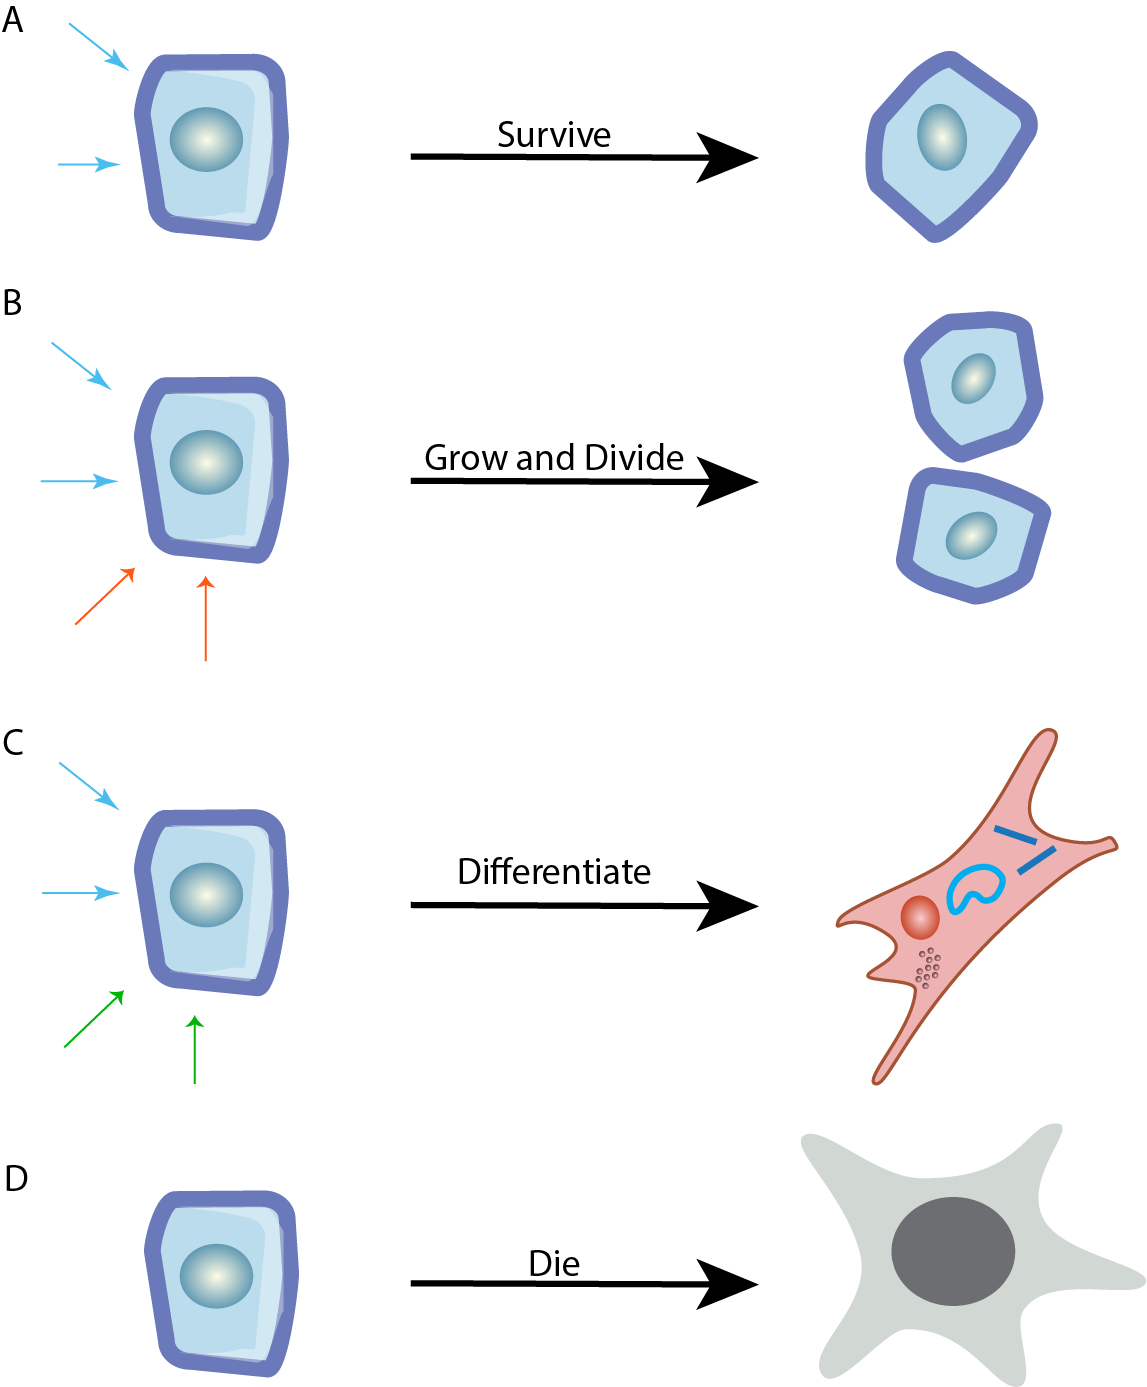
\includegraphics[width=0.6\columnwidth]{Chapter1/Figures/Chap1_figure1.png}
    \caption[Cell relies on multiple extracellular signalling molecules to survive.]{A cell can receive and respond to the signalling molecules produced by other cells using a set of receptors. The behaviours of a cell vary depending on the type of signals including to (A) survive (blue arrows), (B) grow and divide (red arrows) or (C) differentiate (green arrows). (D) The absence of survival signals can induce the cell suicide program known as apoptosis}
    \label{fig:Chap1_figure1}
\end{figure}

It is natural to make an analogy between the cell signalling systems and a human social organisation. This organisation relies on collaboration and coordination from multiple departments to operate successfully. The well-being of the individual is often compromised to benefit the whole. Similarly, cells in multicellular organisms heavily rely on interactions between individuals to be functional \cite{bartee2018principles}. Through advances in computational biology and experimental throughput, we can now intensively characterise these signalling mechanisms and even simulate the cell-cell signalling networks to better understand the principles of how interactions between cells can drive biological function \cite{sprinzak2010cis, teague2016synthetic, toda2019engineering}. Furthermore, technological development enables us to conduct more experiments in cells within living organisms \cite{helmchen2005deep, periasamy2013methods}, and spawns new means to study the cell microenvironment within a tissue context. 

Before discussing the approaches to studying cell-cell interaction in their spatial proximity, it is helpful to revisit the major types of communications that cells can perform. To perform communication, the cell secretes signalling molecules outside of the cell's membrane. The molecules can transmit across short or long distances and bind to receptors at the surface of the target cell's membrane. Some signalling molecules are so small and unstable that two cell membranes must be in physical contact to exchange signals. However, in most cases, signalling molecules can travel to distant cells in which the gradient of factor received can determine the behaviours.         

The interaction between cells, in which two cells are physically in contact, is called \textit{gap junctions}. These are specialized intercellular connections that link the cytoplasm of two adjacent cells via narrow-filled channels (Figure \ref{fig:Chap1_figure2}A). These channels allow cells to exchange various small molecules, and ions, but not macro-molecules, such as proteins or nucleic acids. The communication through gap junctions plays crucial roles in cell synchronization, differentiation, embryonic development, and immune response \cite{white1999genetic, vinken2006connexins}. For example, severe defects in heart development were found in mouse embryos to be caused by the mutation of one particular gap-junction protein (connexin 43) \cite{alberts2018molecular}.

While gap junctions are contact-dependent communications and allow cells to exchange ions or second messengers, cell communication also can take place across near or long distances. In most cases, signalling molecules are secreted outside of the membrane of signalling cells which act as local mediators to affect neighbouring cells in the immediate environment. Signalling that occurs over local distances local distance is called \textit{paracrine signalling}. In paracrine signalling, cells secrete signalling molecules called ligands and induce changes in nearby cells (Figure \ref{fig:Chap1_figure2}B). The ligand molecules in paracrine signalling tend to be rapidly absorbed by neighbouring target cells; destroyed by extracellular enzymes, or immobilized by the extracellular matrix. Prominent examples of paracrine signalling systems include neurotransmitters between nerve cells at a synapse,  blood clotting system, tissue repair, and formation of scars
\cite{huang1998gap}. 

Alternatively, the signalling molecules can also transmit through the circulation to act on target cells at far distant sites \cite{cooper2004cell, alberts2018molecular}. Distant signalling occurs when the molecules travel through the extracellular fluids to reach receiver cells called \textit{endocrine signalling}. Endocrine cells secrete their signalling molecules in the form of hormones, into the blood circulation, which sends the signal to targets cell throughout the body (Figure \ref{fig:Chap1_figure2}C). Signal transmission in endocrine systems is much slower than in paracrine signalling which in turn lasts longer as it relies on diffusion and blood flow. An example is pancreatic cells producing the hormone insulin which signals cells in fat, muscles, and liver to absorb glucose and maintain blood sugar levels.

\begin{figure}[htp]
% \renewcommand{\figurename}{Supplementary Figure}
    \centering
    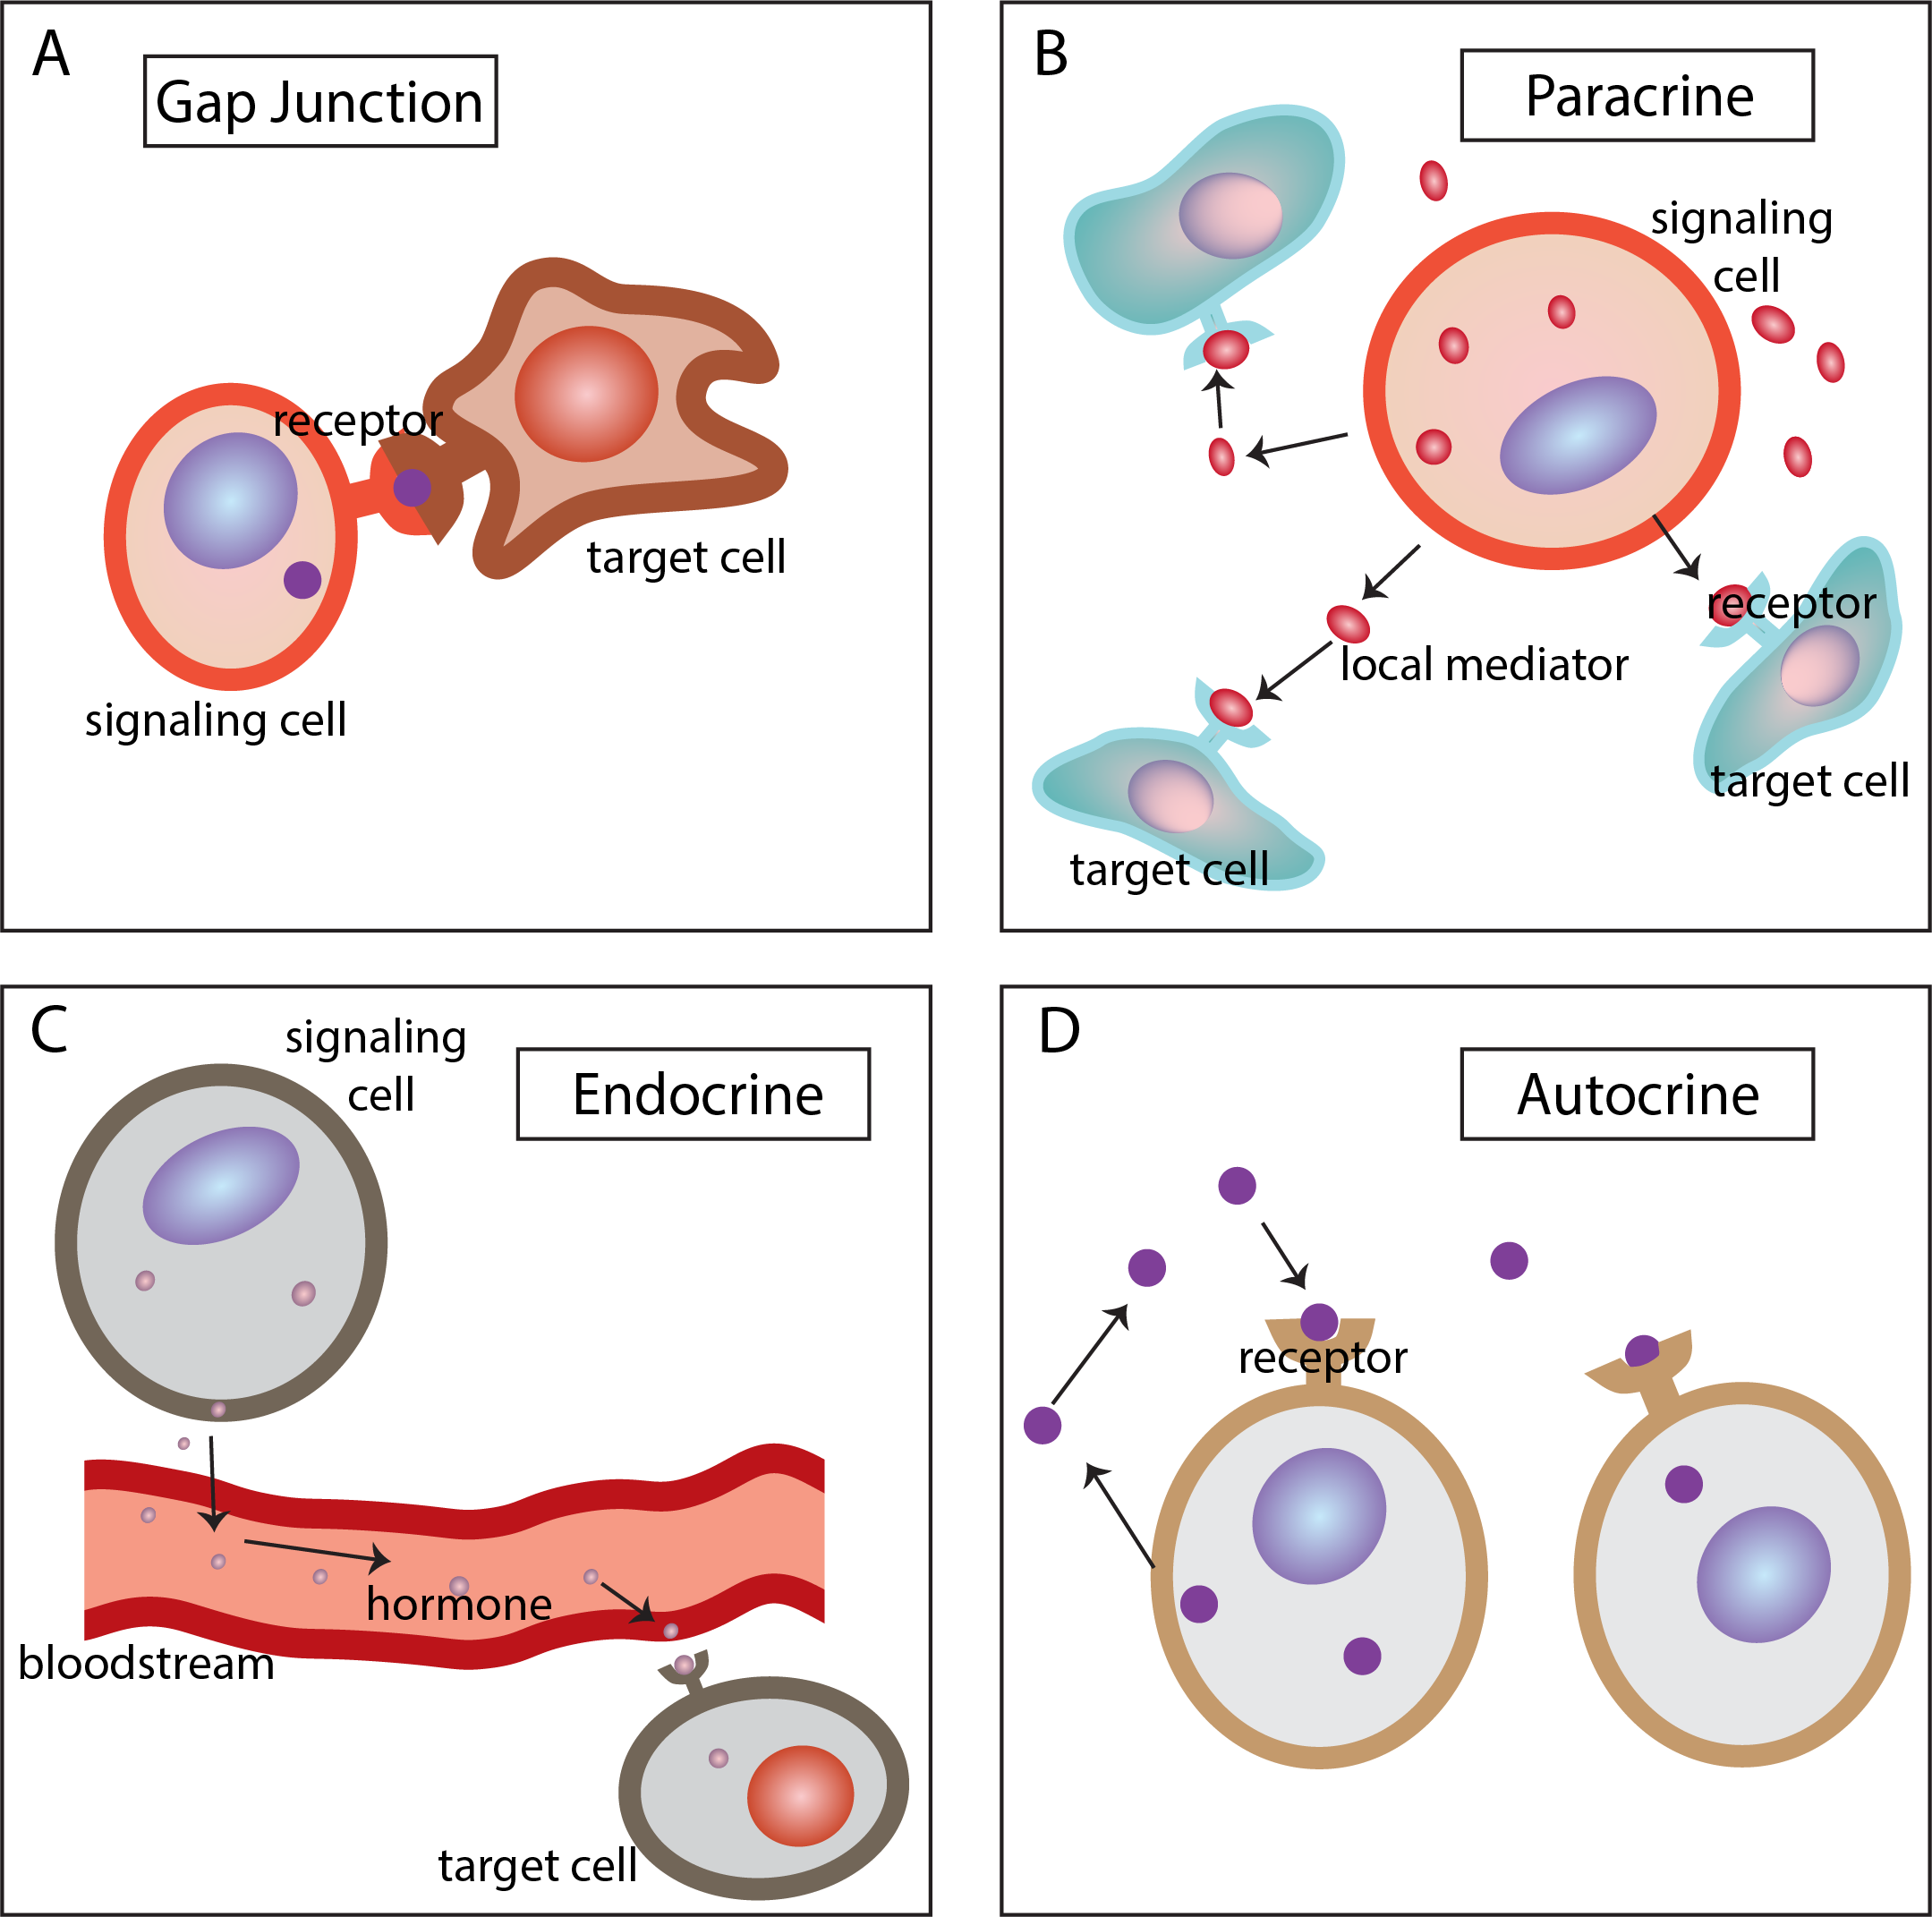
\includegraphics[width=0.8\columnwidth]{Chapter1/Figures/Chap1_figure2.png}
    \caption[4 Type of cell-cell interactions]{4 Type of cell-cell interactions: (A) Gap junctions is contact-dependent signalling which requires cells to be in the membrane–membrane contact. (B) Paracrine signalling does not require membrane-membrane contact, rather depending on local mediating signalling molecules that are released into the extracellular space and act on neighbouring cells. (C) Endocrine signalling depends on endocrine cells, which secrete hormones into the bloodstream for distribution throughout the body. (D) Autocrine signalling refers to cells secreting signalling molecules to induce the changes in the same cells}
    \label{fig:Chap1_figure2}
\end{figure}

In contrast, some cells can secrete signalling molecules to self-regulate or control other neighbouring cells of the same type. This type of communication is called \textit{autocrine signalling}. In \textit{autocrine signalling} (or intracrine signalling), cells stimulate themselves by sending the signalling molecules back to their own receptors. Autocrine signalling is most effective when occurring within the same cell or with neighbouring cells of the same type (Figure \ref{fig:Chap1_figure2}D). The process is used to encourage groups of cells to make the same developmental decision \cite{armingol2021deciphering, alberts2018molecular}. Thus, autocrine signalling is often found in cells that are differentiated along a particular pathway to reinforce developmental decisions \cite{alberts2018molecular}. Autocrine signalling is also often found in cancer cells and enhances cell differentiation and proliferation \cite{sporn1985autocrine}.  

Every kind of cell, from bacteria to complex, differentiated eukaryotic cells, can secrete chemical signals to perform cellular communication. The mechanism of cell signalling in single-cellular organisms such as yeast and bacteria has been well studied and understood \cite{alberts2018molecular}. Meanwhile, during the evolution of multicellular organisms, the signalling among cells achieved a high level of complexity. The crosstalks between different cell types from multiple tissues are crucial to every organism and form a complex microenvironment system to govern tissue functions. This is not only because the signalling methods are complex, but it is also because the number of cells present in the microenvironment can drive interaction to different outcomes. It is much more complicated to study the microenvironment system as a whole without a quantitative analysis and computational methods. Therefore, this thesis will hereinafter discuss only cell signalling in multicellular organisms, especially in humans. Toward the end of this chapter, computational approaches to investigate cellular communication in cancer will also be discussed to quantitatively uncover the complexity of the system. 

\subsection{The biological process of cancer}
In all multicellular organisms, each individual cell is a part of the whole cellular community and follows behaves in a socially responsible manner. To maintain the balance of the harmony of society, the number of cells in an adult body remains constant (around $10^{14}$ cells in an adult). However, throughout the lifespan, a cell can acquire some mutations which allow it to keep growing and dividing more than its neighbouring cells \cite{alberts2018molecular, greaves2012clonal}. Most of the mutated cells will be detected and either repaired or eliminated by the immune surveillance system in the body. However, cancer cells are said to be genetically unstable cells that accumulate enough mutations which give them \textbf{malignant} properties to break immunosurveillance and invade surrounding tissue. 

There are two malignant properties a cell needs to possess to be classified as a cancer cell. The cell needs to develop the mutations that allow it to (1) reproduce at an abnormal speed, and (2) be able to invade and colonize tissue sites normally reserved for other cells. An abnormal cell that either increase in size or proliferates out of control will give rise to a neoplasm \cite{alberts2018molecular, hanahan2000hallmarks}. The combination of the two properties contributes to the fatality of cancers. As long as the neoplastic cells have not yet become invasive, the tumour is considered as \textit{benign}. A tumour is considered as \textit{malignant} when its cells have developed the ability to invade neighbouring tissue. Metastability is a dangerous characteristic of cancer cells. It even allows cancer cells to migrate to another part of the body through the bloodstream or lymphatic vessels and form secondary tumours \cite{alberts2018molecular}. The further a cancer cell metastasises the more resistant to eradication it becomes.   

The abnormal reproduction of cells fosters tumour progression and tumorigenesis. Most normal cells in the body have built-in safety mechanisms which limit the number of successive cell growth-and-division cycles (Figure \ref{fig:Chap1_figure3}) \cite{hanahan2000hallmarks, hanahan2011hallmarksnext}. These safety mechanisms consist of two distinct barriers: \textit{senescence}, a typically irreversible entrance into a non-proliferative but viable state; and apoptosis, which involves cell death (Figure \ref{fig:Chap1_figure3}A). Cancer cells are found to contain mutations that can disable normal safety mechanisms which is either an increase in cell division or an inhibition of apoptosis. In addition to the capability to alter built-in cell senescence and/or cell apoptosis, cancer cells are also resistant to cell stress and DNA damage. The tumour grows because the cell birth rate outweighs the cell death rate, but often by only a small margin (Figure \ref{fig:Chap1_figure3}B-C). Therefore, the time that a tumour takes to double in size is only a gradual process.

\begin{figure}[htp]
% \renewcommand{\figurename}{Supplementary Figure}
    \centering
    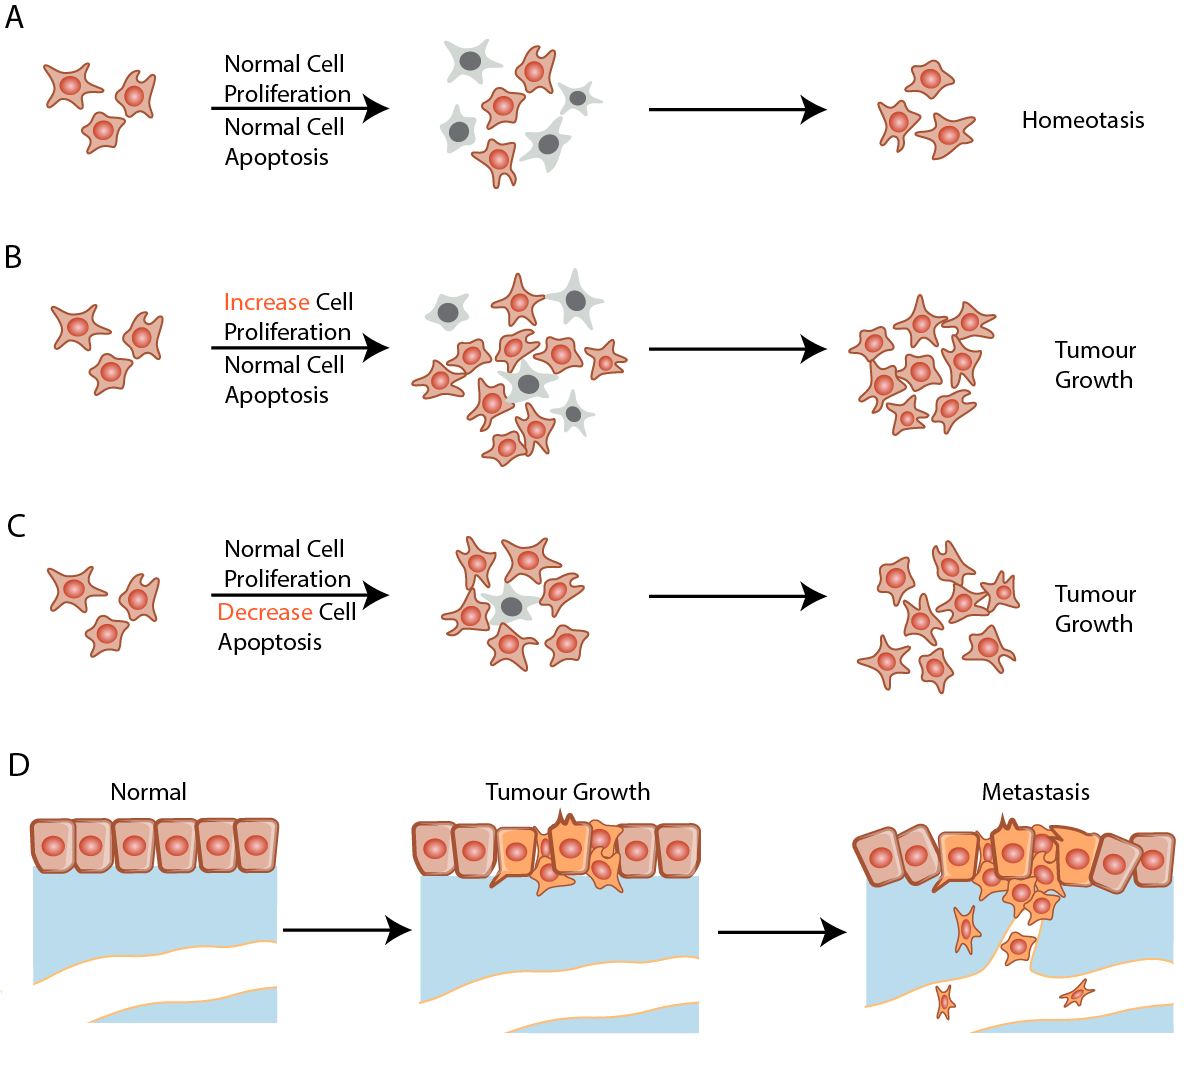
\includegraphics[width=0.7\columnwidth]{Chapter1/Figures/Chap1_figure3.png}
    \caption[Tumorigenesis and metastasis process. ]{The development of a tumour is the result of the mutated cells acquiring either stronger cell proliferation or inhibition of apoptosis (A-C). (D) An illustration of tumour cells resides from an organ to other organs through the bloodstream (figure adapted from \cite{alberts2018molecular})}
    \label{fig:Chap1_figure3}
\end{figure}

Metastasis is, in fact, a multiple-step process where cancer cells first invade locally, migrate to the circulation (lymphatics or bloodstream), and finally establish the new tumour at a distant organ. A cancer cell is dangerous due to its invasiveness and the ability to break free of constraints that keep normal cells in their designated organ \cite{greaves2012clonal}. Such properties are often acquired by the disorganized pattern of tumour growth and ragged borders, invading the neighbouring tissue. Fewer than one in a thousand malignant tumour cells that enter the bloodstream will colonise in a new organ and grow to the detectable secondary tumours \cite{joyce2009microenvironmental}. With modern blood test techniques, cancer cells can be detected early according to their surface properties while circulating in samples of blood from cancer patients. These biomarkers can inform the early treatment (\ie TP53, APC in colorectal cancer \cite{markowitz2009molecular}). Although cancer cells tend to avoid apoptosis, this does not mean that they are immortal. In the interior of a large solid tumour, cell death often occurs on a massive scale. However, cancer cells within the tumour often die from the necrosis process, which is unregulated death as the result of environmental perturbations. In necrosis, the cells become bloated and explode, releasing their contents into the local tissue microenvironment \cite{hanahan2011hallmarksnext}. Tumour necrosis factor (TNF$\alpha$) induces the upregulation of S100A8 and S100A9 in myeloid cells, which can also increase metastasis \cite{hiratsuka2008s100a8, hiratsuka2006tumour}. 

The dynamic of genetic mutations within cells is the major cause of tumour initiation. However, it is generally agreed that cancer metastasis is partially constrained by a complex, multifactorial interplay between cancer cells and the host tissue microenvironment. Some microenvironmental features can promote neoplastic cells including infiltrating macrophages and neovascularization. Mathematical modelling is an ideal approach to dissecting mechanisms of cancer invasion as it can simultaneously and quantitatively consider interactions between multiple factors \cite{anderson2006tumor}. The following sections will discuss deeper about a different type of interaction within cancer and aim to address the need for a computational approach.       

\subsection{The role of cell-cell interaction within cancer microenvironment}
Tumour growth and cancer invasion are landmark events with location-dependent \cite{friedl2011cancer}. It is often known that cancer originates from genetic instability. However, the growth of cancer cells into the tumour and the process of cancer metastasis are constrained by cellular interaction and tissue spatial conditions that dictate the interaction within and surround the cancer nest \cite{west2019cellular, liotta2001microenvironment,anderson2006tumor}. Cancer cells can produce growth factor ligands themselves, to which they can respond via the expression of cognate receptors resulting in autocrine proliferative stimulation. Many epithelium cells in breast cancer can produce its family of epidermal growth factor (EGF) ligands to stimulate cancer cells proliferation and motility, suggesting they may participate in autocrine and signalling with cells of the tumour microenvironment \cite{nickerson2013autocrine}.  

Cancer clone habitats are not closed systems \cite{greaves2012clonal}. A unique ability of cancer cells is their quick mutation to different environmental conditions, affecting cellular morphology in order to survive \cite{clark2015modes}. Tumours consist of not only cancer cells but also a whole microenvironment including endothelial cells, smooth muscle, fibroblasts and inflammatory white blood cells. Cancer cells in a tumour are the group of cells that have accumulated dangerous mutations; however, the development of a tumour indeed relies on two-way communication between the tumour cells and the surrounding environment (tumour stroma). In cancer pathology studies, the tumour microenvironment can influence cancer development in different ways. During early tumour development, the protection of the microenvironment surrounding the tumour fosters the tumour growth conditions such as chronic inflammation. As cancer progresses, the cancer cells secrete signal proteins such as TGF-$\beta$ and EGF to stimulate normal cells within the tumour to induce epithelial development as well as to modify the extracellular matrix \cite{beck2011systematic,BREMNES2011209}. The stroma, in turn, secretes signal proteins that stimulate cancer cells' growth and division (i.e. CXCL12) \cite{kumar2018analysis,wang2017role}. There is a feedback loop of cell-cell interaction between the cancer cell metastasis and the tissue microenvironments; in which the increase in intratumoral cell-cell interaction promotes collective migration in cancer \cite{friedl2011cancer, whiteside2008tumor}, leading to dynamically induced disorganization of nearby microenvironments of the tissue \cite{friedl2012classifying, canel2013cadherin, almendro2013cellular, roussos2011chemotaxis, zervantonakis2012three}. The prediction of tumour stroma and cancer cell crosstalks has created a therapeutic strategy that aims to block cancer cell interactions with the environments to create the growth-fostering habitat called "ecological therapy" \cite{pienta2008ecological, calabrese2007perivascular, bissell2011don}. Knowledge of heterogeneity within the tumour and stromal compartments remains essential to understand the cancer development and evaluation of treatment progress \cite{pages2010immune}.

In addition to the interaction between cancer and the stromal cells, crosstalk between cancer and immune cells is also closely connected to the tumourigenesis process including progression and metastasis \cite{wang2017role}. The role of the immune system is to protect the host from infectious pathogens and remove damaged cells \cite{davis2007molecular}. Macrophages have been determined to play roles in both tumour elimination and increase of tumour malignancy \cite{wyckoff2007direct, chung2005molecular}. In the early stage of cancer progression, immune cells such as macrophages and myeloid secrete paracrine signalling molecules (i.e. CFS-1 ligand)  to trigger a cell death process to eliminate cancer cells \cite{wyckoff2007direct}. If cancer cells are completely cleared during this elimination stage, immune cells will remain around the cancer cells to suppress tumour growth \cite{bronkhorst2011detection, ly2010aged}. Studies showed that the presence of tumour-infiltrating CD8+ T cells and Th1 cytokines surrounding the tumours associates with favourable prognosis in different tumour types including melanoma, breast, ovarian, and colorectal cancer \cite{fridman2012immune, shalapour2015immunity}. At a later cancer stage, metastasis happens when the cancer cells can mutate and acquire a phenotype that helps them to elude immune system surveillance. For example, the increase of PD-L1 expression in epithelial cancer cells causes CD8+ T cell exhaustion, which subsequently promotes metastasis \cite{chen2014metastasis, wei2019combination}. In other words, the continuous cross signalling between immune-cancer cells exerts selective pressure on the cancer cells to become more motile \cite{giampieri2009localized,ilina2009mechanisms}. The growth of the tumour can be categorised as the consequence of cross-cell type communication and morphological dependence. As a result, the modelling of immune-cancer cell interactions creates great opportunities for tumour management through the development of targeted therapy including immunotherapy. Understanding the signalling molecules that are used by tumour-associated immune cells in the different stages of cancer progression will provide insights into current development immunotherapies.  

% ***************************************************
\section{Experimental and computational methods for studying cell-cell interaction}
\label{section:lit_review}
The wide application of single-cell sequencing technology has successfully identified rare cellular properties, molecular features of cell populations, and cell-cell heterogeneity in cancer research. However, cancer tumours comprise multiple layers of signalling across cell types which are location-dependent, making them more heterogeneous than expected. Gene expressions in a cell are dictated not only by molecular profiles but also by space (i.e. its position in tissues and/or organs) and time (i.e. stage of cell cycle or developmental stage of the organ) \cite{salomon2020genomic}. Therefore, the ability to integrate single-cell molecular profiles with the spatial context in studying cell-cell communication can benefit research about the potential treatment of cancer.

In this section, I will review the current development of experimental techniques and computational approaches to study cell-cell interaction through spatial transcriptomics and proteomics. The advances in experimental technologies have quickly evolved in recent years (Figure \ref{fig:Chap1_figure5}). Together with new technologies to spatially profile transcripts and protein expression introduced in the past decade, numerous computational methods have been developed. While some analysis packages or pipelines were developed alongside the experimental platforms, most of the complex cell-cell interaction models were designed to be universal across experimental designs. The section \ref{Chap1:Sub_Spatial_Experiment_Platform} will thoroughly review the key technologies in spatial transcriptomic and spatial proteomic. In particular Visium, RNAscope, Nanostring CosMx for spatial transcriptomic and Polaris, Imaging Mass Cytometry for spatial proteomics. Next, I will review the studies of cell-cell interaction methods which consider either non-spatial or  spatial context in section \ref{Chap1:Sub_Computational}.                

\subsection{Experimental approaches to studying cell-cell interaction}
\label{Chap1:Sub_Spatial_Experiment_Platform}
In the past, intercellular communication was examined by measuring intercellular electrical signals in the cell membrane \cite{bennett1966physiology, loewenstein1967intercellular, de1982cell}. The presence of gap junctions allows cells to exchange a variety of ions and small molecules, thus they reflect the cell\'s electrical permeability properties \cite{penn1966ionic, bennett1966physiology,loewenstein1966permeability,loewenstein1974cellular}. By utilising such electrical properties of membrane junctions, cell-cell communication can be measured by injecting a cell with one of the microelectrodes and the adjacent cells (with presumed shared gap junction channels) with the other microelectrode. This method is readily applicable for tissue types with widespread cellular communication through gap junctions \cite{penn1966ionic}. It has been used to unveil differences between cancer and normal cells within liver tissues \cite{loewenstein1966intercellular, loewenstein1967intercellular}. However, the disadvantage of measuring electrical signals between cells is that they can be highly tissue-specific (i.e. liver, heart and lens tissues) \cite{gros1983comparative}. Additionally, the throughput of such an experiment is very low. Therefore, measuring cell surface electrical signals through gap junctions has become less popular in recent years. 

Recent advances in high-throughput microscopy, sequencing technologies and antibodies research have fuelled the development of two fields called \textit{spatially} transcriptomics and spatial proteomics. In fact, cell-cell interaction within tissue context is a multi-dimensional problem. The most intuitive way to capture cell-cell signalling is through the imaging approach. Either confocal or two-photon fluorescence microscopy can capture high-detail images of intracellular structures in a cell. While a specific review of these two types of microscopy is beyond the scope of this thesis, it is worth noting that they both use laser light to excite fluorophores, with the resulting fluorescence captured by detectors. A great feature of fluorescence imaging is the ability to monitor a number of specific probes simultaneously, thus allowing co-localization or multiparameter imaging of structures within cells or tissues \cite{periasamy2013methods}. There exist a number of fluorescently tagged protein biosensors, which can be used to track the movement of some ligand molecules in the studies of cellular and molecular interaction in healthy and diseased tissues \cite{gerdes2013cell}. Although a number of studies, in the early 2000s, have been done to model and quantify the activity of ligands and/or receptors \cite{awaji1998real, go1997quantitative, maamra1999studies, sneddon2003activation, bohme2009illuminating} using imaging data, they have limited scalability (Figure \ref{fig:Chap1_figure5}). The number of target ligands and/or receptors that can be measured per experiment is limited by the antibodies or RNA probes that can be used concurrently.    

Regarding spatial transcriptomics, it is a general term referring to capturing and quantifying gene expression of cells while retaining information of the tissue context \cite{burgess2019spatial}. There are several categories of spatial transcriptomic technologies. Current experimental technologies for spatial transcriptomics can be grouped into 4 major groups: (1) tissue microdissection-based approach, (2) RNA \textit{in situ} hybridisation-based (ISH) approach, (3) \textit{in situ} sequencing (ISS) approach, (4) \textit{in situ} capturing and \textit{ex situ} sequencing \cite{williams2022introduction}. Tissue microdissection-based is a brute-force approach to using a laser beam to dissect regions of interest from the tissue. These regions then undergo the RNA extraction and sequencing process. Due to multiple challenges in oncology settings and time-consuming, there are very limited spatial-omic studies utilising laser microdissection-based approaches \cite{wu2022spatial, wu2016spatially, junker2014genome}. Therefore, the following sections will discuss the other three spatially resolved transcriptomics approaches.

\subsubsection{\textit{In situ} hybridisation (ISH)-based}
\label{section:Imaging_sequecing_review}

An interesting analogy for detecting a specific DNA sequence on the chromosomes or in a cell is like looking for a needle in a haystack. The needle is the DNA sequence of interest and, the haystack represents all chromosomes. This search is made much easier if the investigator has a powerful "magnet"—in this case, a fluorescent copy of the DNA sequence of interest \cite{Connor2008natureEdu}. The first attempt to localize mRNA was conducted in 1969 and used radioactive labels and hybridization probes in the nuclei of frog eggs \cite{pardue1969molecular}. To this day, using radioactive probes is still available and is the most sensitive approach. However, the high cost of the experiment and potential hazards make radioactive approaches less favourable. Soon after the first experiment with radioisotopes, fluorescent labels made great strides in replacing radioactive probes because of their safety profile, stability, and ease of detection \cite{rudkin1977high, Connor2008natureEdu}. Since the first demonstration in 1994 (\cite{bassell1994single}), numerous RNA ISH methods based on the fluorescent ISH (FISH) approach have been developed, including single molecule FISH (smFISH), RNAscope, sequential FISH (seqFISH), multiplexed error-robust FISH (MERFISH), expansion-assisted iterative (EASI-FISH), and most recently DNA microscopy. 

Most of the currently developed technologies for RNA ISH are FISH-based and use fluorescently labelled probes that are hybridized to predefined RNA targets, to visualize the presence of transcripts. Probes are either directly or indirectly hybridized to the RNA molecules and subsequently visualized by microscopy. A benefit of RNA ISH is the ability to characterise the presence of RNA sequences within the tissue without cell dissociation. Although the basic principle of FISH remains unchanged, the sensitivity and multiplexing capabilities have advanced considerably. The first attempt to increase the sensitivity of FISH protocol was in 2012 with the release of smFISH (single molecule FISH) \cite{ji2012single}. By using a set of 5 short oligonucleotide probes (20-50 bp) to target multiple regions of a transcript, smFISH produces a higher and more robust signal. However, smFISH can only target a few genes at a time and inherits the limitation of spectral overlaps in standard microscopy technology.

There is an improved version of smFISH, called seqFISH, which allows capturing more transcripts at a time through serial rounds of hybridization, imaging and probe stripping \cite{asp2020spatially}. In seqFISH, the fluorescent probes are one-hot encoded and undergo a sequence of hybridisation. Each round of probe hybridization, imaging and probe stripping captures the presence of up to 24 different transcripts separately and enables the profiling of 10,000 genes \cite{moses2022museum,eng2019transcriptome}. However, an increased number of hybridization rounds is also associated with more expensive and time-consuming (approximately 10 hours to conduct one sequence of probe stripping). 

In an effort to side-step the extensive time of seqFISH, MERFISH was first developed in 2015 \cite{chen2015spatially} using probes with two flanking regions. After hybridizing to the RNAs, the fluorophores will bind to two flanking regions to facilitate the imaging process. For every round of RNA capturing, only fluorescent bits are removed while the encoding probes remain. Computational error-correction is performed after readout to account for imperfect signals in one round. Therefore, each round of hybridization in MERFISH is less time-consuming (around 20 min) than those in seqFISH \cite{moses2022museum}. Similar to seqFISH, MERFISH can also profile a maximum of 10,000 genes. Most of the FISH-based spatial technologies available use either seqFISH-based or MERFISH-based barcoding. 

While these methods have the advantage of multiplexed detection, the FISH technologies rely heavily on the fluorescent signal from the probes. To increase the sensitivity of FISH, signal amplification of either target nucleic sequences prior to ISH (e.g \textit{in situ} PCR) or signal detection after the hybridization process \cite{qian2003recent} can be used to enhance the quality of the image scanning. The signal amplification creates a quantification problem for RNA ISH and limits the application of RNA ISH in clinical analysis \cite{levsky2003fluorescence,wang2012rnascope}. Other RNA ISH technologies that can perform independent signal amplification such as RNAscope and DNA microscopy. While DNA microscopy is an optic-free mapping of nucleotides and does not rely on the physical location of cells, it is still a very new technology and has only been applied to a small subset of transcripts \cite{asp2020spatially,weinstein2019dna}. RNAscope technology is the more sensitive option for FISH which allows signal amplification and background suppression by itself.

Specifically, RNAscope assay is designed with ``Z-like" probes where the lower region of the Z is (18-25 bp) complementary to the target RNA and the upper region (14 bp) forms the binding site for the fluorescently labelled probes. Two assay probes with ZZ pairs are designed to bind in a region spanning 1000 bases of target RNA, this allows the specific detection and signal amplification from each target RNA molecule \cite{solanki2020visualization}. As a result, the RNAscope assay is best used for RNA sequences longer than 300 nucleotides. For short RNA sequences, a variant of RNAscope called BaseScope is a more suitable option. By using probe-specific amplifiers and sequence labelling, this assay can visualize multiple target RNAs simultaneously. Originally, RNAscope could only capture four different types of transcripts per experiment due to a limited number of spectrally discernible fluorescent dyes \cite{wang2012rnascope}. However, the latest version released in 2019, the Hiplex RNAscope assay has increased the number of RNA targets to twelve. Low multiplex RNAscope has been combined with another spatial proteomic technology called Imaging Mass Cytometry to capture both transcripts and protein simultaneously \cite{schulz2018simultaneous}. In comparison with seqFISH and MERFISH, RNAscope assays demonstrate lower multiplexing capability. 

To enable a faster imaging process while considering three-dimensional (3D) relationships of cells in thick tissue, expansion-assisted iterative fluorescence ISH (EASI-FISH) was introduced \cite{wang2021easi, borm2022scalable}. Before the ISH process, the RNAs within a tissue are preserved in a covalent attachment to the hydrogel mesh that covered the tissue. Next, the tissue in a gel is hybridized with several rounds of fluorescently labelled probes, followed by cytosolic DAPI staining and imaging under light sheet microscopy. The 3D image reconstruction is generated by registering multiple 2D images of DAPI images and the transcripts of fluorescent beads from different cycles via an affine transform. The transcripts in 3D space are assigned to a cell within a disc of radius from the nuclei. Recent commercial techniques for 3D FISH are developed under the Nanostring CosMx platform \cite{he2022high}.  

The probes used in the CoxMx platform consist of two components. The RNA target-binding domain of length 35-50 bp followed by 60-80 bp of a DNA readout domain (reporter-landing domain). The readout domain is separated into four sub-domains which can be hybridised with unique 10-20 bp reporter probes. Each reported probe can be encoded by four different fluorophores making 64 unique reporters that can be hybridised to the reporter-landing domain. Using that customisation, the CosMx platform inherits the capability to probe fluorescent signals in Z-stacked and alleviates the panel of RNA from 30 in EASI-FISH to 980-plex. Image registration is used to process 3D channel images from multiple rounds of hybridisation. An image processing algorithm is developed to detect the transcript fluorescent signal from the crowded reporter-binding event and assign it to the closest nuclei (within a radius of 0.5 pixels). Interestingly, the probe-encoded detection for RNA can be utilised for protein detection by replacing the readout sequences with antibodies \cite{he2022high}.   

The advancement of RNA ISH methods has not only allowed us to integrate the cells' functions with spatial information but also has expanded our understanding of the structural organization of normal and pathological tissues. FISH methods are becoming more popular in basic research. However, the use of that technologies in clinical routine is quite limited to validation of highly expressed genes (e.g EBER1/2 in EBV-related diseases) \cite{gulley2001molecular}. Over 10 tumour microenvironments  and 100 pairs of ligand-receptor specific for breast cancers have been discovered using the first demonstration of CosMx platform \cite{he2022high}. However, only a few methods have extended far beyond the inventor's laboratories and undergone successful commercialisation, including RNAscope, MERFISH, and CosMx \cite{conrad2022single}. 

\subsubsection{\textit{In situ} sequencing (ISS) technologies}
An alternative to FISH is adapting signal amplification and \textit{in situ} sequencing (ISS) of transcripts directly in the tissue. The concept of ISS methods is fairly similar to FISH when a panel of known sequence transcript is captured through the probes. The probes which have the padlock shape is a single-stranded DNA molecules containing the complementary sequence to the target transcript. Two ends of the padlock probes are closed by ligation, or by a DNA polymerase to create a rolling circle \cite{conrad2022single}. Sequencing by ligation is then used to read the actual RNA sequence of the transcript from padlock probes. The advantage of ISS approach over regular scRNA-sequencing techniques is the capability to link the sequencing back to the location of the probes. The number of genes that can be profiled by ISS is limited by the barcode length \cite{williams2022introduction, asp2020spatially}. Just like in seqFISH, only a small subset of all possible barcodes given a barcode length is used for error correction.

The first example of ISS approach for spatial transcriptomics was released in 2013 when it was used to profile the gene expression in breast cancer tissue. The padlock probe binds to the cDNA through hybridisation and produced the  clonally amplified rolling circle of the target cDNA sequences. The rolling-circle product is sequenced by ligation for RNA and sequence tag. Imaging for each round of probe ligation is carried out to capture the signal of the rolling-circle products located in the tissue sample. Similar to seqFISH, the sequential steps of probe ligation, imaging, and washing are iteratively carried out until the number of bases has been identified. Before being acquired by 10X Genomics, the original ISS platform can profile 31 targeted transcripts used in breast cancer prognostic expression panel \cite{ke2013situ}. The recent release of Xenium can now profile up to 400 genes concurrently. 

To achieve higher throughput of RNA transcripts, fluorescence \textit{in situ} sequencing (FISSEQ) combines the idea of fluorescently detection from FISH and cDNA amplification from ISS \cite{lee2015fluorescent}. First, a sequencing primer is hybridised into multiple copies of the RNA. Then, each RNA is \textit{in situ} amplified via rolling-circle amplification. The fluorescent probes are introduced to separate the difference between cDNA strands. After several rounds of hybridisation and imaging, the fluorescent tags are stripped off and the sequencing is performed. By using the sequential approach in seqFISH and MERFISH, FISSEQ has the potential to profile a few hundred to a thousand transcripts. However, FISSEQ has several disadvantages including low fluorescent sensitivity and a long imaging process.  

The ability to generate mRNA sequencing profiles with location is a powerful tool. With enough transcript detected, this approach could be used to characterise the tissue compartment in cancer tissue without prior information  \cite{ke2013situ}. Although ISS has the ability to detect SNVs that would be missed in FISH, the sensitivity of this approach was much lower compared to some regular FISH approaches. Besides, several problems regarding the sequencing process of ISS have been identified. While the sequencing dropout rate in regular scRNA-seq is $10\%$, most ISS approaches have a dropout rate over $70\%$. The loss of detection events may be due to many factors, such as the loss of the
mRNA from the tissue due to long fixation degradation and target sequence dependency. Both ISH and ISS suffer some similar technical limitations, in particular a requirement for many hours to days of imaging time on a microscope, thus generating terabytes of data. Finally, these methods require some trade-off between capture efficiency and the number of genes profiled. 

\subsubsection{Spatial barcoding and \textit{ex situ} sequencing}
Another concept is anticipated to be the more promising technology for spatial transcriptomics sequencing. The whole transcriptome of cells is captured and barcoded \textit{in situ}, followed by \textit{ex situ} sequencing \cite{asp2020spatially}. There are various experimental methods have implemented spatially resolved transcriptomics through this concept. Since the first one called Spatial Transcriptomic (ST) was established in 2016, there has been a series of new technologies introduced including Visum, GeoMx Digital Spatial Profiler (DSP) and SpaTial Enhanced REsolution Omics-Sequencing (STEREO-seq). 

RNA capture efficiency can greatly affect the quality of these methods, especially at higher resolution. Since most of the current existing technologies for \textit{ex situ} spatial transcriptomics sequencing (ST—seq) are new, they often require tissue-specific optimization. The standard capture resolution currently ranges from 2$\mu m$ — 100 $\mu m$ which means the capture rate is close to fewer than 40 cells. However, the experimental costs are considerably lower than for ISS. Due to the capability to profile the full transcriptome, this approach is gaining more popularity.          

Spatial transcriptomic by \textit{ex situ} sequencing (ST-seq) was among the first to be developed and later acquired by 10X Genomic in 2018. The first version of ST—seq published in 2016 used surface glass slides printed with barcoded probes grouped into circle spots. Each spot has a specific barcode id that is unique to the x and y coordinates on the glass slide. The tissue is fixed, imaged, and permeabilized on top of the spots. During the permeabilization process, mRNAs defuse out of the tissue and are captured by the probes. The final step is to reverse transcribe the mRNA and extract the barcoded cDNA-mRNA to sequence \cite{staahl2016visualization, berglund2018spatial}. The latest commercial kit of ST-seq is called Visium. Thanks to the advances in 3D printing, the diameter of barcoded spots are reduced from  100$\mu$m to 55 $\mu$m with a smaller distance between the spots.  Both  Visium  and ST-seq have already been used for the analysis of the tissue heterogeneity and gene expression in tumour tissues \cite{berglund2018spatial, thrane2018spatially, moncada2019integrating,ji2020multimodal, yoosuf2020identification} and inflammatory tissues \cite{carlberg2019exploring}. Results from the studies applied to cancer tissues again confirmed the role of the microenvironment in promoting tumour progression \cite{thrane2018spatially, moncada2019integrating}. Additionally, corresponding histopathology images of tissues stained with haematoxylin and eosin (H\&E) coupled with ST-seq allow the application of deep learning approaches for integrative analysis of histology images with the ST-seq profile \cite{he2020integrating, tan2019spacell}. Currently, protocols to enable recovery of mRNA from FFPE tissue sections for legacy ST-seq or Visium are being extensively developed to facilitate higher sequencing depth.           

Besides Visium, STEREO-seq from BGI is another ST-seq platform that features \textit{in situ} capturing of whole transcripts and performs \textit{ex situ} sequencing. STEREO-seq captures the RNAs using an array of nanoballs printed on the chip. The standard nanoball in the chips has a size of approximately 2.2 $\mu$m diameter which is substantially smaller than the diameter of the capture spots in the Visium array. While tissue permeabilisation and RNA sequencing also follow the same principle of the other ST-seq approach, STEREO-seq outperforms Visum and legacy ST-seq or Visium with the ability to measure tissues at subcellular resolution.    

Given the complexity and heterogeneity of tumours, untargeted methods like Visium and STEREO-seq can extend the capacity to study immune cell infiltration both in localized and metastatic diseases. In comparison to RNA ISH or ISS, ST-seq provides sub-optimal spatial resolution. However, with the advantage of the whole transcriptome profile, ST—seq is undoubtedly a promising complementary technology to FISH and/or ISS.  
% \subsubsection{Barcoded-targeted sequencing and }
% \subsubsection{Spatially barcoded probes and ex situ sequencing}
% These techniques are generally transcriptome wide, but do not have single cell resolution; the resolution is the size and shape of the spots and spacing between the spots. In ST and Visium, the array is constructed by printing the capture sequences onto commercial microarray slides, so the 5’ end of the sequences are attached to the slide; where each spatial barcode is placed is known. 

\subsubsection{Fluorescent-based spatial proteomic technologies}
Similar to spatially resolved transcriptomics, spatial proteomics often refers to the set of methods that use imaging technology to capture the presence of proteins in their native cellular environment without the need for the physical separation of cells or organelles before proteomic analysis. In addition to understanding the morphological context of RNAs, the spatial distribution of proteins is also equally important in studying cancer. Protein localization directly connects to protein function in health and disease. Being able to capture the localization of proteins and their dynamics at the cellular level is essential for a complete understanding of cell biology \cite{lundberg2019spatial}. 

There are several technologies to visualise the presence of proteins within the spatial context. These approaches are often grouped on either highly multiplexed imaging or mass cytometry imaging technologies. Similar to FISH technologies, multiplexed imaging is a fluorescence-based/colour-based approach and involves iterative rounds of staining, imaging, and removal of signals. Immunofluorescence (IF) and immunohistochemistry (IHC) are technologies used for visualizing cellular components, especially proteins which are categorised into the multiplexed imaging approach. They were invented in the 1904s by Albert Coons \cite{coons1941immunological} and remain a cornerstone in pathology and health care. Since the development of IHC and IF, the number of studies that used these techniques has grown exponentially. These methods are commonly applied by the cellular biology, biochemistry, pathology and immunology fields and reflect the particular value of IHC and IF in researching diseases.        

IHC is a general term for the techniques that use antibodies or enzymes to identify specific proteins (antigen markers) in cells within tissue sections. The antibodies are specific and are expected to only bind to the targeted proteins. There are many different ways to perform visualization of targets in tissues with IHC or IHC-based methods. However, based on the experimental settings, IHC can be categorized into two groups: colourimetric and fluorescent. In colourimetric IHC, the antibodies or enzymes bind to proteins and trigger coloured precipitation which becomes visible to standard light microscopy \cite{BOURGEOIS2014132}. The enzymatic reaction or coloured precipitation keeps producing products as long as there is no more regent or physical space to deposit more reactant \cite{corthell2014basic}. Consequently, the colourimetric staining IHC is permanent in the tissue section and can be used for qualitative analyses where quantification is not considered important \cite{seidal2001interpretation}. 

Visualization of antigens by fluorophore-conjugated antibodies is also often referred to as IF \cite{joshi2017immunofluorescence}. Unlike colourimetric IHC, fluorescence IF is not stable over long times and can only be observed after excitation with specific wavelengths \cite{corthell2014basic}. The antibody, when excited emits light of a different wavelength. IF also inspired the use of fluorophore-conjugated probes to directly visualize specific DNA and RNA sequences in the tissue which is often referred to as fluorescent \textit{in situ} hybridization (FISH). There are two different fluorescence assays available for detecting antigens which are categorized by whether a single antibody or two antibodies are used, namely direct and indirect IF \cite{JOSHI2017135}. The former protocol is simpler and used for labelling abundant target proteins with a primary protein carrying a fluorophore that binds to a specific antigen. Meanwhile, the indirect IF protocol requires multiple stages of incubation; a primary antibody that binds only to the target and a secondary antibody with fluorophores to attach to the primary antibody. The primary antibody in indirect IF can allow multiple secondary antibodies to bind to it, creating signal amplification effects. Therefore, indirect IF is a better choice for detecting low-abundance targets. In comparison to colourimetric IHC, the benefit of using fluorophores is that they label multiple targeted proteins in the same tissue sample. However, unlike colourimetric staining, fluorescent labelling is not permanent. Since the fluorescent signal generally reflects the concentration of bound antibody \cite{dabbs2017diagnostic} IF is considered a better choice for a quantitative experiment.

Due to relatively low costs, IHC and IF have been playing a central role in the visualization and identification of tissue antigens as well as in clinical diagnosis and prognosis for years \cite{ducheyne2015comprehensive, rupprecht2015current}. Depending on the purpose of the experiments and tissue preservation technique, IHC or IF be used interchangeably. While IHC studies are routinely used for pathological clinical diagnosis, the IF technique is the method of choice when an experiment requires investigation of colocalization of multiple proteins \cite{joshi2017immunofluorescence}. IHC and IF can be done on fresh frozen tissue yet most IHC is performed with Formalin-Fixed Paraffin-Embedded (FFPE) tissue. An example of the application of immunostaining in a clinical context is the use of IHC to evaluate the presence of HER2 in breast cancer sections. By using IHC and antibodies to detect HER2 receptors, clinicians can diagnose the current status of the patient to better decide on treatment options. Clinically, immunostaining is used for histopathology for the diagnosis of specific types of cancers based on known molecular markers.  

% [Polaris]
The results of IHC and IF heavily rely on the antibodies of choice and the capabilities of the technician performing them. Many studies highlighted that the choice of the antibody panel and the interpretation of the reaction patterns are the most important factors for  clinical outcome \cite{de2010immunohistochemistry, jensen1997immunohistochemistry}. In laboratory science, immunostaining by IHC and IF is limited by the number of protein markers it can feature at one time. Thus, IHC and IF are still being optimised for better performance in a multiplexed manner \cite{joshi2017immunofluorescence}. It is worth noting that protein visualization using fluorescence-based staining remains a good option. Polaris, as an example, provides a multiplex IHC based on the OPAL technology that can capture up to 9 proteins with very high quality. High-throughput multispectral scanning from Polaris can produce a whole slide scan of 6 biomarkers in 6 minutes ($1x1.5cm$ tissue section) \cite{hoyt2021multiplex, baharlou2019mass,marc201934th}. The increase in signal accuracy can reduce the false colocalisation and signal crosstalk between biomarkers. The average signal intensity for all the markers has been validated to be within the recommended range ($10-30$) \cite{donovan2021924}. With a specific design, multiplexed IHC-based experiments can facilitate the study of cell-cell interaction through spatial proteomic technology.  
% []

Additionally, there are multiple technologies for multiplexing fluorescence-based protein staining including GeoMx Digital Spatial Profiler (DSP) and co-detection by indexing (CODEX). In GeoMx DSP, a multiplexed cocktail of primary antibodies with  unique ultraviolet-photocleavable DNA oligos is used to target the proteins. After exposure to ultraviolet light from the GeoMX instrument, pools of released indexing oligos were hybridized to the optical barcodes and then read by another instrument (e.g NanoString nCounter or Illumina MiSeq) \cite{de2020unraveling, helmink2020b}. This enables to simultaneous detect up to 96 proteins and over 900 RNA targets. The disadvantage of GeoMx DSP is that the platform only captures average transcripts level within predefined regions. The disadvantage limits the use of GeoMx DSP in investigating cell-cell interaction as the predefined regions may vary in shape and cell count. 

On the other hand, CODEX has been developed by the inventor of MIBI and also uses a specialized instrument to convert images from fluorescence microscopes into highly-multiplexed imaging systems. CODEX currently allows the detection of over 60 protein markers within the tissue by iteratively staining and scanning the tissue sections\cite{goltsev2018deep}. Similar to OPAL Polaris and other traditional multiplexed IF platforms, CODEX enables the capture of protein expression at the single-cell level. If the protein panel is specifically designed, CODEX can facilitate the analysis of cell-cell interaction analysis. High-level landscapes of cell types pairwise interaction in mouse spleen and human colorectal cancer have been investigated using the CODEX dataset \cite{schurch2020coordinated, goltsev2018CODEX}. A disadvantage of CODEX, but also of many other FISH-based technologies and IMC, is the lack of signal amplification which results in the under-detection of lowly abundant protein/gene markers. A comparative overview of three different approaches to performing spatial proteomic is shown in Table \ref{table:SpatialProteomicComparison}. 

\subsubsection{Mass Cytometry Imaging Technologies}
In addition to more recent advances in IHC and IF, there is another branch of development in the spatial proteomic platforms that capture protein expression using mass spectrometry. Recent developments in flow cytometry, high-throughput microscopy and mass spectrometer have allowed us to apply conventional protein study strategies in a spatially resolved context. The first wave of spatial proteomics methods used mass cytometric (MC) analysis. As an off-shoot from IHC/IF technology, MC-based spatial proteomic methods use mass-tagged antibodies to visualize the protein. An advantage of this type of analysis approach is that it can easily be used to study proteins in many different cell types. Two notable technologies have been developed that are based on the MC approach including Hyperion Imaging Mass Cytometry (IMC) as the pioneer and Multiplex Ion Beam Imaging (MIBI) as the direct competitor platform. Both methods use antibodies conjugated to stable metal isotopes. In IMC, after the tissue section is immobilized on slides, the tissue is stained with panels of antibodies then it enters a laser ablation chamber where it is rasterized until it plumes. The aerosolized/ionized plumes of tissue are fed into a time-of-flight mass spectrometer to analyse isotope abundance.  There was a study that combined two technology of RNAscope and IMC workflow to interrogate the interplay between transcription and protein in the tissues \cite{schulz2018simultaneous}. Instead of fluorophores, the RNAscope probes are modified to tag with metal. Thus mRNA and protein can be simultaneously measured in single cells. By using pure and rare-earth element isotopes, IMC can overcome the limitations of spectral overlap observed in IF and allow quantifying up to 38 tagged channels simultaneously. However, the use of lasers damages the tissues that are being scanned. A study of breast cancer using IMC as a sole experiment has identified multiple features of the tumour microenvironment and cell-type colocalisation that are associated with clinical outcomes \cite{jackson2020single}.

Alternatively, MIBI can be used to image histological sections labelled with isotope-tagged antibodies. Most of the steps for measuring protein levels using MIBI are similar to IMC \cite{baharlou2019mass}. However, in MIBI secondary ion mass spectrometry is needed and  an (oxygen) ion beam is used instead of laser ablation to raster over the tissue. Subsequently, ions are analysed using a mass spectrometer. While the MIBI only ablates a thin layer of the tissue (20-50nm) and causes less damage to the tissue section, the technology creates signal interference effects and makes quantification more challenging \cite{bodenmiller2016multiplexed}.

Besides, there is another technology called Mass Spectrometry Imaging (MSI) that characterises protein expression using a mass spectrometer. Matrix‐Assisted Laser Desorption/Ionization (MALDI) tissue imaging is a technology using this approach and has been proven to be more versatile than MC. In MALDI, a laser and mass spectrometer are used to ablate the tissue and ionize the molecules. Eventually, the ionized molecules are fed to the spectrometer to determine the molecular weights \cite{caprioli1997molecular}.  This is performed in a label-free manner to measure the proteins present in the tissue. In this way, MALDI is more suitable for non-targeted experiments. However, there are also a number of limitations for MALDI or MSI in general such as lower spatial resolution, reduced sensitivity for larger proteins, and low multiplexing capability. 

The quality of multiplexed mass spectrometry imaging and staining technologies is anticipated to gradually approach the current level of standard IHC and IF in the research lab \cite{bodenmiller2016multiplexed}. However, until the new technologies are fully matured, clinicians would still rely heavily on the use of IHC and IF  \cite{de2020unraveling}.
\begin{table}[ht]
\centering
\caption{Feature comparison of spatial proteomic technologies}
\begin{tabular}{||P{3cm} || P{3.5cm} || P{2cm} || P{2cm} || P{2cm} ||} 
 \hline
   & Staining IF   & \multicolumn{3}{c||}{Mass tagged antibodies} \\  [0.33ex] 
 \hline\hline
 Technologies & CycIF, CODEX, NanoString DSP  & IMC & MIBI & MALDI   \\ 
 \hline
 Resolution & $\sim$600$\mu$m-single cell  &  $\sim$1000$\mu$m & $\sim$260$\mu$m & 50-200$\mu$m \\
  \hline
 Repeat analysis  & Yes  &  No & Yes & Yes \\
  \hline
Maximum epitopes  & $\sim$60-96 & $\sim$40 & 40 & $<$10   \\ [1ex] 
 \hline
\end{tabular}
\label{table:SpatialProteomicComparison}
\end{table}
\subsubsection{Challenges and general considerations}
Studying cancer as a system is complicated by the heterogeneity caused by the intratumoral diversity, and variations across lesion sites and patients. By using single-cell data of dissociated cells, we can gain insight into cell type identification within a cancer tumour (Figure \ref{fig:multimodal_approach_cci}A-B). At the molecular level, studies have used scRNA-seq to investigate the microenvironment of several cancer types including prostate cancer \cite{miyamoto2015rna}, breast cancer \cite{brady2017combating}, melanoma \cite{tirosh2016dissecting} and colorectal cancer \cite{li2017reference}. However, these studies were limited to identifying the population of cancerous cells and did not further investigate crosstalk between cell types in the cancer microenvironment. Besides the loss of tissue morphology due to cell dissociation, we reason that until recent years, we did not have the technologies necessary to retrieve highly-throughput information from a tissue \cite{bodenmiller2016multiplexed}. Therefore, the combination of multiple spatial omics is preferred to resolve the complexity of cell communication in cancer (Fig.\ref{fig:multimodal_approach_cci}) \cite{de2020unraveling}.   

Although spatial transcriptomic and proteomic experiments provide a comprehensive, spatially resolved view of cell types and the locations of cells in tissues, modelling the network of cell-cell interaction demands computational methods. The amount of data from multiplexed spatial-omics data poses several computational challenges in preprocessing the data and constructing computational pipelines \cite{wu2022spatial}. Firstly, we need reproducible standards and computational platforms that can perform analysis on multiple or all highly multiplexed imaging data types \cite{bodenmiller2016multiplexed, schuffler2015automatic}. Secondly, the choice of cell segmentation hinders the development of modelling cell-cell interactions in the spatial context. To study cellular interactions at the molecular level, we need to demarcate individual cells from the tissue image. This process requires image segmentation to identify the cell's coordinates and boundaries. Thirdly, while there are several batch-correct algorithms designed for scRNA-seq that are still suitable for spatial transcriptomic data analysis (i.e. Seurat \cite{butler2018integrating}), data normalisation still remains a challenge in spatial transcriptomics and proteomics data analysis. For translational research, a large cohort of patient samples with associated clinical information is often used. The computational models of cellular interaction should be able to include clinical and genomic features to account for the high-order relationships between interaction and clinical outcome. The following Sections \ref{Chap1:Sub_Computational} will review the computational progress of spatial-omics analysis and how these methods boost multi-modal spatial data analysis.  

\begin{figure}[hbt]
    \centering
    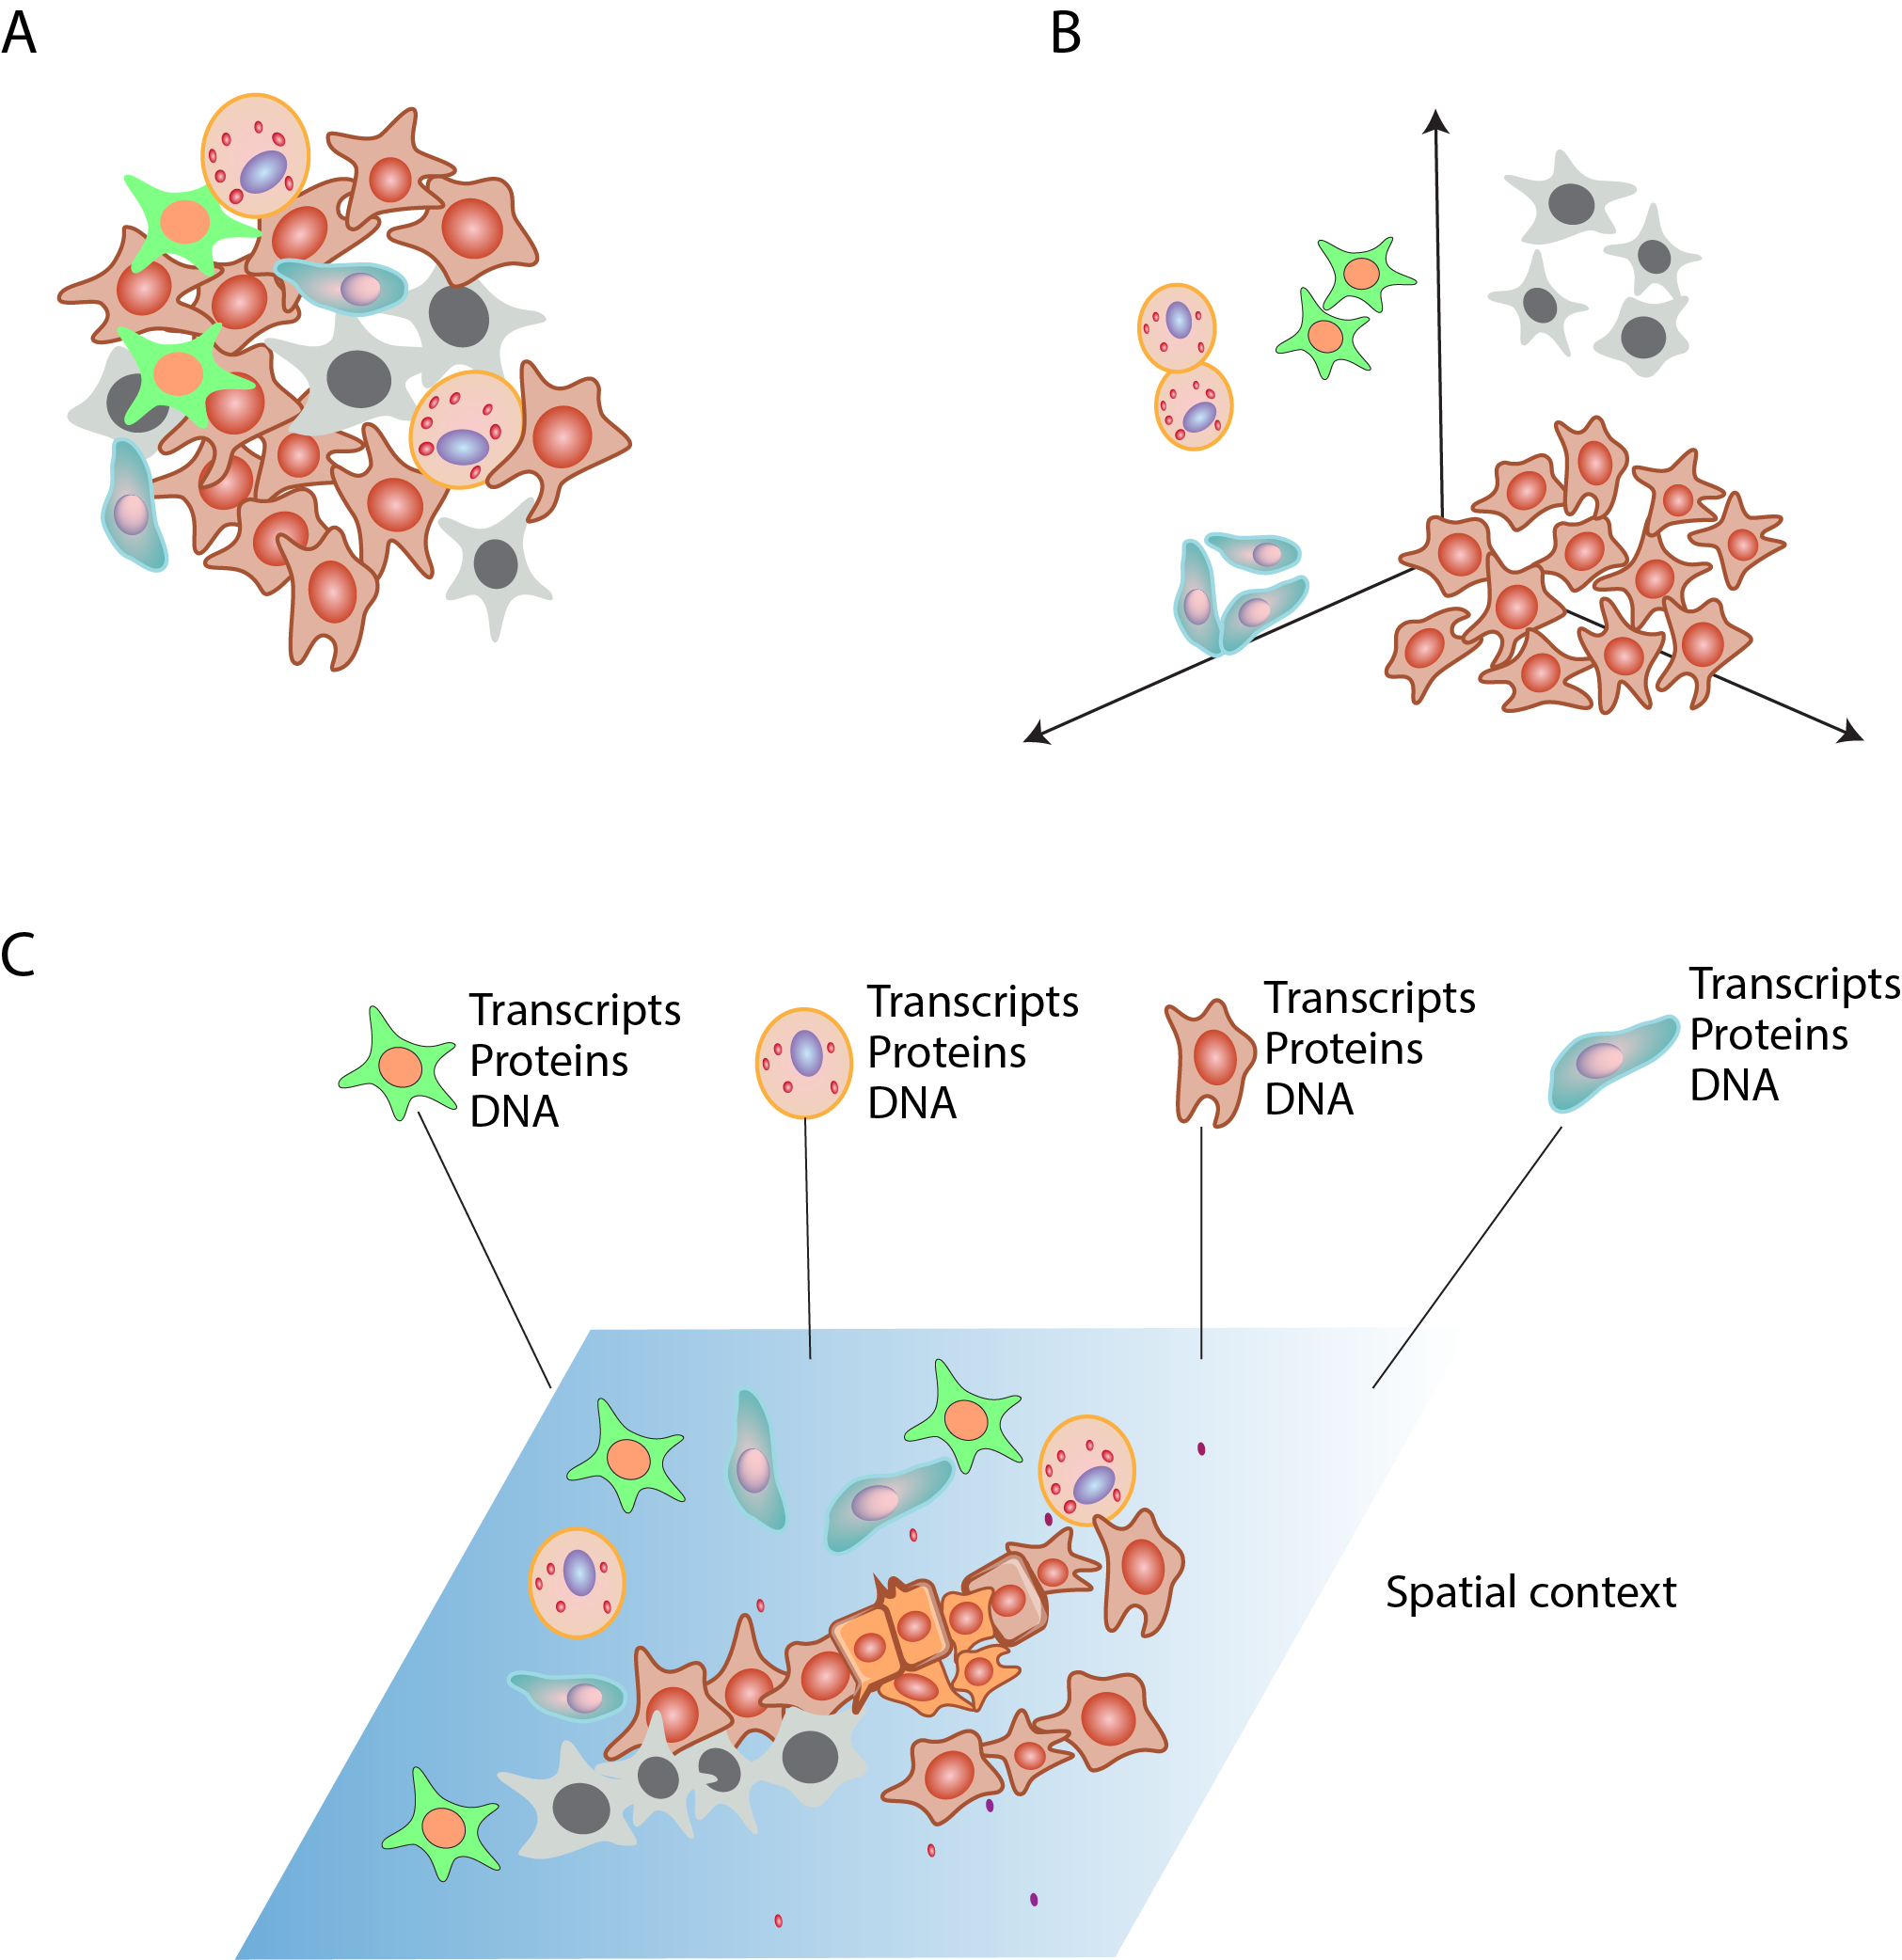
\includegraphics[width=0.7\columnwidth]{Chapter1/Figures/Chap1_Figure5.png}
    \caption{Approaches to studying cell interactions in cancer (A) Intratumoral heterogeneity of the cells within a tumour microenvironment. (B) Three-dimensional projection (e.g. UMAP of scRNA-seq data) of individual cells after dissociation. (C) Measure each cell via multi-omics data including proteome, transcriptome, and genome within the spatial location. (Inspired figure from \cite{de2020unraveling})}
    \label{fig:multimodal_approach_cci}
\end{figure}

% \subsubsection{}
% \subsubsection{}
\subsection{Computational methods to study cell-cell interaction within spatial context}
\label{Chap1:Sub_Computational} 

As discussed above, an important feature of the cellular phenotype is its morphology. While scRNA-seq data can provide information about gene expression in cells, cell morphology is about cell physical features such as locations, area, perimeter, solidity, eccentricity and circularity. Additionally, both gene/protein expression and cell morphology are important features, especially in a disease context. The emergence of multiplexed spatial analysis enables dissecting the tumour microenvironment at multiple levels and higher granularity. 

\subsubsection{Cell-cell interaction inference using scRNA-seq based data}
To perform the computational study of cell-cell interaction, we need to address the two disadvantages of (1) a limited number of markers and (2) a lack of information on spatial location. The widespread use of single-cell data, over the past few years, in the form of single-cell RNA sequencing (scRNA-seq) has unveiled rare cellular functions and biologically meaningful cell-to-cell variability. Many computational methods have been proposed to infer the ligand-target links between cells from scRNA-seq data such as CellPhoneDB \cite{efremova2020cellphonedb}, NicheNet \cite{browaeys2020nichenet}, SingleCellSignalR \cite{cabello2020singlecellsignalr}, NATMI \cite{hou2020predicting} and iTalk \cite{wang2019italk}. While scRNA-seq loses the spatial information, the method can measure a higher throughput of transcripts. Cell dissociation is required in order to perform the scRNA-seq experiment. The dissociation procedure causes a loss of cell coordination information, making it challenging to link the transcriptomes back to their original spatial location. As discussed, the spatial context in cancer is a critical component for studying cell-cell interaction. Subsequently, these packages for cell-cell interaction inference from scRNA-seq data are used as biomarker discovery tools and required validation \cite{de2020unraveling}. 

To overcome the lack of spatial information from scRNA-seq prediction, a complementary approach that integrated multiple modalities with scRNA-seq data and spatially-resolved data has been used. Integrating spatial context into studying cell communication would greatly improve the justification of the ligand-receptor inference result and satisfy the grasp for modelling intratumor heterogeneity and cell communication during tumour development \cite{crosetto2015spatially, pages2010immune, marusyk2012intra,bedard2013tumour}. Recent studies combined scRNA-seq to spatial transcriptomic to locate the interaction within immunosuppressive tumour-specific keratinocyte subpopulations in non-melanoma skin cancer \cite{ji2020multimodal}. Such integrated data may offer insight into clinical prognosis. However, there is still a gap in computation when integrating spatial proteomics with scRNA-seq data. In many cases, a third experiment is required for a holistic integration \cite{ji2020multimodal, schulz2018simultaneous, govek2021single}.    

\subsubsection{Ligand-receptor interaction inference using spatially resolved -omic data}
Given the advances in spatial-omic experimental methods, we can now capture simultaneously up to 900 different transcripts and 40 protein markers from a sample. It is natural to ask whether we can perform cell-cell interaction from spatial-omics data independent from scRNA-seq data \cite{moses2022museum}. Current ST-seq platforms have not yet been able to provide as deep sequencing as scRNA-seq platforms do; however, they can, to some extend, shed light on the niches enriched for certain gene sets \cite{Bost2022Optimizing}. Many of the genes are encoded for either ligands or receptors which cells use to signal others. Expression of L-R pair of the cells in close proximity is often used to identify cell-cell interaction. To trace the spatial cellular communication dynamics, several computational approaches have been developed to model cell-cell crosstalk from spatial-omic data. Various methods are developed for for inferring cell-cell interactions based on known L-R pairs from spatially resolved -omic data, including stLearn, Giotto, SpaOTsc or GCNG \cite{pham2020stlearn, dries2021giotto, cang2020inferring, yuan2020gcng}.  

stLearn \cite{pham2020stlearn} uses the curated CellPhoneDB database \cite{efremova2020cellphonedb} as the reference to make predictions about the L-R pairs that co-express by the cells from ST-seq data. The p-value of significant coexpression L-R is computed by the permutation test of the observing L-R pair against the null distribution. The regions or spots with diverse cell types and high p-value of L-R coexpression in neighbouring spots are identified as regions where cells are likely to signal each other. 

squidpy \cite{palla2022squidpy} is another package that uses CellPhoneDB and infers cell-cell interaction through L-R pair. squidpy re-implemented CellPhoneDB at the backend to utilise the list of L-R existing from the input data. Given a pair of query cell types, squidpy permutes the cell types in the cell-cell neighbourhood network to build the null distribution of the expression of each L-R pair. For each permutation, the mean expression of the two molecules for the L-R grouped by query cell types is calculated. A P-value for significant pairs of L-R is computed by comparing the permuted means against the ground truth mean.

A similar strategy is used in Giotto \cite{dries2021giotto} which identifies cell-type colocalisation by an unsupervised correlation-based analysis. Giotto constructs a network representation of the pairwise interacting cell types and labels the edges of the spatial neighbourhood graph as homo- or heterotypic. From the cell network, for each L-R pair from a known database, a co-expression score is assigned for all cells that have the heterotypic edge. p-value and log2 fold change of the spatial permutations were calculated to test whether the cell types are more or less likely to colocalize than expected from completely random cell type localization. Within one cell type (cells that have the homotypic edges), Giotto uses classical DE (Student’s t-test, Wilcoxon rank sum test, limma, and permutation of spatial locations) to find DE genes between neighbours of cells of another cell type and non-neighbours.

In GCNG \cite{yuan2020gcng}, a slightly different neighbourhood network is constructed using the K nearest neighbours approach. By default, the neighbourhood graph connects a cell to 3 nearest neighbours. GCNG performs cell-cell communication analysis using the location of the cells and the expression of gene pairs (gene expression level ligand and receptor) in each of these cells. Then both the gene count matrix and the normalized Laplacian of the neighbourhood graph are fed into a graph convolutional neural network (GCN). The GCN can then predict novel pairs of genes involved in L-R signalling, and if trained on the direction of interaction in the L-R pairs. While stlearn, squidpy or Giotto can perform the cell-cell interaction through the L-R pair on both ST-seq and multiplexed FISH data, GCNG can only work with multiplexed FISH data. 

\subsubsection{Cell types colocalisation analysis}
The spatial structure of the tissue is a heterogeneous collection of single cells, consisting of various multiple homogeneous and heterogenous groups \cite{schurch2020coordinated}. There are also methods that identify such regions independent of identifying spatially variable genes and/or gene patterns \cite{moses2022museum}. In this approach, the computational approaches focus on identifying spatial colocalisation throughout the tissue using cell type information (Fig: \ref{fig:CCC_conceptualised}A). 

For each cell across the tissue, the spatial identity of itself is defined by a $K$ number of nearest neighbouring cells (including itself as the reference). The nearest neighbour metric is measured by the Euclidean distance between the $X$ and $Y$ coordinates of the cells in the two-dimensional tissue section. Alternatively, we can also apply a neighbourhood identification method that is threshold-free, known as the Delaunay cell network \cite{guibas1985primitives, dries2021giotto}. The spatial identities of cells are then clustered by their neighbourhood features \ref{fig:CCC_conceptualised}. The clusters of cells based on cell neighbourhood (i.e. spatial identity) can reveal communities of cells within the tissue and the composition of cell types for each community. Such methods have been used and adopted in different fields including eco-geography as well as biology \cite{goltsev2018CODEX, dries2021giotto}.

Several spatial analysis packages consider each cell as a point in a 2-dimensional coordinate system. The advantage of this point-process approach is that it can use most of the analytical procedures established in high-level spatial analyses in social studies \cite{yushimito2012voronoi}. In squidpy, cells are considered as points representing cell centre coordinates \cite{palla2022squidpy}. The spatial neighbourhood network of cells is also constructed using cells as nodes and neighbourhood relations between spots as edges. There is a variety of options to build the relationship network including $K$ nearest neighbours, radius distance or Delaunay triangulation. Several computational packages apply this strategy to construct the spatial network of cells for downstream interaction analysis such as spicyR, Giotto or ATHENA \cite{canete2022spicyr, dries2021giotto, martinelli2022athena}.    


Histocat's neighbourhood analysis uses statistical methods to find significantly enriched interactions between or within a cell type. 
\begin{figure}
    \centering
    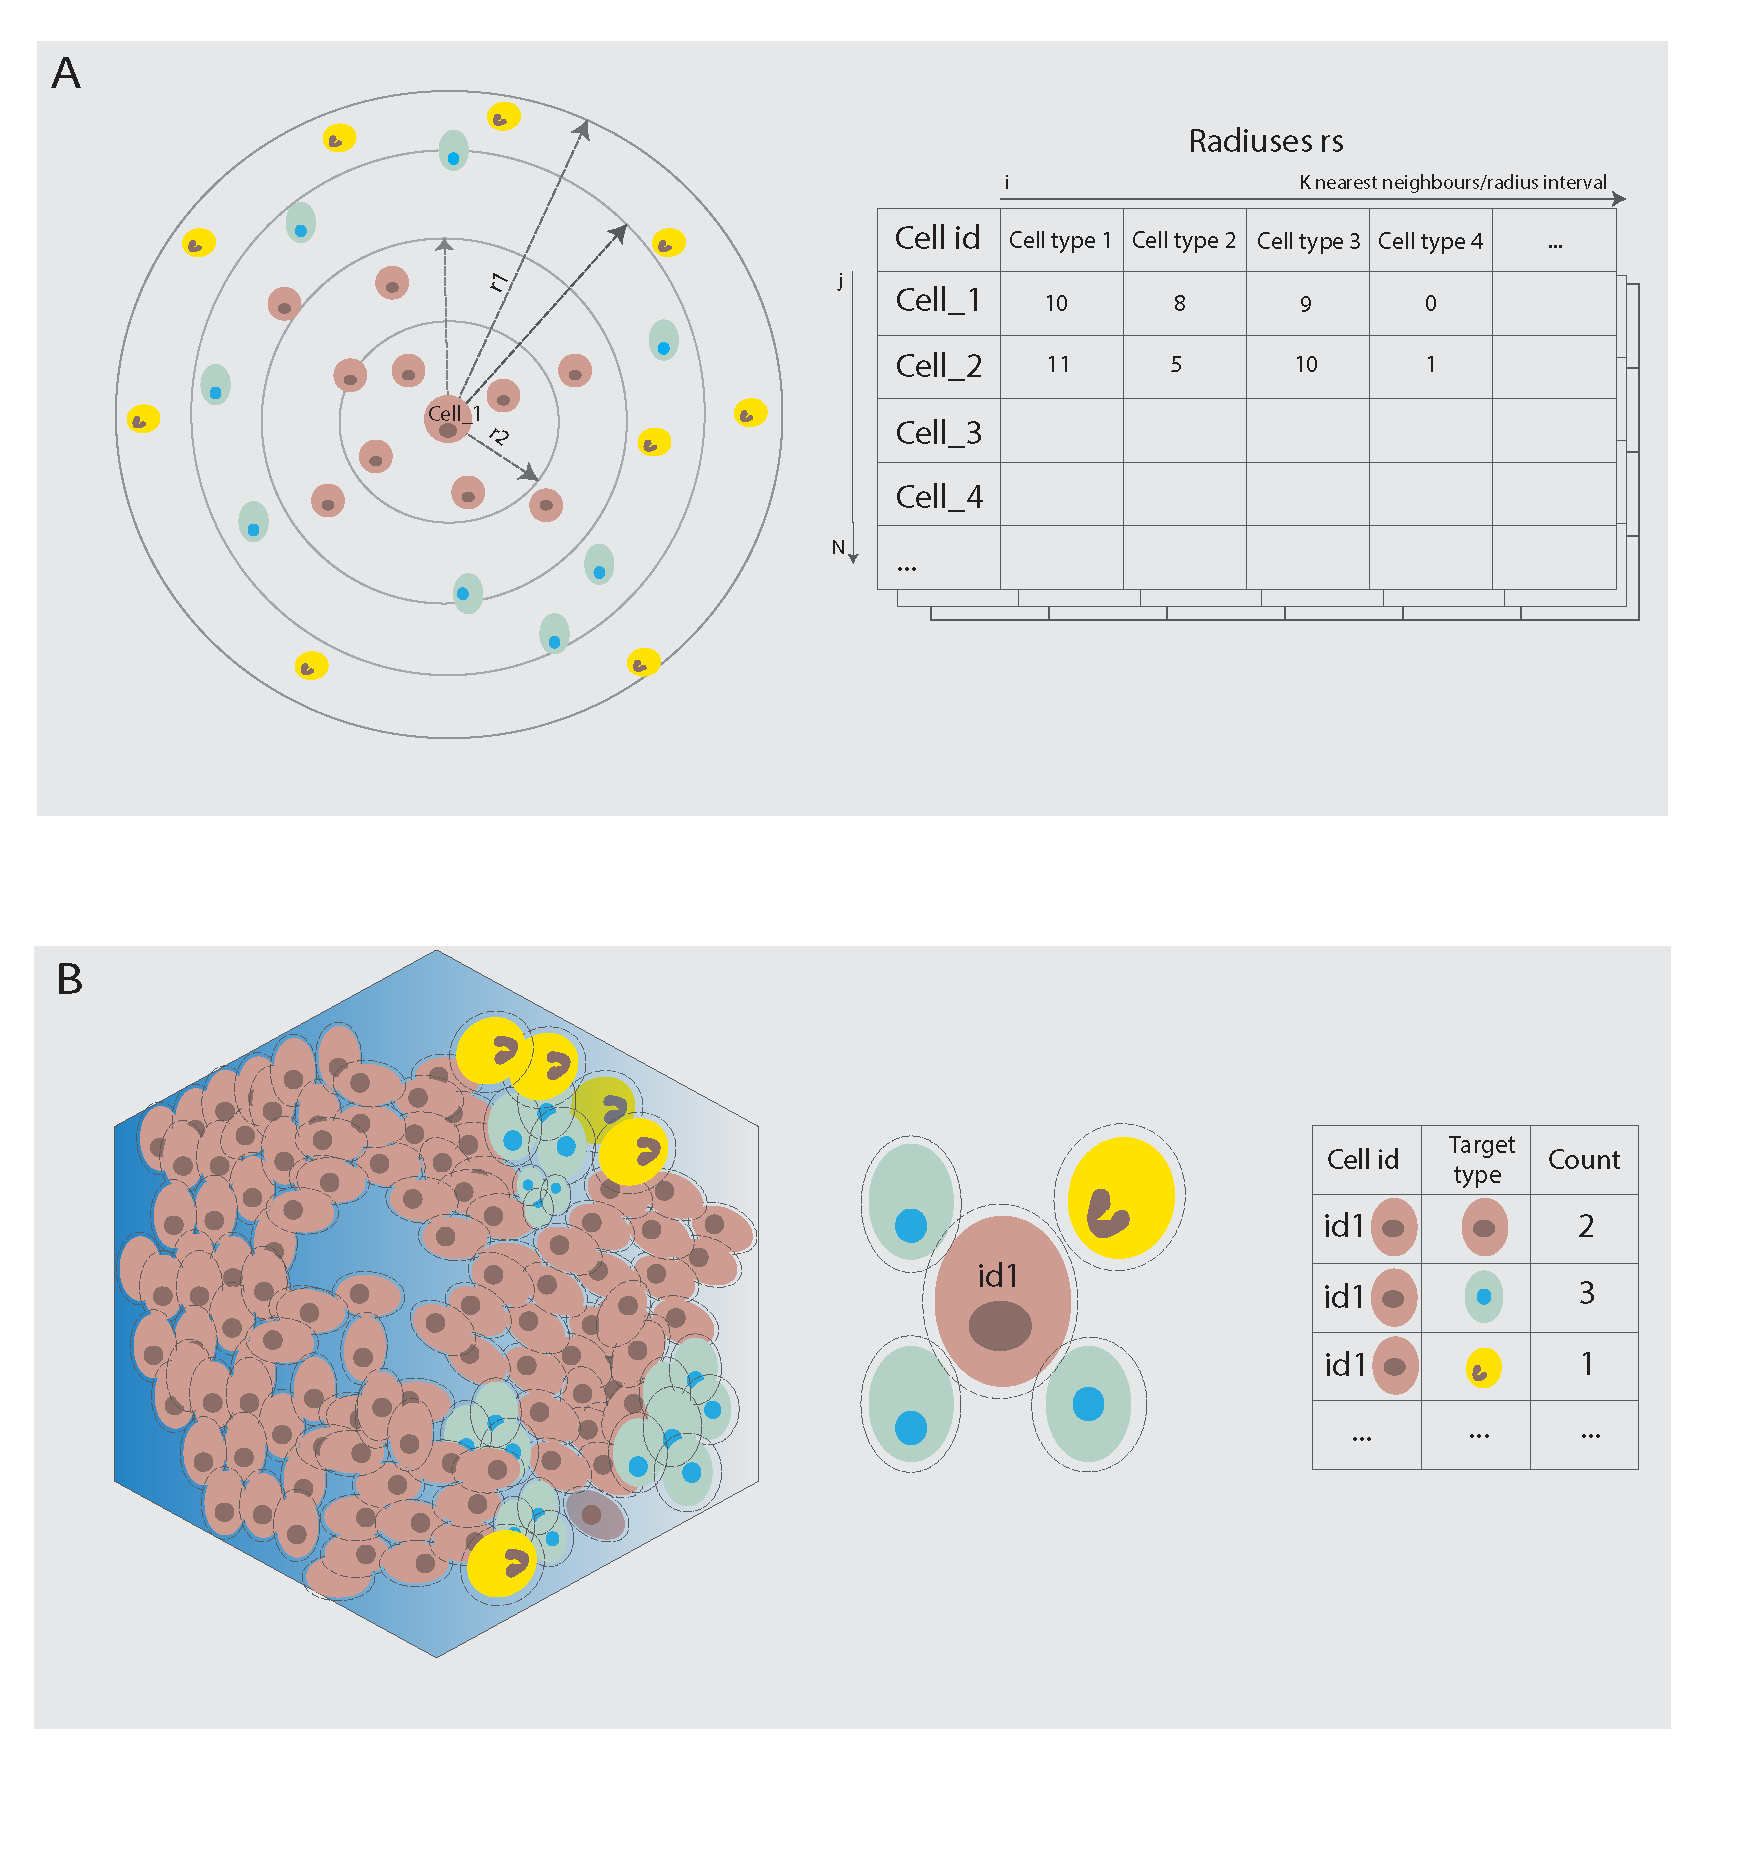
\includegraphics[width=0.85\columnwidth]{Chapter3/Figures/Conceptualise_CCC_analysis_cropped-01.png}
    \caption[Summary of different cell type interaction analyses.]{Summary of different cell type interaction analyses. (A) Schematic of cell-cell interaction through varying distance intervals. The analysis process starts by iterating through every cell and then aggregating the information about neighbouring cells to determine the cell spatial identity. (B) Schematic of measuring spatial interaction of cells through counting the number of touching cells. Randomising is applied downstream of the analysis to identify the significance of pairwise interaction}
    \label{fig:CCC_conceptualised}
\end{figure}

% Spatial variance component analysis (SVCA) (Arnol et al. 2019) models the expression of each gene of interest among the cells as a 0 mean Gaussian process. The covariance h
% [...]
Despite the described experimental advances in imaging and sequencing technologies, there are limited computational approaches that have been developed to enable and expand the analysis of spatial data. Most open-source tools that provide image-linked data analysis workflows were typically developed for low-plex fluorescence microscopy (e.g IHC and IF) and were not geared to applications in analysing highly multiplexed measurements. Some emerging open-source software tools provide highly interactive graphic interfaces and are more user-friendly such as QuPath, CellProfiler and HistoCat \cite{bankhead2017qupath, carpenter2006cellprofiler, schapiro2017histocat}. These open-source software programs have the advantage of customising analysis modules which allow users to implement and optimise the analysis scripts for their own data and questions. It is also worth noting that open-source software programs are widely popular among the research community. Thus, community support and troubleshooting discussions for the usage of these open-source software are more available  than those of commercial software. 

Meanwhile, there is a number of analysis packages that do not provide a graphical interface but can control functions inside such as Spatial Seurat and scanpy. The advantage of having control of analysis through script is that they allow addressing specific questions and users may be able to modify the scripts for scaling up the analysis for larger data or sample sizes. These packages are more suitable for bioinformaticians and those who have a computational background. However, packages like Seurat and scanpy often do not use spatial information, with a much more focus on scRNA-seq profiles. It is necessary to interrelate and utilise layers of information obtained from spatially resolved omic data. There is an essential lack of analysis software that can properly address the need to incorporate multiple types of data as well as provide the capability to scale up the analysis.


\label{subsec:ST_seq}

\section{Research Objectives}
The rise of immunotherapy is substantially changing the cancer treatment paradigm \cite{dobosz2019intriguing}. However, often less than $30\%$ patients respond to a single treatment type \cite{ott2017combination}. In addition, immunotherapy is also associated with a variety of severe autoimmune-like side effects \cite{naidoo2015toxicities,bertrand2015immune}. These can be attributed to heterogeneity among single cells within the tissue. Technologically, single-cell multimodal omics integration is recognized as the method of the year for 2020 by Nature Methods \cite{teichmann2020method}. By simultaneously measuring multiple modalities, it is expected that different aspects of one cell can be revealed at a time. Thus, multimodal spatial data can greatly inform the discovery of relationships among cell types by exploring shared patterns across -omics data types \cite{teichmann2020method}. The expansion of spatial-omics data further improves our understanding of different angles of cellular communication in cancer, contributing to finding rational immunotherapy agents. Both discovery and translational research goals in a study on cellular communication rely on the integration of spatial-omics datasets. This thesis will be focused on adapting and developing analysis methods to combine spatial omics data, in the forms of imaging and sequencing data, to investigate intercellular communication.   


% The overarching hypothesis of thesis is: \textbf{a large number of cell-cell interactions in cancer can be identified and characterised by spatial omic data.}. 
\section{Thesis Overview}
\subsection{Developing a spatial transcriptomic analysis method named STRISH to study interaction via colocalisation analysis in SCC/BCC skin cancer samples}

Chapter 2: Using Spatial Transcriptomic and single-cell RNA sequencing for cell-cell communication. 

Cell-to-cell communication underscores a dynamic cellular ecosystem that develops, evolves, and responds to environmental factors. The implications and roles of cell-to-cell communication have been investigated extensively, particularly in cancer, using a wide range of in vitro and in vivo techniques, albeit at different scales and resolutions \cite{brucher2014cell}. Breakthroughs arising from discoveries in cell communication have led to important clinical applications. 
% A classic example is the interaction via immune checkpoint proteins \cite{pardoll2012blockade}. Tumor cells, tumor infiltrating lymphocytes and tumor associated myeloid cells express inhibitory PD-L1/CTLA4 ligands to engage PD-1 receptors on cytotoxic T cells and CD80/86 receptors on myeloid cells, effectively blocking immune activation against the tumor cells. The discovery has led to applications of using monoclonal antibodies that specifically target this ligand-receptor (L-R) interaction as a form of immunotherapy, allowing immune cells to suppress cancer growth \cite{weiner2012antibody}. Therapies targeting these two pairs of ligand-receptors have transformed the management of several cancers, including melanoma, renal cell carcinoma, bladder cancer, head and neck cancer, and many others \cite{ott2017combination}. Notably, often less than 20\% of patients respond to a single immunotherapy, including common cancer types like breast, colon and prostate cancer \cite{ott2017combination}, and hence the urgent need to combine therapies, for example by using antibodies against PD-L1, CTLA-4 and/or PD-1 \cite{ott2017combination}. However, mechanisms of action for combinational immunotherapies remain elusive \cite{wei2019combination} and the number of current druggable targets for cancer-immune cell interaction is extremely limited, compared to the large repertoire of over 2,000 known ligands and receptors. Therefore, research to explore and advance understanding of known and new ligand-receptor pairs in the context of tumor-immune cell interaction within a tumor is extremely important for the further development of immunotherapies \cite{weiner2012antibody, helmy2013cancer}. 

Chapter 2 derives from the idea to utilise the ST-seq data to study cell-cell interaction throughout the skin tissues. I developed a computational analysis pipeline called STRISH to detect all possible cell-cell interactions through ligand-receptor across neighbouring spots in ST-seq data. To validate the finding from ST-seq, I used the highly sensitive FISH with RNAscope to capture the presence of two ligand-receptor pairs of markers that have been identified as involved in paracrine signalling in skin cancer. Additional to RNAscope validation, digital droplet PCR was used to quantitatively measure the molecules from tissues for comparison with RNAscope results. Extending from measuring RNA, I applied the STRISH method to detect protein, covering the whole tissue and at subcellular resolution. Opal multiplex IHC can measure 4-7 proteins on the same tissue. While the experimental frameworks are accessible, all the scRNA-seq, ST-seq, RNAscope and IHC data require computational analyses to quantitatively process the sequencing and imaging data so that cell-cell interactions can be inferred from and compared across datatypes. Lastly, the computational methods were applied to locate the cell-cell interaction through PD1 and PD-L1 using Polaris spatial proteomic as the second validation with target-specific technologies. The overall structure of chapter 2 will be presented in two parts as below:     
\begin{enumerate}[align=left]
    \item[\textbf{2.1}] Use ST-seq data to study cancer-immune cell communication.
    \item[\textbf{2.2}] Validate the findings from ST-seq using other target-specific technologies.
\end{enumerate}

\subsection{Overview of the analysis results in skin and colorectal cancer using spatial proteomic data}
We reasoned that the interactions between cell types within the tissue are beyond the cellular level, happening at a higher-order scale. Cells within the tissue are organised into multiple compartments and structures with distinct functions. By analogy, different cell types in the spatial context are considered individuals with different roles and functions (i.e. teachers or doctors) in human society. At a higher granular level, the tissue communities are equivalent to facilities that are specialised in functions. Therefore, identifying the interaction at the different granularity and integrating information between them allows us to better understand the tissue's behaviour \cite{schurch2020coordinated}. Advances in experimental technologies and computational methods have allowed the association analysis between the tissue spatial communities and clinical outcome or genomic alteration \cite{schurch2020coordinated, danenberg2022breast}. For this chapter \ref{Chap:3}, I focused on the high order of spatial organisation and the cross-talk between cell types in cancer tissues.

Chapter 3 will focus on using the spatial proteomic data to study the cellular organisation within the cancer tissue as complementary to the spatial transcriptomic from chapter 2. While the number of gene markers that can be profiled using cutting-edge spatial transcriptomic is growing rapidly, e.g. Visium (10X Genomic) \cite{thrane2018spatially, moncada2019integrating,ji2020multimodal},  Stereo-Seq (BGI) \cite{wei2022single,chen2022spatiotemporal}, it is important to note that not all RNA expression is highly correlated with translated protein expression level. Besides, spatial proteomics is also an important tool to uncover the complex heterogeneity of cancerous cells and their intercellular connection with other cells \cite{arnol2019modeling, jackson2020single, bodenmiller2016multiplexed}. Advances in multiplexed tissue imaging enable the analysis of up to a hundred proteins in thousands of cells in a single experiment. The protein profile of tissue has been analysed; it can provide an additional layer of connection from cells to environmental context and biological processes. 

Chapter 3 will address the following topics:    
\begin{enumerate}[align=left]
    \item[\textbf{3.1}] Use spatial proteome profiling data to inform the cell type composition in the tissues.
    \item[\textbf{3.2}] Correlate cell types and interaction within their spatial context to understand the physiological state of the tumour microenvironment.
    % \item[\textbf{3.3}] Quantitative and qualitative measurements of cell neighbourhood network
\end{enumerate}

Two types of spatial proteomics data are analysed. Polaris as multiplexing IHC for nonmelanoma skin cancer samples, a panel of 6 biomarkers was used to profile the protein expression of every single cell within a tissue section. For the second dataset, a spatial proteomic profile, using the IMC platform, of 126 ROIs from 52 patients with stage 3 colorectal cancer is studied. The advantage of using the IMC platform is that it allows capturing the protein expression of using rare-earth isotopes not present in a biological system and therefore more specific. 

% \begin{table}[ht]
% \centering
% \caption{Summary of data specification}
% \begin{tabular}{||P{7cm} || P{3cm} || P{3cm} ||} 
%  \hline
%  Specifications & Colorectal Cancer Samples & Skin Cancer Samples   \\ [0.33ex] 
%  \hline\hline
%  Number of patients & 52 & 3   \\ 
%  \hline
%  Number of Markers & 16 markers & 6 markers  \\ 
%  \hline
%  Number of images & 126 ROIs &  6 whole slides \\
%  \hline
%  Diagnosis & Stage 3 adenocarcinoma & Basal Cell Carcinoma  \\ [1ex] 
%  \hline
% \end{tabular}
% \label{table:DataInfor}
% \end{table}

As described in section \ref{section:lit_review}, multimodal omic measurement offers a holistic view of cells in their native context. Spatial proteomics can be a complementary method that can provide confirming or new information compared to the cellular transcriptomes. However, the availability of analysis workflows and methods for spatial proteomics and integration with transcriptomics is still limited. The aim for chapter 3 will focus on adapting the spatial analysis methods of spatial proteomic data to shed light on cell types and communities defined at the protein level. From identifying different cell compartments that reflect cancer heterogeneity, the spatial colocalisation of these cells also suggests the cellular interaction across the tissue microenvironment.             

\subsection{Overview of chapter 4: MOSAP multiple omics spatial analysis platform}
As Chapter 2 and Chapter 3 use spatial-omic data to study cell interaction with a focus on individual tissue analysis, chapter 4 aims to elevate from applying the methods developed in Aims 1 and 2 to multiple patient samples. The ultimate goal is to visually understand cell interactions, especially immune-cancer cell interactions. I will demonstrate the power of MOSAP integrative analysis methods and workflows on two specific cancer types including skin cancer and colorectal cancer.

Chapter 4: The association between tumour spatial structures and clinical diagnostics or subtype classification
% \begin{enumerate}[align=left]
%     \item[\textbf{4.1}] The variation of tumor microenvironment structures in skin cancer
%     \item[\textbf{4.2}] The tumor microenvironment analysis across patients in colorectal cancer samples
%     % \item[\textbf{Aim 4.}] Quantitative and qualitative measurements
% \end{enumerate}


\subsection{Overview of chapter 5: Conclusion}

Spatial omics is an emerging but rapidly developing topic. This thesis has contributed to the early development of analysis methods in the context of cellular communications in cancer. In the concluding chapter, I will discuss the pros and cons of the methods developed here, and provide future perspectives on applications and interesting further research directions. 
Chapter 5: Discussion and future plan
\begin{enumerate}[align=left]
    \item[\textbf{5.1}] Applications of analysis methods to study multiplexed imaging data, potentials, strengths and limitations. 
    \item[\textbf{5.2}] Future perspective
\end{enumerate}


% \bibliographystyle{elsarticle-num}
% \typeout{}
% \bibliography{./References/Bibliography}
% \printbibliography[heading=subbibliography]

%CHAPTER 2
%If you are presenting work which has been previously published, acknowledge this here.
% ***************************************************
% How to introduce a previously published chapter
% ***************************************************
%This is an example of how you might introduce a chapter that has been published previously. 
\cleartoevenpage
\pagestyle{empty}	

% ***************************************************
% Example of an internal chapter
% ***************************************************
%This is an internal chapter of the thesis.
%If you have a long title, you can supply an abbreviated version to print in the Table of Contents using the optional argument to the \chapter command.
\chapter[Spatial transcriptomic and single-cell RNA sequencing for cell-cell communication analysis]{Spatial transcriptomic and single-cell RNA sequencing for cell-cell communication analysis}
\label{Chap:2}	%CREATE YOUR OWN LABEL.
\pagestyle{headings}
\section{Spatial transcriptomic analysis to study cellular communication}
\label{Sec:2.1_intro}	%CREATE YOUR OWN LABEL.
Most ligand-receptor(L-R) interaction research so far has been relying on the use of fluorescently-conjugated antibody-based methods that are only able to assess protein levels of a few target molecules and results are often based on a small number of cells at a time \cite{moses2022museum, lewis2021spatial}. Whole-transcriptome analysis, especially for methods using single-cell RNA-seq (scRNA-seq), provides a means towards high-throughput L-R screening assays \cite{browaeys2020nichenet, efremova2020cellphonedb}. However, these transcriptomics-based methods do not assess cellular communication in a tissue context, where interactions happen only between neighbour cells but not between distant cells. Spatial transcriptomics sequencing (ST-seq) overcomes these limitations and enables the study of transcriptome-wide gene expression in undissociated tissue sections, maintaining tissue integrity \cite{salmen2018barcoded}. ST-seq measures spatially  gene expression in the spots printed onto a functional glass slide \cite{salmen2018barcoded}, which captures mRNA released from a tissue section, preserving the cell morphology. Each spot in the ST-seq assay is barcoded so the transcript can be mapped back to the tissue location after sequencing. ST-seq has been applied to study the gene expression landscape of tissues and diseases, such as prostate cancer \cite{berglund2018spatial, ji2020multimodal}, pancreatic cancer \cite{moncada2019integrating}, melanoma \cite{thrane2018spatially}. However, ST-seq still has not achieved single-cell resolution per spatial spot (1-50 cells/spot), and the number of cells and the transcriptome quality can be captured in each spot depending on the tissue context. These shortcomings of ST-seq can be overcome by a targeted RNA \textit{in situ} hybridization (RNA-ISH) approach to visualize the possible cell interaction through detecting L-R expression at a single cell level. The RNAscope HiPlex assay (ACD Bio) has been developed based on the RNA-ISH technique and improved signal amplification and background suppression process compared to the previous version, allowing for visualization and detection of mRNA at near single molecule sensitivity \cite{wang2012rnascope,schulz2018simultaneous}. The technology allows researchers to simultaneously detect up to 12 single target genes on the same tissue section through fluorophore cleavage steps.  

In this chapter, I established an analysis pipeline called STRISH to study the L-R interaction of cancer and immune cells across the whole tissue section, utilizing neighbourhood information between cells. The pipeline combines four complementary technologies to study and validate the L-R interaction between immune and cancer cells in skin cancer tissue. Available datasets for developing STRISH were generated by scRNA-seq, ST-seq, and RNAscope for selected L-R pairs. With the complementary features of these three different technologies above, we comprehensively discovered and validated L-R interaction at the transcriptional level. To identify L-R pairs at a transcriptome-wide scale, we first applied two RNA sequencing approaches, starting with scRNA-seq and followed by ST-seq, using skin cancer samples. We hypothesised that current computational methods that only use gene expression levels of cells to infer interactions (scRNA-seq) without spatial information would result in false positive detection of interactions between cells that are further away. 

On the other hand, spatial data could reduce false detection by adding spatial information from ST-seq data and multiplexed FISH. We also posited that most ligands and receptors are expressed at a relatively low level, leading to a high possibility for the under-detection of those genes by using either scRNA-seq or ST-seq, but not RNAscope or digital droplet PCR. Therefore, the overarching goal of this chapter was to detect interactions by making use of the complementarity of these transcriptomic technologies to build a comprehensive toolbox consisting of less sensitive methods but at a broader genome-wide scale with scRNA-seq and ST-seq to the more sensitive technology but at a small set of targeted genes or proteins with RNAscope (RNA level) (Figure \ref{fig:Chap2_figure1}A). 

\begin{table}[ht]
\centering
\caption{\label{table:patientInfor}List of the patient samples and the experiments performed in this study}
\begin{tabular}{||P{2cm} P{2.5cm} P{2.5cm} P{2cm} P{2cm} ||} 
 \hline
 Cancer type (patient ID) & RNA ISH (RNAscope Hiplex) & Spatial transcriptomic (Visium) & ddPCR & scRNA-seq  \\ [0.33ex] 
 \hline\hline
 BCC (E15) & \checkmark & \checkmark & \checkmark &  \\ 
 BCC (B18) & \checkmark  & \checkmark & \checkmark & \checkmark\\
 BCC (D04) & \checkmark &  & \checkmark & \\
 SCC (E15) & \checkmark & \checkmark  &  & \\
 SCC (F21) & \checkmark & \checkmark &   &\\ 
 SCC (B18) &   & \checkmark &  & \checkmark\\
 Normal (B18) &   &  &  &  \checkmark\\ [1ex] 
 \hline
\end{tabular}
\end{table}

To achieve this aim, we performed an in-depth analysis of two of the most common skin cancer types (Basal Cell Carcinoma and Squamous Cell Carcinoma - BCC, SCC), where we used a reference baseline with a set of three known L-R pairs reported to be active immune-cancer interactions in skin cancer with the ground-truth expectation that the pipeline will detect these pairs \ref{table:patientInfor}. These pairs include interleukin-34 (IL34) interacting with colony-stimulating factor 1 receptor (CSF1R) \cite{lin2008discovery};  THY1 (also known as CD90), Integrin subunit alpha M (ITGAM, also known as CD11b \cite{wetzel2004human}. As part of the L-R pair selection, these two pairs were assessed using a public database of L-R interaction STRING. Both L-R pairs have strong evidence of interactions (Figure \ref{fig:Chap2_Supfigure1}A-C) \cite{jensen2009string}. 

We assessed how scRNA-seq and ST-seq could detect many L-R pairs and if these pairs include the three reference pairs. We then evaluated the detection of these pairs by the high-sensitive RNAscope and Polaris methods (Figure \ref{fig:Chap2_figure1}A). Additionally, we performed digital droplet PCR (ddPCR) to confirm the target gene expression captured from RNAscope. Our STRISH development provided an important assessment of the genomics and imaging technologies that can be used to discover, validate and understand immune-cancer cell interaction within a tumour section, commonly used in histopathological assessment of cancer. The result from this chapter contributed to a paper published in Frontier Immunology. 

\cite{tran2022robust}.  
\begin{figure}[htp]
    \centering
    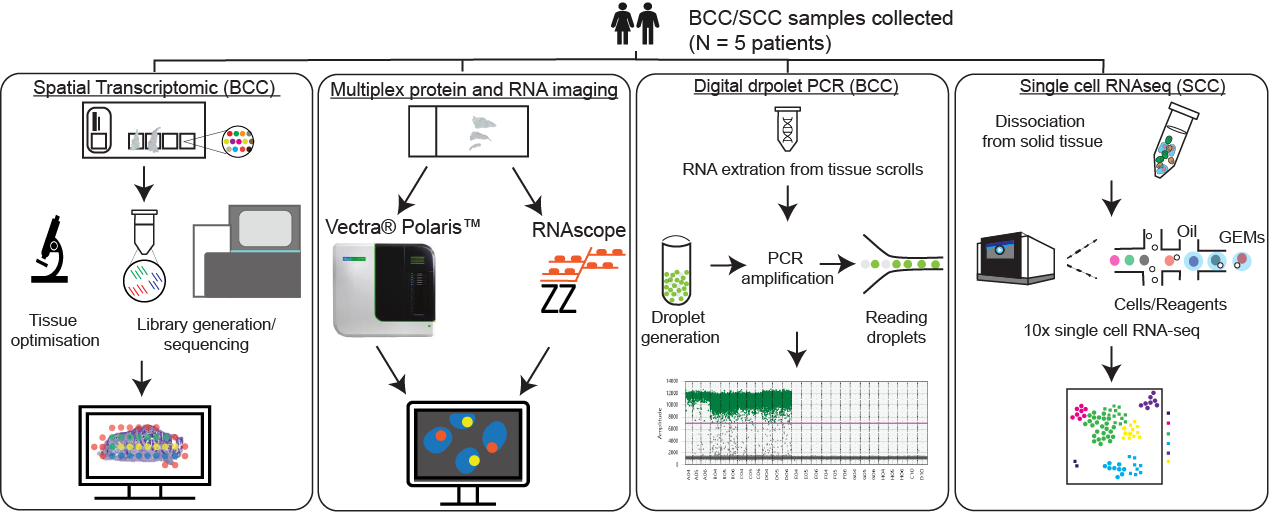
\includegraphics[width=\columnwidth]{Chapter2/Figures/Chapter2_techsum_figure1.png}
    \caption[An integrated technological and computational approach to study cell-cell interaction across the whole tissue section.]{ An integrated technological and computational approach to study cell-cell interaction across the whole tissue section. A workflow illustrating the combination of four technologies to study L-R interaction in skin cancer tissue. The generated data were used for developing STRISH.}
    \label{fig:Chap2_figure1}
\end{figure}

\begin{figure}[htp]
\renewcommand{\figurename}{Figure}
    \centering
    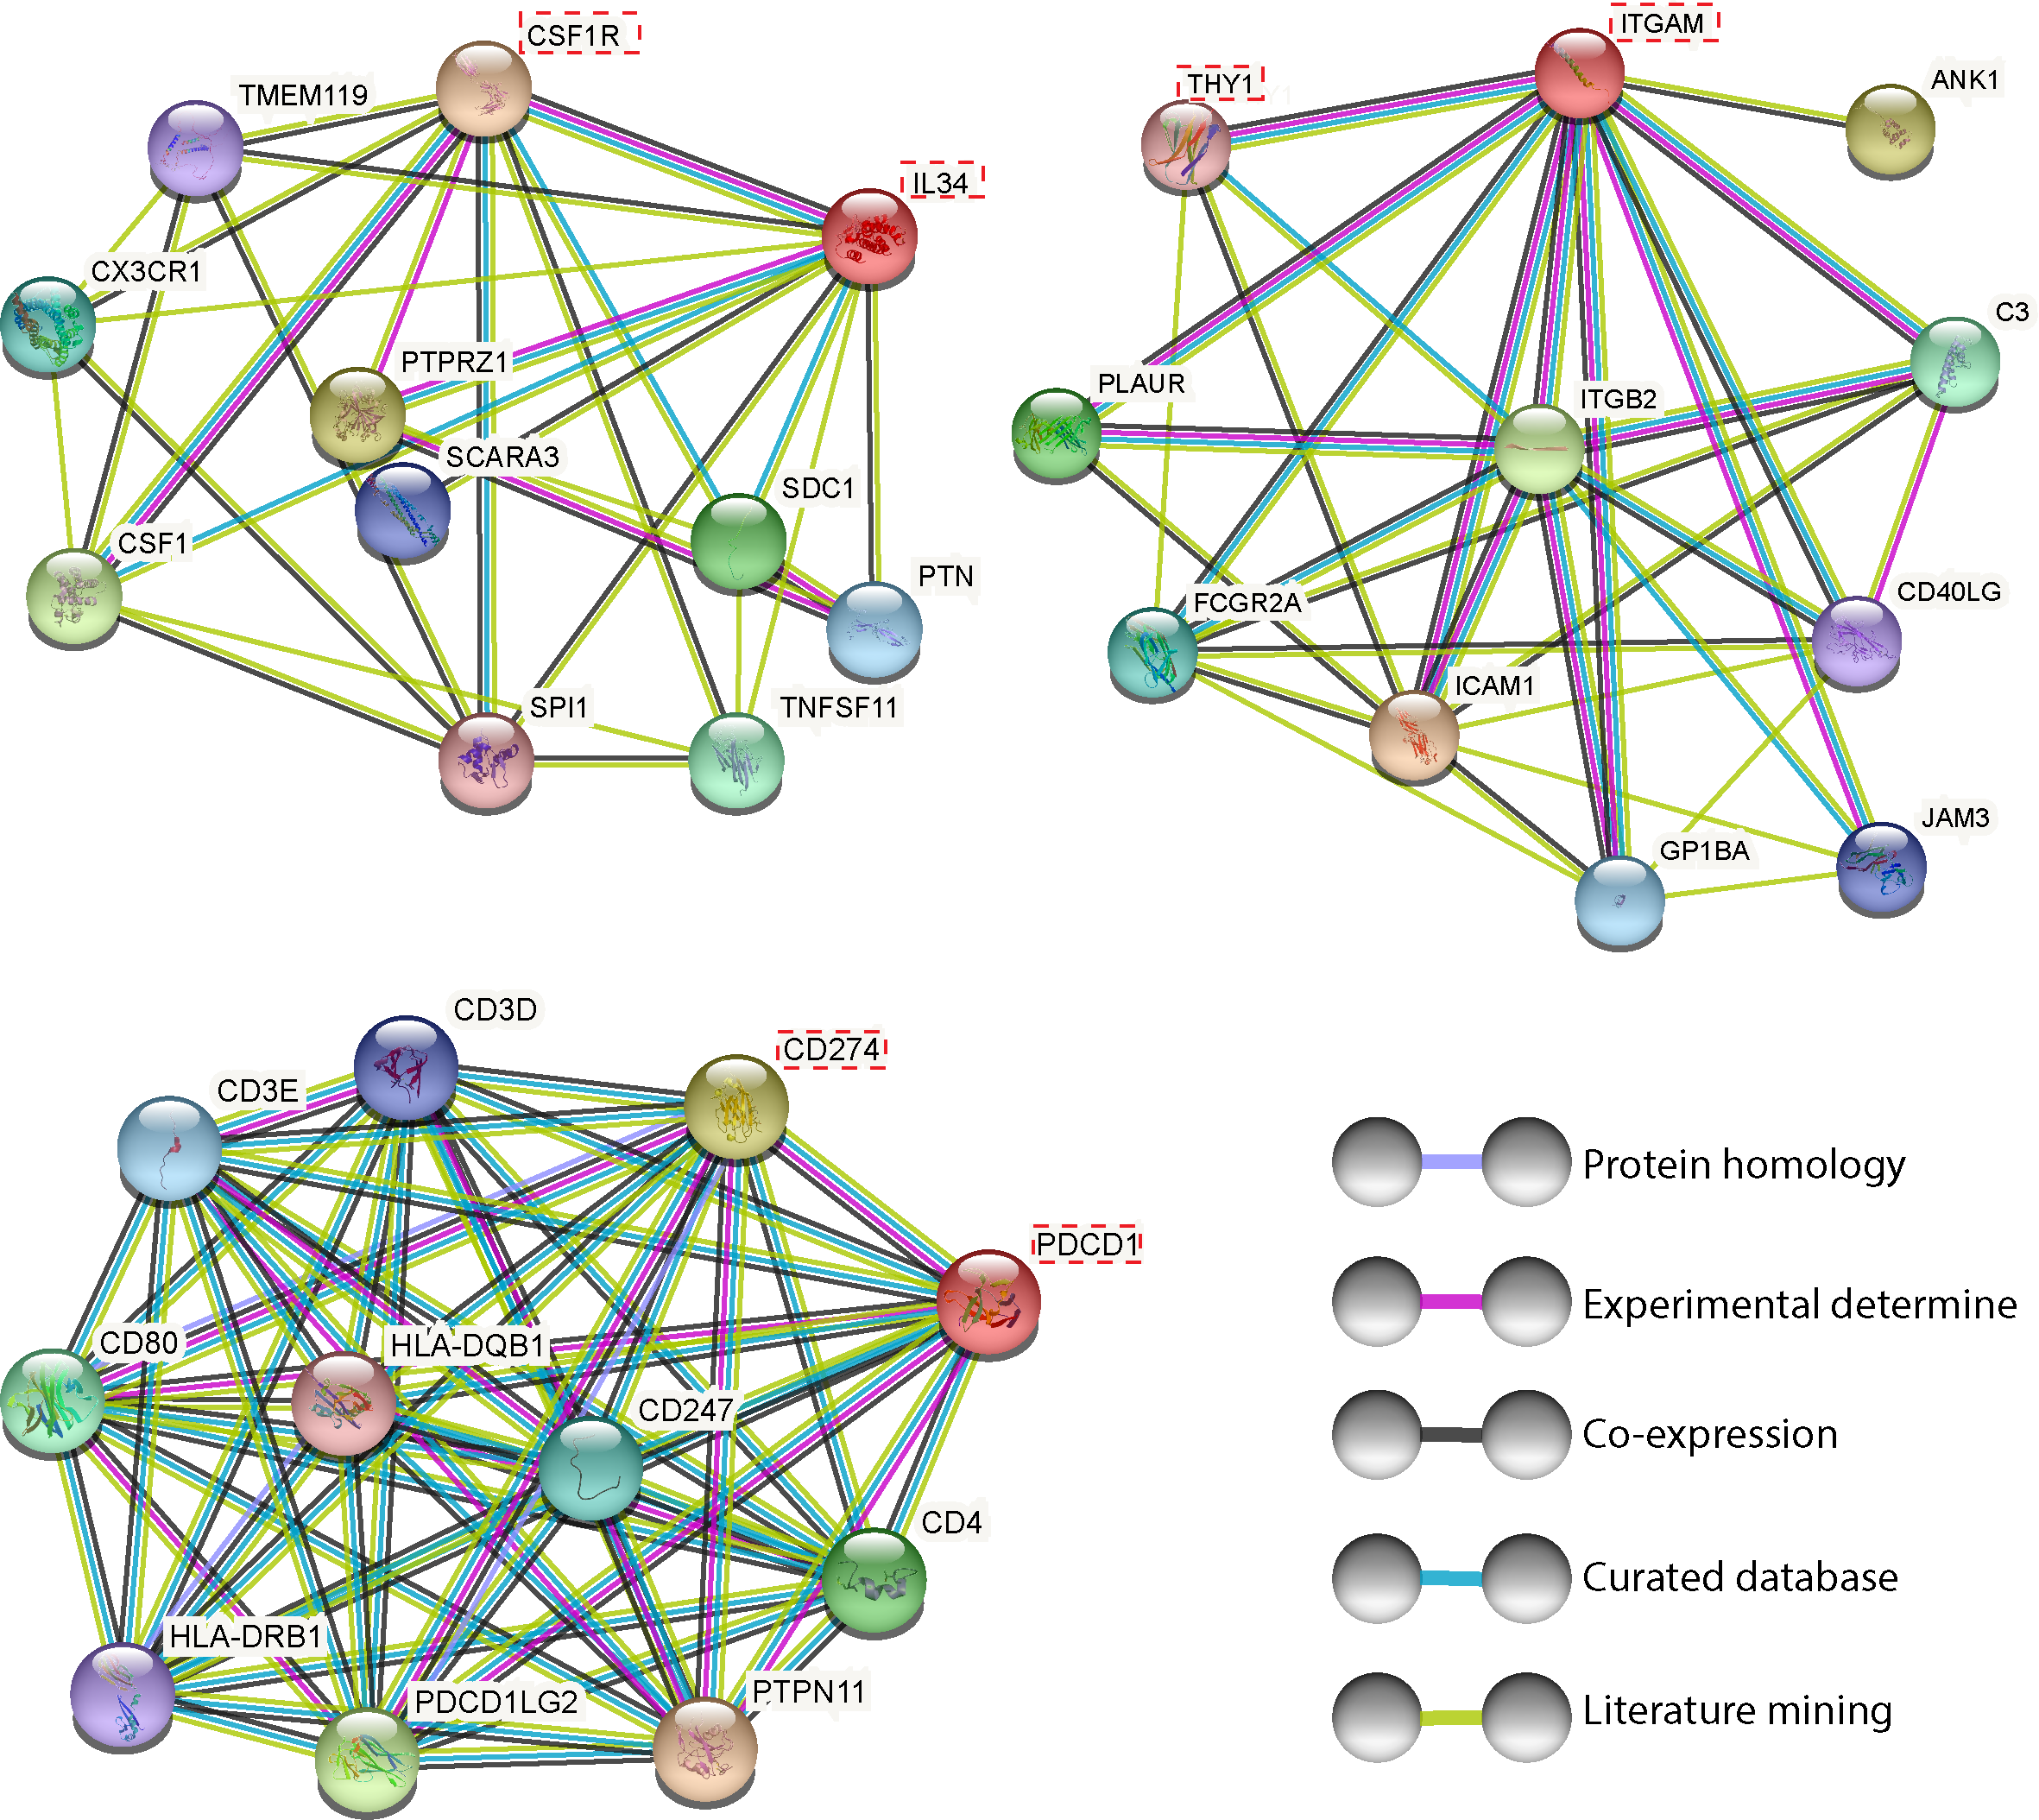
\includegraphics[width=0.66\columnwidth]{Chapter2/Figures/Supplemental_Fig_S1.png}
    \caption[Interaction networks of the 3 ligand-receptor pairs namely, CSF1R-IL34, ITGAM-THY1 and PD1-PD-L1.]{Interaction networks of the 3 ligand-receptor pairs namely, CSF1R-IL34, ITGAM-THY1 and PD1-PD-L1. Each node represents a protein and is connected to each other by multiple edges, indicating the possibility of interaction between each pair. The edges are coloured by the method which was used to determine the interaction}
    \label{fig:Chap2_Supfigure1}
\end{figure}

% ***************************************************
% \section{Data analysis methods and quantitative validation}
	%CREATE YOUR OWN LABEL.
\section{Methods}
\label{Sec:Methods}
\subsection{Inferring cell-cell interaction through ligand-receptor pairs from scRNA-seq data}
We performed scRNA-seq analysis from the cells dissociated from three tissue samples (Table \ref{table:patientInfor}). scRNA-seq measures the expression of all genes and data can be used for genome-wide prediction of cell-cell interaction (Figure \ref{fig:Chap2_figure1}). Freshly shaved suspected SCC and BCC lesions and a 4mm punch biopsy of non-sun exposed skin (Normal B18 ) from the same patient were collected for immediate tissue dissociation (Table \ref{table:patientInfor}). The 10x Genomics Chromium scRNA-sequencing followed the manufacturer’s instructions, using the Single Cell 3’ Library, Gel Bead and Multiplex Kit (version 2, PN-120233; 10x Genomics). Cell numbers in each reaction were optimized to capture approximately 3,000 cells. The single-cell transcriptome libraries were sequenced on an Illumina NextSeq500 machine. The BCL file was converted to a FASTQ file using bcl2fastq/2.17. We used CellRanger/3.0.2 for mapping to Homo sapiens. GRCh38p10 reference. 

We performed scRNA-seq data quality control following Seurat pipeline. All three gene-barcode count matrices were loaded and merged into a single SeuratObject using Seurat/4.0.0 in R/4.0. We removed cells with fewer than 200 or more than 5000 genes and cells with over 20\% of all reads mapped to mitochondrial genes. Seurat canonical correlation analysis was performed to correct the batch effect and integrate the samples. The processed expression matrix was scaled to 10,000 reads per cell and normalized, and only the top 5000 most variable genes were kept for PCA dimensionality reduction. The top 50 PCs were used to generate the UMAP plot and cluster the cells using Louvain graph-based in Seurat (Figure \ref{fig:Chap2_Supfigure2}B). Using FindClusters function with a resolution of 0.7, we determined 12 subpopulations of cell types. Finally, cell type annotation was carried out by differential expression (DE) comparison of each individual cluster against the remaining clusters. DE analysis was performed to find the top 100 differentially expressed genes for each cluster. Clusters with similar top DE genes were combined, which subsequently resulted in 3 different Keratinocytes subtypes, including KC Basal (KRT15, KRT14, CXCL14  upregulated), KC Differentiating (KRT1, 2 and 10), KC Cycle (TOP2A, STMN1)  \cite{joost2016single, ji2020multimodal} and 2 skin specific cell types Melanocyte (DCT, TYR, TYRP1), Pilosebaceous (DEFB1, DEFB2) \cite{belote2021human}. Besides, we identified three immune cell types that are commonly found in skin tissue  Lymphocyte (CD8, CD4), Myeloid (highly expressed CD207, S100A9 and HLA-DRA), Plasma Dendritic cells (CD20, CD79 upregulated) \cite{ji2020multimodal}.          

To infer cell-cell interaction through L-R pair, we applied NicheNet L-R prediction pipeline \cite{browaeys2020nichenet} on our scRNA-seq datasets of cancer and normal samples from a patient ID B18 (Table \ref{table:patientInfor}). We ran the gene differential expression analysis for two conditions, cancer and normal, to identify the genes that differentiate the two conditions. Using deferentially expressed genes, we determined the top 12 upstream ligands and then filtered the prebuilt L-R network to find the corresponding upstream receptor.

\subsection{Visium spatial transcriptomics sequencing and spatially resolved cell-cell interaction analysis}
We performed ST-seq on four tissue sections from three BCC/SCC patients (patient ID-E15, B18, F21) \ref{table:patientInfor}. Four cryosectioned tissues at $10\mu m$ thickness were transferred to chilled Visium Tissue Optimization Slides and Visium Spatial Gene Expression Slides and allowed to adhere by warming the back of the slide. RNAs extracted from the Visium were sequenced following the manufacturer’s instructions. Next, the Visium raw sequencing data in BCL format was converted to 110,782,035 FASTQ reads using bcl2fastq/2.17. The reads were trimmed by cutadapt/1.8.3 to remove sequences from poly-A tails and template-switching oligos. We used SpaceRanger to map FASTQ reads to the cellRanger human reference genome and gene annotation for GRCh38-3.0.0. On average, we mapped 94,700 reads for each spot and detected 1,428 genes. The count matrix of each Visium data was preprocessed to remove genes expressed in less than three cells, followed by the normalization, log transformation and scaling. For spot clustering, we first performed gene expression normalization using spatial morphological information from the H\&E image then clustered the spots using the Louvain community detection algorithm \cite{pham2020stlearn}. The normalization was to reduce the technical limitation in detecting lowly expressed genes. Besides, a neighbourhood graph of spots was built based on the reduced dimensional space, followed by the application of Louvain community detection to similar groups of spots into clusters. 

Regarding cell-cell interaction from ST-seq, we performed the prediction by querying the pair IL34 and CSF1R using the CellPhoneDB, Nichenet and stLearn packages \cite{pham2020stlearn, efremova2020cellphonedb, browaeys2020nichenet} (Figure \ref{fig:Chap2_figure1_result}A-C, \ref{fig:Chap2_Supfigure3}-\ref{fig:Chap2_Supfigure4}). For L-R prediction with CellPhoneDB, we applied the default parameters \cite{browaeys2020nichenet, efremova2020cellphonedb} and used a curated database v2.0.0. Additionally, similar to the scRNA-seq analysis for cell-cell communication via L-R pairs, we applied NicheNet L-R prediction on ST-seq data. The upstream ligands were ranked by descending Pearson values, and the top 5 ligands were pulled out to sort out the corresponding upstream receptors (Figure \ref{fig:Chap2_figure1_result}G).  

\subsection{Multiplexed RNA \textit{in situ} hybridization with RNAscope}
Following the whole spatially resolved transcriptome experiment, we performed a targeted capture of transcripts using RNAscope to examine the interaction through the L-R pair. Briefly, 5 tissues with each 10µm thickness tissue slide were sectioned from the optimal cutting temperature (OCT) embedded BCC or SCC tissue block was used for the \textit{in situ} hybridisation assay. The consecutive sections of each OCT block were made for the negative control. The slide was stained with a mixture of the 5 probes to allow them to hybridize with RNAs. The negative control slide was stained with RNAscope HiPlex 12 Negative control Probe that was provided in the kit. The images were captured by Axio Z1 slide scanner (Zeiss) with an appropriate adjustment of each fluorescent intensity. The first round of images was performed using 4 filters, including DAPI for nuclei.

The slide was stained with a mixture of the 5 probes to allow them to hybridize with RNAs. The negative control slide was stained with RNAscope HiPlex 12 Negative control Probe that was provided in the kit. The images were captured by Axio Z1 slide scanner (Zeiss) with an appropriate adjustment of each fluorescent intensity. The first round of images was performed using 4 filters, including DAPI for nuclei, Cy3 for THY1, Cy5 for IL34, and Cy7 for CSF1R. For the high resolution of an image, a 40x objective was used, and the Z-stack interval was set up to 1.5µm of depth resulting in 9 Z-slices for each slide. The images were further processed by ZEN software (version 3.2) for manual stitching and adjusting contrast/brightness.

\subsection{STRISH pipeline for cell-cell interaction analysis}
\label{Sec:2.3_validation} 
To automatically uncover the interaction of immune cells and cancerous cells in the whole BCC/SCC tissue sections (Table \ref{table:patientInfor}), we developed an analysis pipeline called STRISH. A standard multiplexing RNAscope which captured the cell nuclei and RNA fluorescence signal in a multidimensional image format is used as the input for the pipeline. First, we utilised stardist \cite{schmidt2018cell} model, and QuPath \cite{bankhead2017qupath} to perform cell detection. After cell segmentation, we applied the preprocessing step to calculate the mean signal values of all 9 of the Z-slices following Equation (1), which aggregates the signal from multiple Z slices into one layer. Noted that during the RNAscope imaging, the slide was scanned using Z-stack interval, which resulted in multiple slices of image. It is possible to carry out cell detection at every Z-slice image. However, stardist has consistently outperformed other models in detecting the overlapped signals from the nucleus \cite{schmidt2018cell}. Thus, it allows us to capture the cell with a single-layer image and avoid computational inefficiency. The cell detection process transforms every cell from the DAPI channel in the image into a polygonal object (a margin for the cell membrane is added to the nuclei boundary). Secondly, the mean intensity of the RNA fluorescence signal within the cell boundary was measured and assigned to the corresponding cell (Figure \ref{fig:Chap2_figure2}A Step 1). After that, STRISH provides a function to convert the whole slide image into a single-cell object called $STRISH\_Object$, which is customised from AnnData \cite{wolf2018scanpy}. 

\begin{figure}[htp]
    \centering
    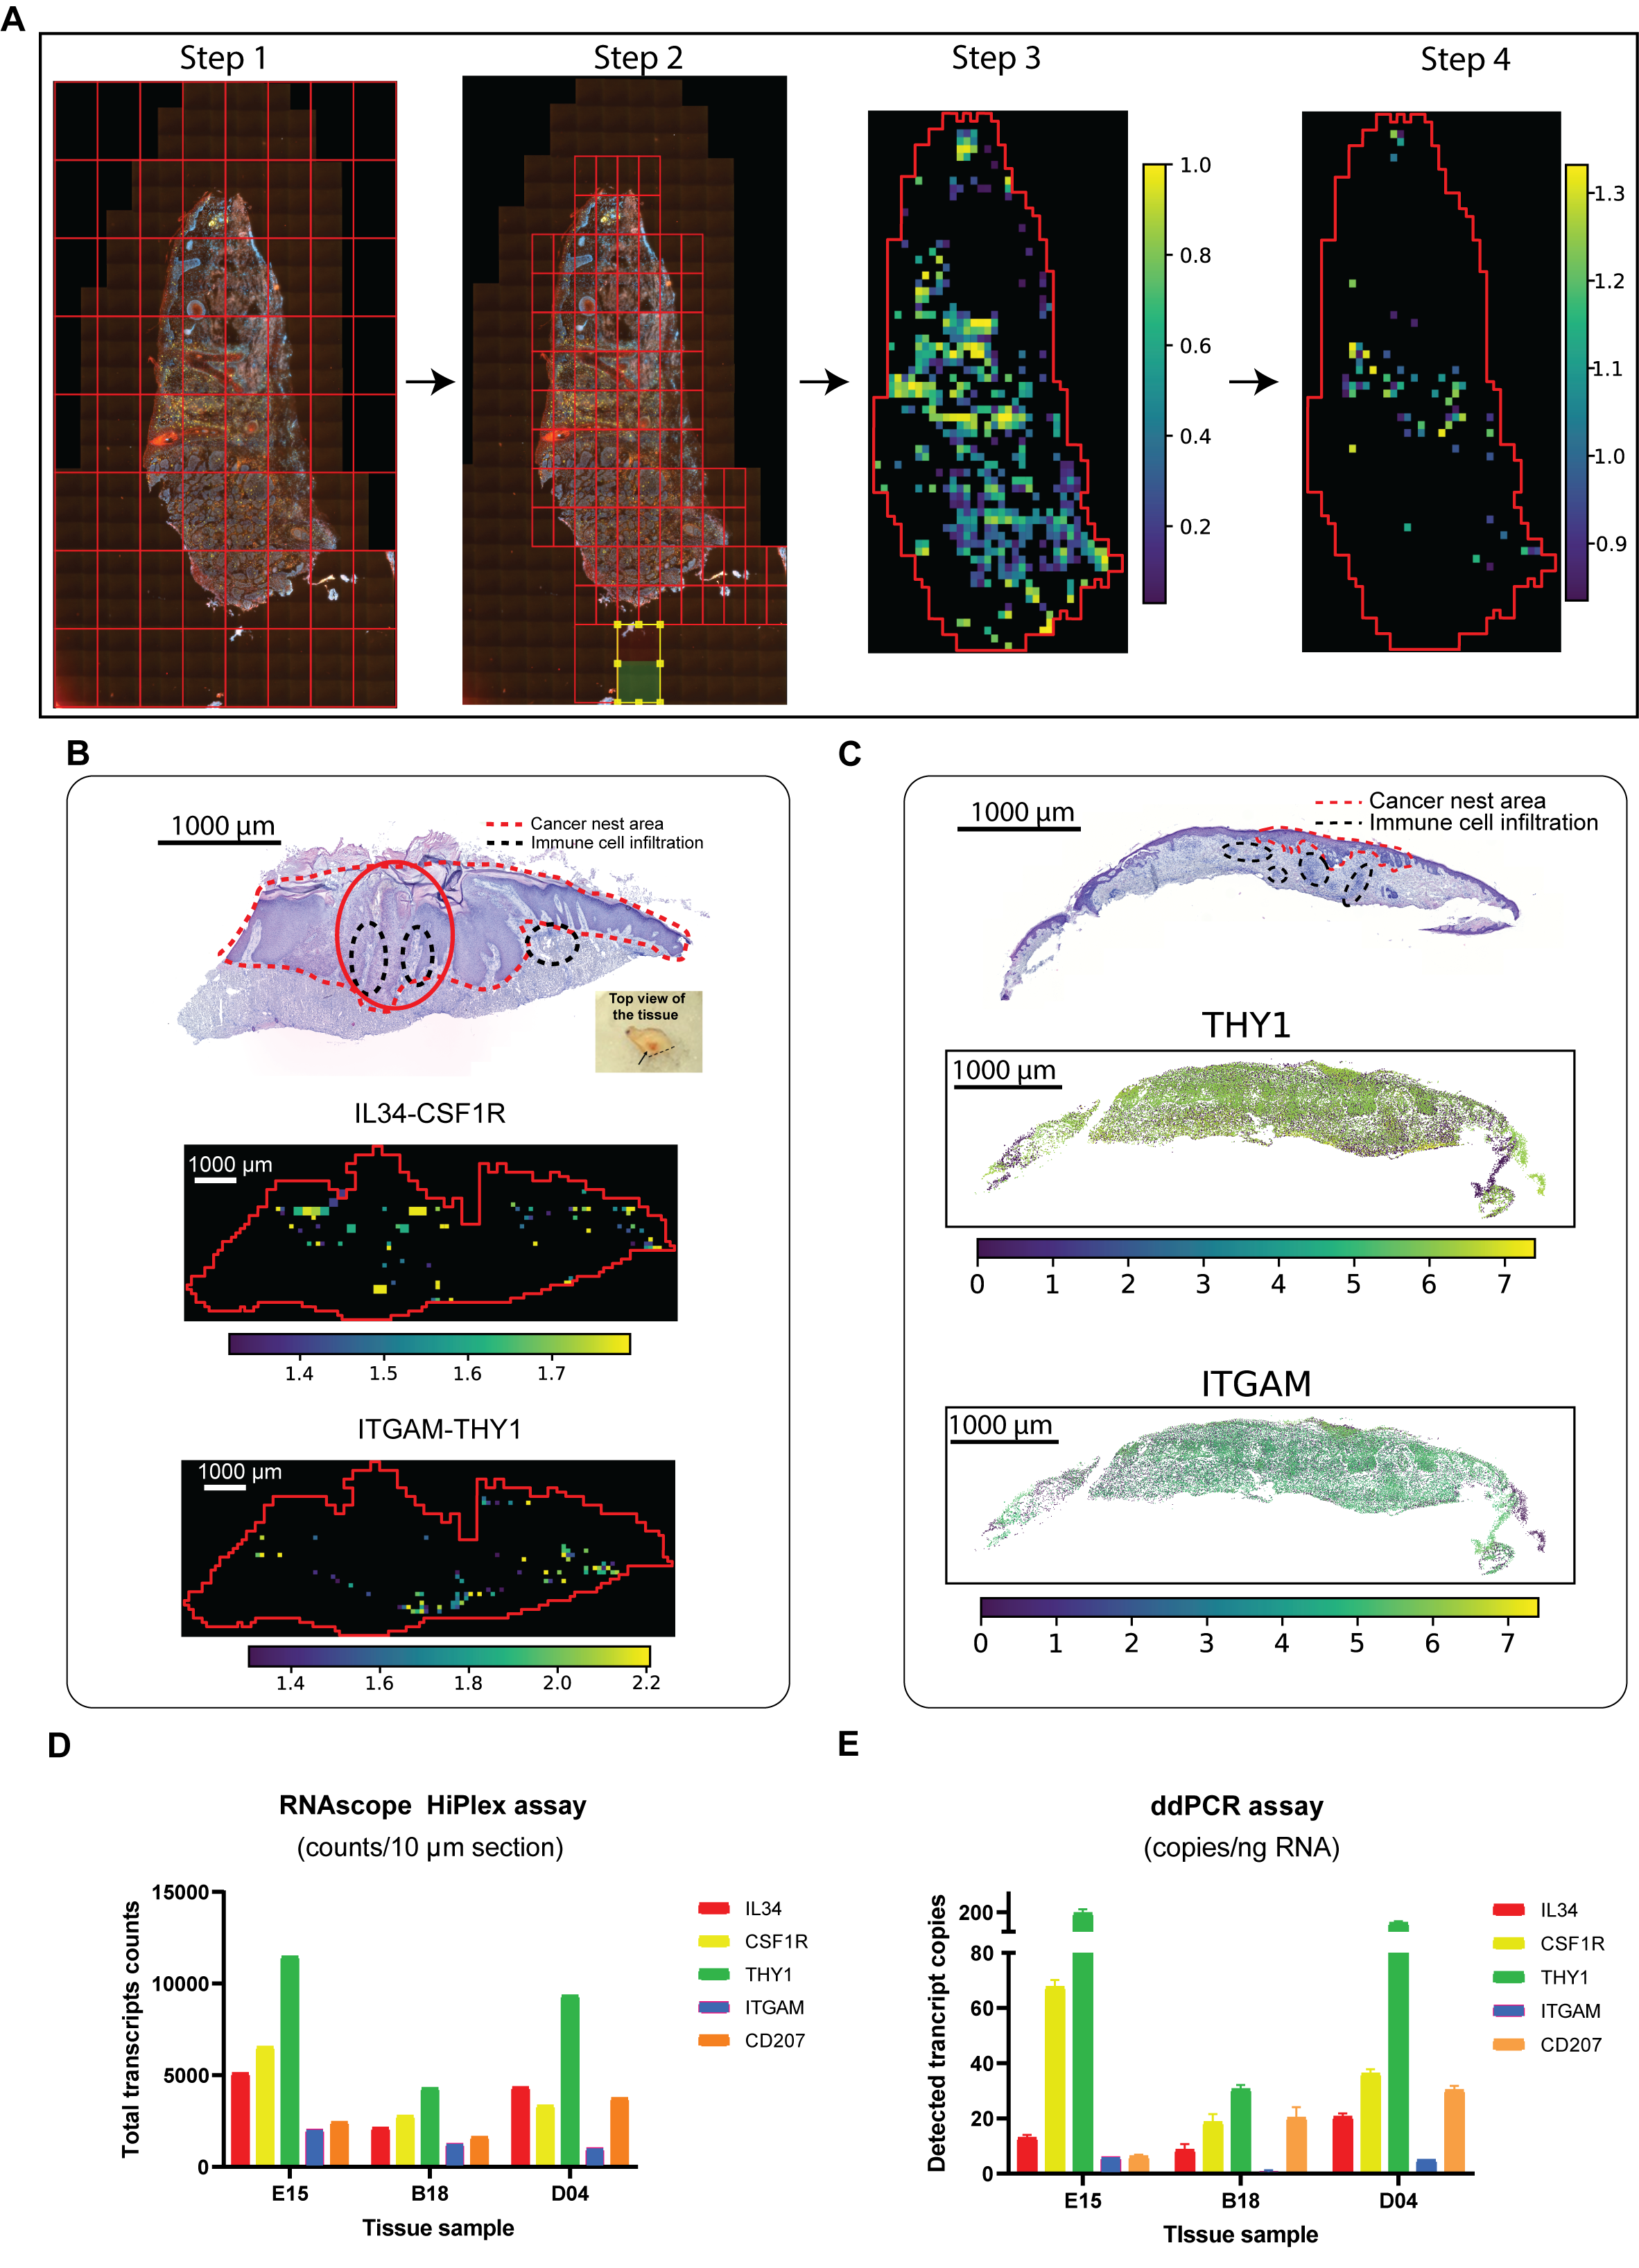
\includegraphics[width=0.95\columnwidth]{Chapter2/Figures/Chapter2_Fig2.png}
    \caption[Detection of target RNAs in skin cancer patients by collective transcriptomic and genomic methods.]{ Detection of target RNAs in skin cancer patients by collective transcriptomic and genomic methods. (A) STRISH analysis method to scan for local-coexpression of ligan-receptor pairs. Steps from raw RNAscope data to creating a tissue-scale heatmap (significant activity map) of local co-expression of target mRNAs are shown. (Legend continues on the following page.) }
    \label{fig:Chap2_figure2}
\end{figure}
\begin{figure}[t]
  \contcaption{Brifely, STRISH splits the image into large, even-size windows (Step 1). Based on cell segmentation and the count of cells per window, STRISH further splits a window into smaller ones if the window has more cells than required and discards those windows without cells (Step 2). Using the remaining windows, which contain cells expressing L-R, STRISH can perform the co-localization scoring and statistical test to produce a heatmap of the most significant windows in a spatial context (Steps 3 and 4). (B) From top to bottom: annotated H\&E of SCC patient ID-F21 and the corresponding heatmaps (activity maps) of local co-expression for the two L-R pairs, IL34-CSF1R and THY1-ITGAM, respectively. (C) The expression levels of THY1 and ITGAM using RNAscope signal measurement within the cells throughout the tissue of the patient ID-D04. (D) and (E) The absolute copy number of the target mRNAs counted using ddPCR and RNAscope assays.}% Continued caption
\end{figure}

\begin{equation}
c_{i} = \frac{\sum_{j=1}^{n_{slides}}(c_{ij})}{n_{slides}}
\label{chap2:eq:01}
\end{equation}
where $c_i$ indicates the DAPI or RNA marker channel and $j$ is an iterator of the Z-slices.

Finally, several data preprocessing functions are available within STRISH to remove the effect of artificially high background from fluorescent intensity (outlier) and cells that are too large or small (false detection). By default, STRISH clips that cell’s marker expressions to 95th percentile of all intensities and remove cells that are too small (less than 5th percentile of all areas). To determine more specific thresholds, STRISH enables several functions for quality control and plotting the marker expression of every cell (\ie Fig \ref{fig:Chap2_figure2}C).

\begin{equation}
    coexpression\_sc_{wi} = \begin{cases}
    \frac{n_{cell\_ligand_{wi}} + n_{cell\_receptor_{wi}} }{n_{total\_cell_{wi}}}&;\text{if $ n_{cell\_ligand_{wi}} \neq 0$ and $n_{cell\_receptor_{wi}} \neq 0$}\\
    0              & ;\text{if $ n_{cell\_ligand_{wi}} = 0$ or $n_{cell\_receptor_{wi}} = 0$}
    \label{chap2:eq:02}
\end{cases}
\end{equation}

To quantitatively measure the local co-expression of each window, we defined a scoring function to score the number of cells that express either ligand or receptor in the same window following the Equation \ref{chap2:eq:02}. The co-expression score considers the frequency of the cell that expressed the ligand and receptor residing in each window. Besides, the coexpression score is constrained to the presence of both marker ligand and receptor in the same window, which increases the likelihood of interaction between cells through that pair of L-R (Figure \ref{fig:Chap2_figure2}A Step 3). 
   
The downstream analysis for detecting cell local co-expression by window scanning in STRISH is summarised in Algorithm \ref{Chap2:Alg:01}. More specifically, the STRISH functionality for cell local co-expression was developed to iteratively scan through the image, using a neighbourhood window detection strategy to find the target regions with cells expressing the marker of interest. First, a cell scanning windows process is initiated to cover a broad area of scanning with dimensions for width and height set to a predefined rate of the whole scan images. While iterating through the stack of all the existing windows, STRISH will discard those windows with fewer than two cells (cell count is based on DAPI signal). For each window where the number of detected cells is greater than a threshold (user’s defined threshold depending on cancer tissue types), STRISH further splits it into smaller windows (the default rate is 50\% of the current considering window dimension) and adds these smaller windows into the iteration stack (Figure \ref{fig:Chap2_figure2}A Step 2). Finally, windows that pass the cell threshold check are subjected to the next step to detect co-expression. Using the expression level of each marker for every cell as the features, STRISH performs cell classification through standard single-cell cell clustering (\ie Leiden clustering from scanpy \cite{wolf2018scanpy}) and/or signal gating on respective marker signal.

\makebox[\linewidth]{%
\begin{minipage}{\dimexpr\linewidth}
\begin{algorithm}[H]
\SetAlgoLined
\SetKwInOut{Input}{input}
\SetKwInOut{Output}{output}
\Input{$cell\_segmentation\_file$ \CommentSty{\#cell segmentation and biomarker signal measurement result}, \newline 
$scan\_image\_fn$ \CommentSty{\#microscopy image for analysis}, \newline
$threshold$ \CommentSty{\#theshold for cell count per window} }
\Output{$cell\_colocalised$  \CommentSty{\#dataframe of cells colocalised by target ligand-receptor pair}}
	$cell\_segment\_data = read\_cell\_detection(cell\_segmentation\_file)$\;
	$scan\_img\_data = read\_img(scan\_image\_fn)$\;
	$init\_windows = add\_window\_to\_image(scan\_img\_data.shape)$\;
	$cell\_count = window\_cell\_detect(init\_windows, cell\_segment\_data)$\;
	\While{$init\_windows.count() > 0$ or $count\_cell > threshold$ }{
	$windows\_available = get\_all\_windows()$\;
	\For{$window~\in~windows\_available$}{
	$count\_cells = window\_cell\_detection(dapi\_channel, window)$\;
	\uIf{$count\_cells \leq 2$}{
	    \CommentSty{\#Remove the windows with less than 2 cells as there is no possible multiple cells interaction}\\
	$windows\_available.remove\_window(window)$\; 
	\uElseIf{$count\_cells >2$ and $count\_cells \leq threshold$}{
        \CommentSty{\#Run cell detection with respect to other marker channels}\\
        $cells\_express\_ligand = run\_cell\_detection(ligand\_channel)$\;
    	$cells\_express\_receptor = run\_cell\_detection(receptor\_channel)$\;
    	$return\_to\_file(count\_cells, cells\_express\_ligand, cells\_express\_receptor)$\;
    	$windows\_available.remove\_window(window)$\;
    }
    \Else{
        \CommentSty{\#Number of cells in current window greater than the threshold, split the window into smaller windows}\\
        $new\_windows = add\_annot\_windows(widow\, subset_rate)$\;
   \CommentSty{\#Remove the current window as the new subset windows are spawned from and replace the current window }
        $windows\_available.remove\_window(window)$ \;
    }
	}
	}
	}

 \caption{Cell detection by window scanning throughout the tissue section}
 \label{Chap2:Alg:01}
\end{algorithm}
\end{minipage}
}
To quantitatively measure the local co-expression of each window, we defined a scoring function to score the number of cells that express either ligand or receptor in the same window following the Equation \ref{chap2:eq:02}. The co-expression score considers the frequency of the cell that expresses the ligand and receptor residing in each window. Besides, the coexpression score is constrained to the presence of both marker ligand and receptor in the same window, which increases the likelihood of interaction between cells through that pair of L-R (Figure \ref{fig:Chap2_figure2}A Step 3). Once every window is scored, a statistical test for the most significant windows is used.

\subsection{Statistical test for tissue regions with significant L-R colocalization}
To validate the test for the significance of the cell-cell interactions based on colocalization scored among all the positive windows, STRISH performs the statistical test to compare the level of co-localisation of the pair of L-R of interest with the random combination of two pairs of markers available for the same window and across all the positive windows. Briefly, STRISH finds tissue locations (windows) that have coexpression of L-R pairs higher than random expression in other windows and by other non-L-R pairs. There are two randomization procedures, testing for the expression level relative to random non-L-R pair at one location (one window) and testing for significant expression of one of co-localisation of L-R pair relative to all locations a window (equation \ref{chap2:eq:03}). Firstly, the means of cell co-localisation for both ligand or receptor within every window $w_i \neq 0$ is compared to the random combination of two positive ligands and a target non-receptor marker from the same window. The comparison between real pairs of L-R cell co-localisation with the matched randomized pairs allows us to show a test for if there is a significantly more abundant presence of the cells expressing  the ligand and receptor within a window than cells co-expressing random pairs. Secondly, for all the windows that have the positive mean of the co-localisation score of the same L-R, we tested if certain windows were tested against each other to identify the significantly more cells co-expressing the pair than the remaining  most significant windows across the tissue. This test reduces false positive detection because while the scanning windows approach could capture the region of colocalisation of cells expressing the ligand and receptor, the colocalisation can be a random expression of the pairs that happened to be in the same window but were at a low level of cells can also be at random. The second randomness test aims to identify the windows which have the highest frequency of colocalisation of the target L-R compared with all other windows throughout the tissue. The combination of two statistical tests generates will provide a P value for each window which corresponds to either significant or insignificant colocalisation. We developed a Python-based pipeline to construct the heatmap of cell local co-expression from the final p-value of the significant windows. 
\begin{equation}
    P_{wi} = \frac{\sum_{i=1}^{m}(coexpres\_sc_{wi} > coexpres\_sc_{random\_pairs_{wi}})+ \sum_{j=1}^{n-1}(coexpres\_sc_{wi} > coexpres\_sc_{pos\_lr_j}) }{total\_random_{random\_pairs} + total\_window_{pos\_lr}}
    \label{chap2:eq:03}
\end{equation}
Where,	$coexpres\_sc_{wi}$  is the colocalisation score of each window $w_i$, calculated as in Equation \ref{chap2:eq:02}, ($m$ is the number of windows in the dataset); $coexpres\_sc_{random\_pairs_w}$ is the colocalisation score of the same window $w_i$, calculated for random pairs of other markers in the dataset that are known to not interact, as calculated in Equation \ref{chap2:eq:02}; the number of random pairs is the permutation of $\frac{(n*(n-1))}{2}$ (where n is the number of markers in the dataset); $coexpres
\_sc_{pos\_lr_j}$is the colocalisation scores of all the windows within the tissue that express the same ligand and receptor pair as in $w_i$; $total\_random_{random\_pairs}$ denotes the total number of windows with randomized pairs of markers; $total\_window_{pos\_lr}$  denotes the number of windows with the same pair of target ligand-receptor

\makebox[\linewidth]{%
\begin{minipage}{\dimexpr\linewidth}
\begin{algorithm}[H]
\SetAlgoLined
\SetKwInOut{Input}{input}
\SetKwInOut{Output}{output}
\Input{$target\_lr$ \CommentSty{\#pair of target ligand receptor}, \newline 
$random\_pair\_markers$ \CommentSty{\#random pair of ligand receptor}, \newline
$windows\_available$ \CommentSty{\#list of windows with cell colocalisation }, \newline
$p\_threshold $ \CommentSty{\#threshold for statistical significant testing}}
\Output{$sig\_windows$  \CommentSty{\#list of windows with significant level of lr colocalisation}}
	$target\_lr, random\_pair\_markers, window\_available, p\_threshold = input()$\;
    $coexpres\_sc\_lr = cal\_coexpress(window\_available, target\_lr) $\;
    $coexpres\_sc\_random = cal\_coexpress(window\_available, random\_pair\_markers)$\;
    $window\_sc\_all = concatenate(coexpres\_sc\_lr, coexpres\_sc\_random)$\;
    $all\_window\_pos\_target\_lr = window\_score\_all[target\_lr]$\;
	\For{$window~\in~window\_sc\_all $}{
	    $window\_coord = current\_window.location()$\;
	    $current\_lr\_pair\_scores = current\_window[target\_lr]$\;
    	$random\_pair\_sc = current\_window [window\_coord, random\_pair\_markers]$\;
    	$merged\_background\_sc = merge(random\_pair\_sc, all\_window\_pos\_target\_lr)$\; 
    	$total = sum(current\_lr\_pair\_sc >= merged\_background\_sc)$\;
    	$current\_window\_Pvalue = total / len(merged\_background\_sc)$\;
    	$window\_sc\_all[target\_lr\_Pvalue] = current\_window\_Pvalue$\; 
     	$window\_sc\_all[target\_lr\_log\_Pvalue]= -log10(window\_sc\_all)$\; 
	}
	$sig\_windows = window\_sc\_all[window\_sc\_all[target\_lr\_Pvalue] > p\_threshold]$\;
 \caption{Quantifying local co-expression and statistic test }
 \label{Chap2:Alg:02}
\end{algorithm}
\end{minipage}
}

As there were two rounds of RNAscope imaging, we added to STRISH an image registration functionality. For the interaction of ITGAM and THY1, as the signals of the genes were captured in two separated imaging rounds with the respective stitching in post-process, some variants were introduced (Figure \ref{fig:Chap2_Supfigure7}A-B). To overcome the unaligned tissue layout, we performed image registration to map one image to the other (Figure \ref{fig:Chap2_Supfigure7}C). The image registration is performed solely using SITK library \cite{lowekamp2013design, yaniv2018simpleitk}.  

\begin{figure}[ht]
\renewcommand{\figurename}{Figure}
    \centering
    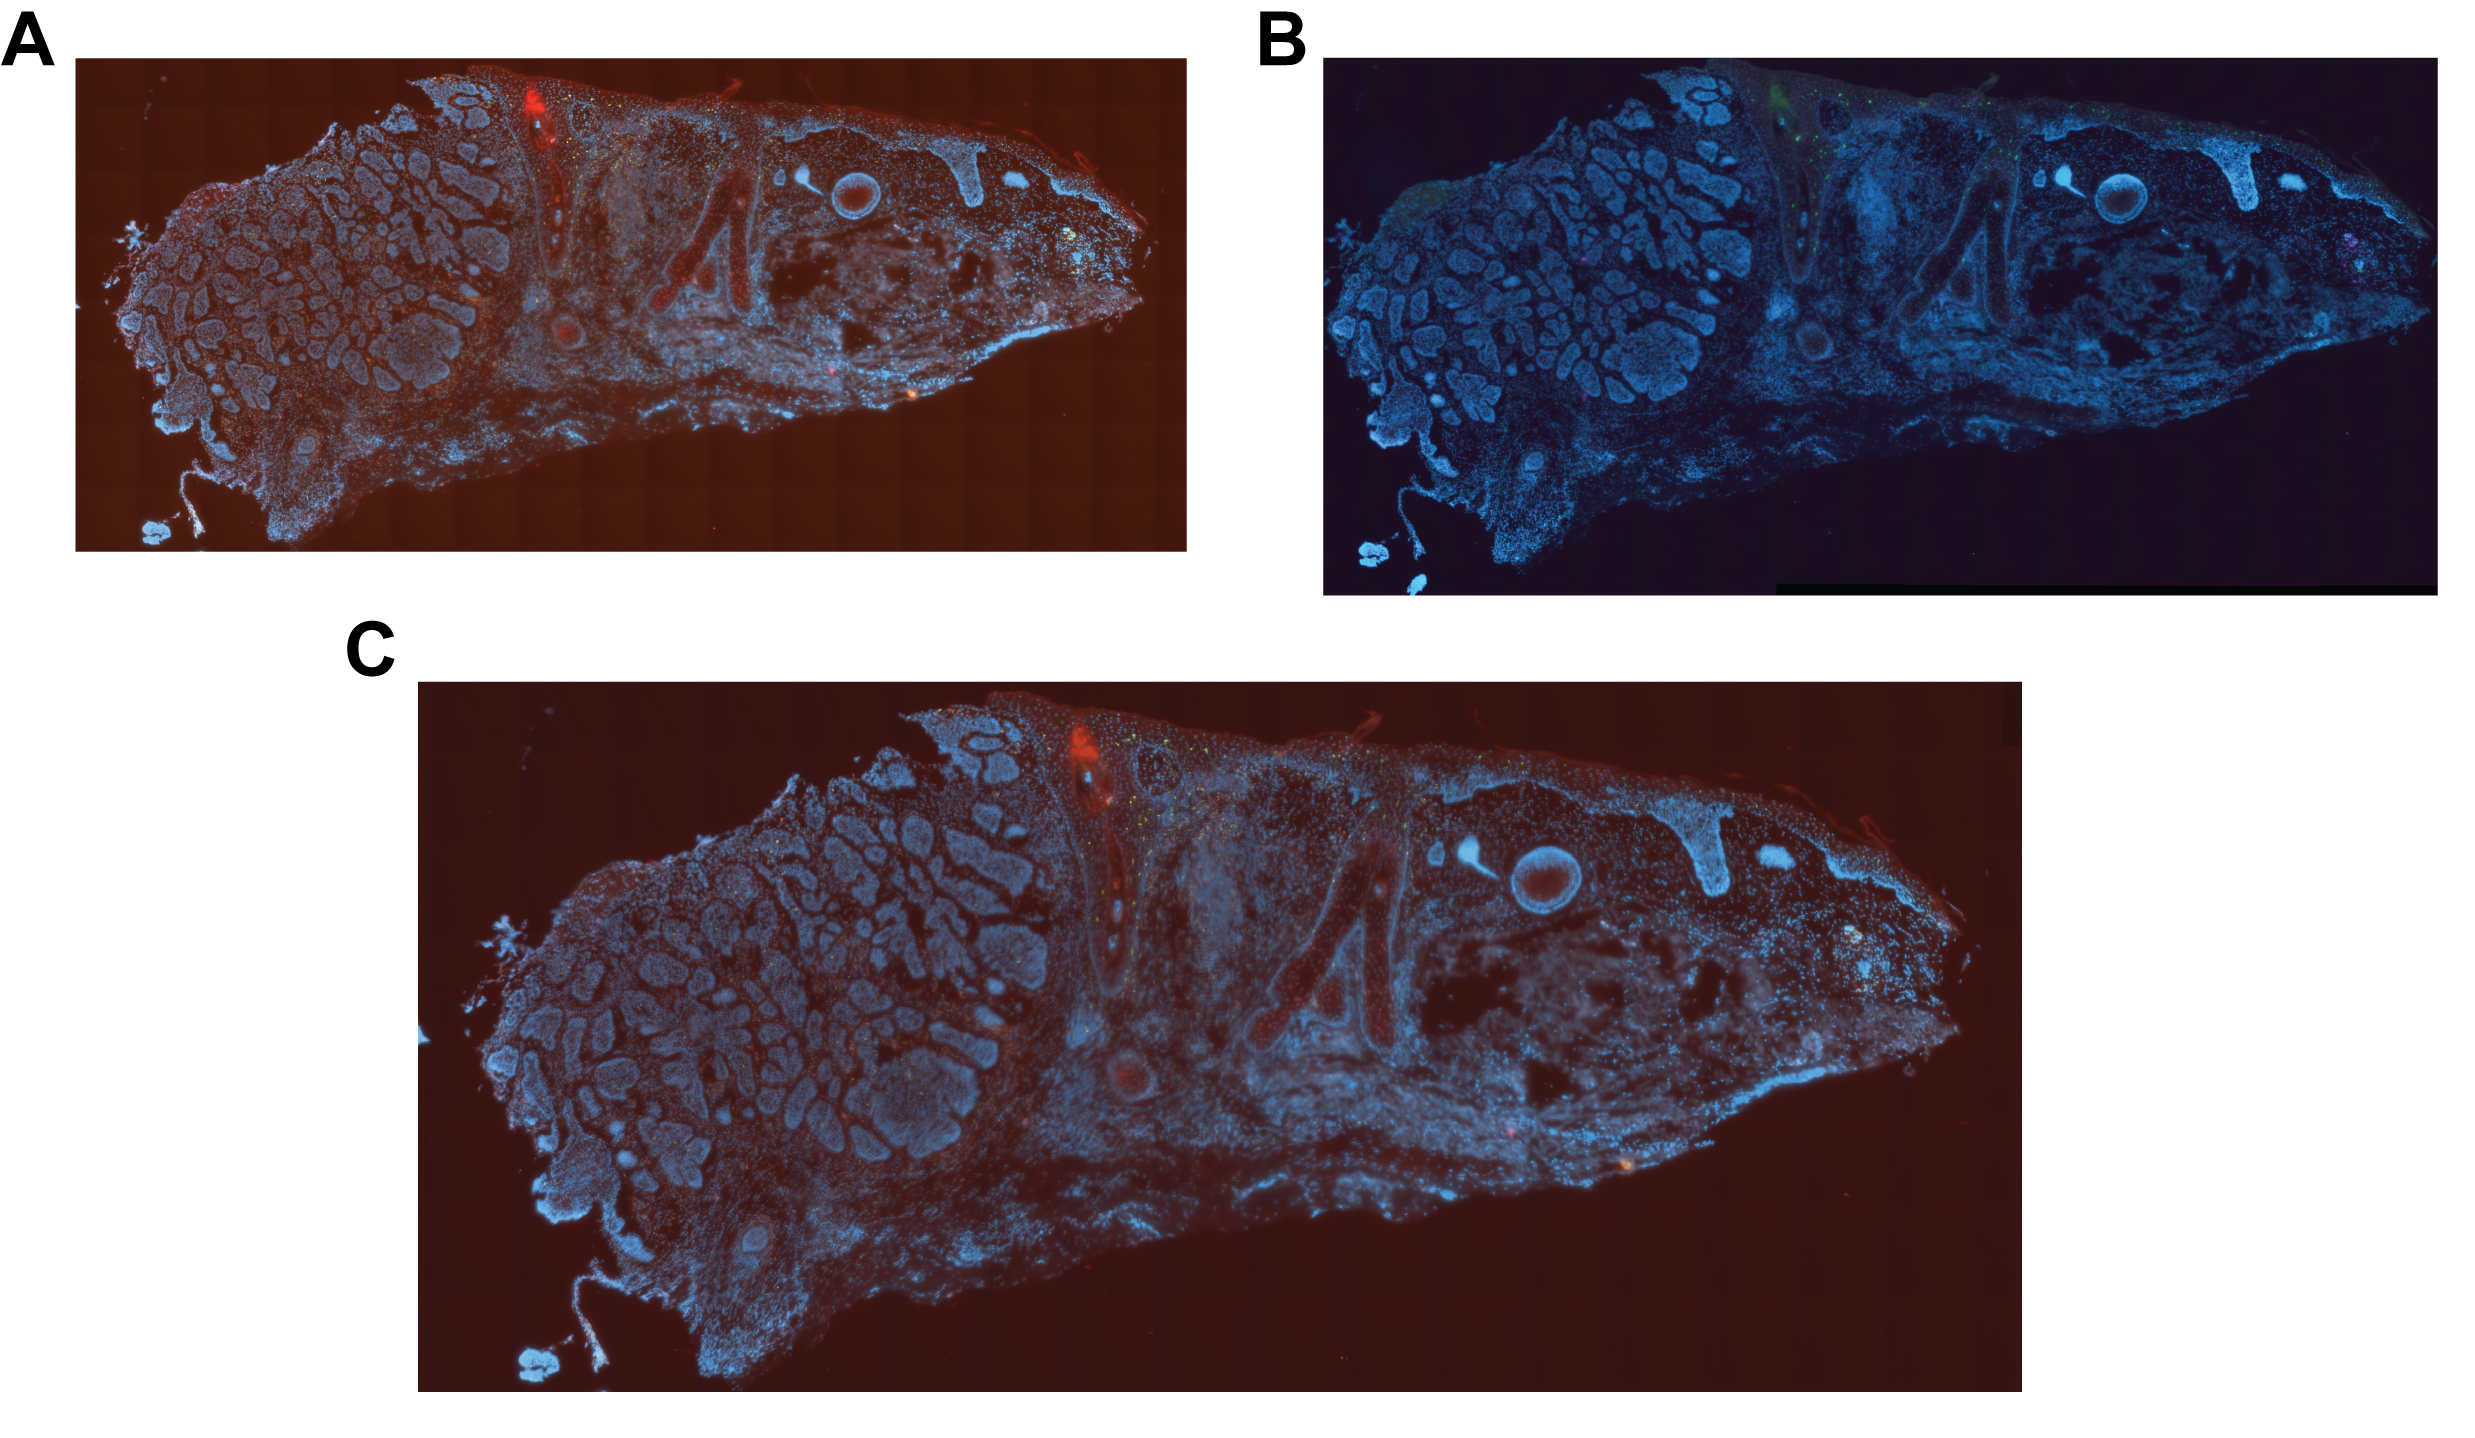
\includegraphics[width=0.75\columnwidth]{Chapter2/Figures/Supplemental_Fig_S7.png}
    \caption[Outputs from two steps in the STRISH analysis pipeline for RNAscope images registration.]{Outputs from two steps in the STRISH analysis pipeline for RNAscope images registration. (A) The RNAscope image for THY1, IL34, and CSF1R signals from the first round of imaging. (B) The RNAscope image for ITGAM and CD207 signals from the second round of imaging (for the same tissue section). (C) The result of image registration combines the outputs from the two imaging rounds. After registration, the results from the two hybridization rounds (\ie THY1 and ITGAM) were compatible with the local co-expression analysis.}
    \label{fig:Chap2_Supfigure7}
\end{figure}

Our code for detecting local co-expression of L-R pairs, generation of the heatmap (interaction activity map), and tissue plotting with contour marking tissue boundary are publicly available on GitHub and STRISH package is available on PyPi. 

% \subsection{Extending STRISH for analysis of Vectra Polaris mutiplex protein data}
% In addition to the analyses at transcriptomic level (RNAscope data), we also extended STRISH’s applications to quantify the interaction between cells at protein level. We reasoned that the STRISH pipeline is computationally flexible and could be applied to construct the landscape of L-R interaction at protein level. Similarly, the analysis on RNAscope, STRISH first performed cell detection by applying positive cell detection on the image that was generated from the Vectra Polaris system. Subsequently, the pipeline applied the PD-1 and PD-L1 markers detection and thresholding to the windows containing fewer than 100 cells. Finally, the STRISH min-max normalization was performed and a heatmap was plotted to display the local co-expression levels of PD-1 and PD-L1.  
% ***************************************************

\section{Detecting cellular communication from transcriptome-wide scanning to targeted interaction validation}
\label{Sec:2.2_CCC_ST}	%CREATE YOUR OWN LABEL.
\subsection{Genome-wide analysis of ligand-receptor interaction using scRNA-seq data}
% \subsection{Single cell RNA sequencing data analysis}
\begin{figure}[htp]
\renewcommand{\figurename}{Figure}
    \centering
    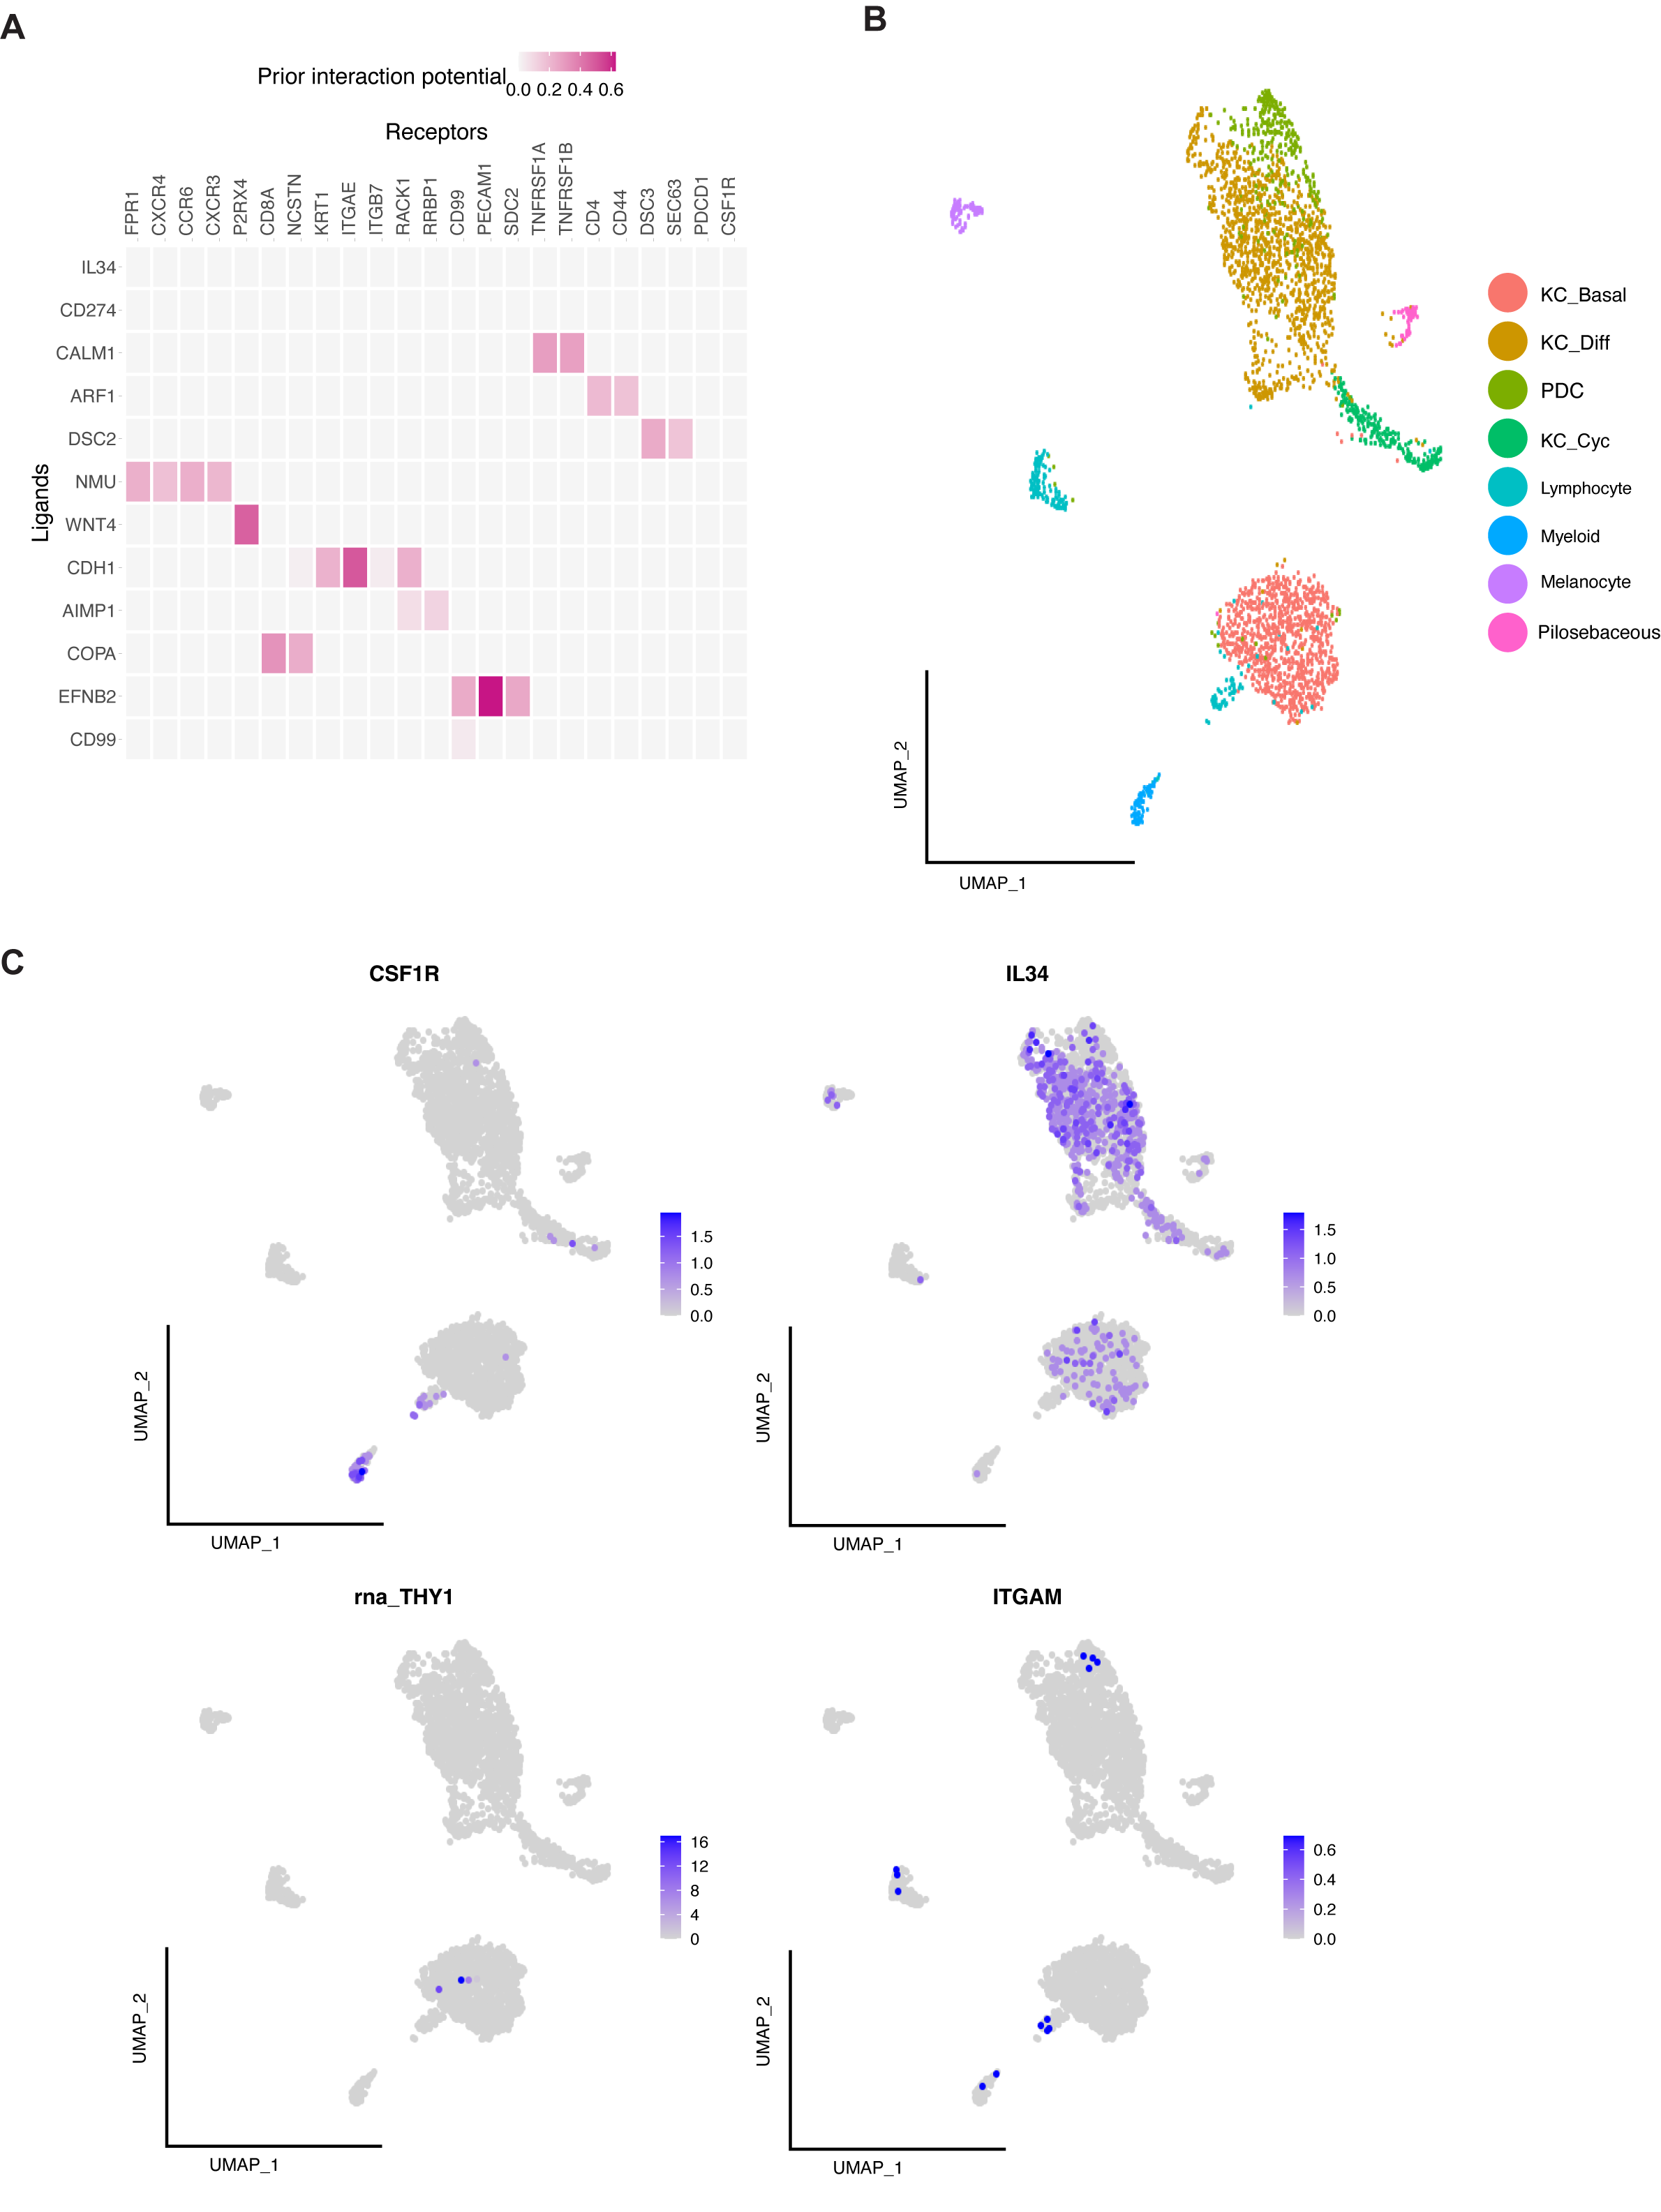
\includegraphics[width=0.75\columnwidth]{Chapter2/Figures/Supplemental_Fig_S2.png}
    \caption[scRNA-seq ligand-receptor interaction analysis of SCC cancer patient sample. ]{scRNA-seq ligand-receptor interaction analysis of SCC cancer patient sample. (A) NicheNet analysis results, with a heatmap showing ligand-receptor, predicted interaction potential for the top 12 ligands. (B) A UMAP plot with cells grouped into 14 clusters using Louvain algorithm and gene expression. Each cluster is shown as one colour. One dot represents a cell. (C) A feature plot highlighting (navy dots) the distribution of cells expressing IL34 (left plot) and CSF1R (right plot). (D) A feature plot highlighting the distribution of cells expressing THY1 and ITGAM. Cells without expression appear as grey dots.}
    \label{fig:Chap2_Supfigure2}
\end{figure}

Unsupervised clustering and differential expression analysis revealed 3 major subpopulations of epithelial (accounted for 80\% of the total cell population), including Keratinocyte (KC) Basal, KC Differentiating (KC-Diff) and KC Cycling (Methods, Figure \ref{fig:Chap2_Supfigure2}). Several immune and skin-specific cell types were also identified, including Lymphocyte, Myeloid, Dendritic, and Melanocyte (\ref{Sec:Methods}, Figure \ref{fig:Chap2_Supfigure2}). To infer potential L-R pairs that are likely used as means of intercellular communication, we applied common single-cell inference methods, CellPhoneDB \cite{efremova2020cellphonedb} and NicheNet pipeline \cite{browaeys2020nichenet} on our scRNA-seq dataset of matched samples, containing a squamous cell carcinoma sample tissue (SCC)  and a normal sample tissue from the same patient (Figure \ref{fig:Chap2_Supfigure2}A). NicheNet combines expression data with prior knowledge of gene signalling and gene regulatory networks to predict L-R pairs used by interacting cells (sender and receiver cells).  Using NicheNet differential expression analysis, we identified the list of genes associated with the L-R signalling and plotted the heatmap of potential interaction in  Figure \ref{fig:Chap2_Supfigure2}A. We expected to use the detection of known IL34-CSF1R \cite{lin2008discovery} and THY1-ITGAM \cite{wetzel2004human} interaction to assess the sensitivity of the inference approach using scRNA-seq. The two pairs were not among the significantly detected pairs predicted by NicheNet (Figure \ref{fig:Chap2_Supfigure2}A). To examine the relatedness of cells coexpressing the L-R pairs, we visualise L-R expression relative to cell cluster information in the UMAP space (Figure \ref{fig:Chap2_Supfigure2}B-C). We found evidence of KC-Basal and KC-Diff cells that expressed IL34 while the receptor CSF1R was expressed by Myeloid and Lymphocyte (Figure \ref{fig:Chap2_Supfigure2}C). However, THY1 and ITGAM were only expressed by a few cells with no distinct patterns of coexpression (Figure \ref{fig:Chap2_Supfigure2}C). The results from examining THY1-ITGAM suggested the insensitivity of using scRNA-seq alone to study cell communication. Overall, we found that scRNA-seq can be utilized to study cell communication, but statistical test based on gene expression alone has low sensitivity and mis-detects expected interactions.  

\subsection{Genome-wide analysis of ligand-receptor interaction using ST-seq}

We postulated that cell-cell communication could be more accurately assessed by using ST-seq, which preserves neighbourhood information of interacting cells. We performed ST-seq on four tissue sections from four patients, with 2xSCC and 2xBCC tissue sections, (Table \ref{table:patientInfor}), (Figures \ref{fig:Chap2_figure1_result}C, \ref{fig:Chap2_figure1_result}E, \ref{fig:Chap2_Supfigure3}A, \ref{fig:Chap2_Supfigure4}A-C, \ref{fig:Chap2_figure1_result}A).  With ST-seq protocol, hematoxylin and eosin (H\&E) image allowed us to annotate cancer and immune cells, where the morphology revealed important tissue regions, including cancer nests, immune infiltration and non-cancer regions (Figures \ref{fig:Chap2_Supfigure4}A-C,\ref{fig:Chap2_figure1_result}A ). Additionally, adjacent tissue sections were used for RNAscope analysis as a means of validation (Figure \ref{fig:Chap2_figure1_result}A, \ref{fig:Chap2_figure1_result}B;  Figure \ref{fig:Chap2_Supfigure5}).  From the same block, one section was used for ST-seq and another for RNAscope and comparing the ST-seq and RNAscope results for the two sections allows us to validate the ST-seq prediction data (Figures \ref{fig:Chap2_Supfigure3}, \ref{fig:Chap2_Supfigure4}), as discussed in the later section. 

\begin{figure}[htp]
\centering
\includegraphics[width=0.75\columnwidth]{Chapter2/Figures/Supplemental_Fig_S5.png}
\caption[RNAscope scanning images from different tissue samples]{RNAscope scanning images from different tissue samples (related to Supplemental Table 1). (A) Whole tissue scanning and STRISH analysis result on the tissue sample from BCC patient ID-B18. From bottom left to right, the heatmaps of significant windows of local co-expression for two L-R pairs, IL34-CSF1R and ITGAM-THY1, respectively. Similarly, (B) shows the whole tissue scanning and STRISH analysis results of SCC patient ID-D04 with the target L-R pairs IL34-CSF1R and ITGAM-THY1. (C) and (D) are the whole slide fluorescent images captured by the RNAscope in two SCC tissues from patients ID-F21 and ID-E15, respectively. Pseudo-colouring is applied to RNAscope fluorescent probe following the colour legend.}
\label{fig:Chap2_Supfigure5}
\end{figure}

With ST-seq approach, we reasoned that because each spot in the Visium slide contains a mixture of cells and these neighbouring cells (within a 55 $\mu$m diameter spot) can communicate if both ligand and receptor are detected in the spot (juxtacrine, autocrine, and short distance paracrine interactions). In addition, the interaction between cells from two neighbouring spots (100 $\mu$m distance), through paracrine signalling, can likely occur if these spots display L-R co-expression. Therefore, local co-expression of L-R pairs within a spot or between neighbouring spots in ST-seq data suggests possible cell-cell interaction. Based on the above assumptions, we implemented stLearn cell-cell interaction analysis to test for L-R local co-expression that was significantly higher than the background signal of random non-interacting gene-gene pairs. Using our stLearn software, we generated a cell-cell communication activity map across each of the whole tissue section for IL34-CSF1R from ST-seq data (Figures \ref{fig:Chap2_Supfigure3}A-B, \ref{fig:Chap2_Supfigure4}, \ref{fig:Chap2_figure1_result}A-C) \cite{pham2020stlearn}. Specifically, the heatmap of significant L-R interaction in the ST-seq data suggests the concentrated regions with high interaction within and surrounding the tumour areas as well as the immune infiltration regions. Independent pathological annotation also provided evidence for IL34-CSF1R interaction at the cancer-immune infiltration regions (Fig \ref{fig:Chap2_Supfigure3}A-C, \ref{fig:Chap2_Supfigure4}, \ref{fig:Chap2_figure1_result}A). Additionally, unbiased clustering of gene expression using a graph-based approach in stLearn demarcates the tissue section into four distinct groups (Figure \ref{fig:Chap2_figure1_result}E). Based on differentially expressed genes and enriched pathways, we identified two major populations in cluster 1, observed in normal skin, including keratinocyte (expressing CSTA, KRT6A) \cite{finnegan2019single}, the epidermis (expressing KRT10, KRT14) \cite{ji2020multimodal}. Meanwhile the other three clusters expressed markers for cancer (SFRP5, GLI1) \cite{lacour2002carcinogenesis, ji2020multimodal}, stromal cells (CD40, THY1) \cite{koumas2003thy}, and macrophages (CXCL12, CD68). The distribution of the four cell types identified unbiasedly based on molecular profiles consistently overlapped with the pathological annotation based on the skin morphology and cancerous areas defined in H\&E images. These cell types support the ST-seq prediction of spatial locations where IL34-CSF1R interact (between inflammatory cells \cite{lin2019function}. The interaction activities were highest in the area with more cancer and immune infiltration cells, particularly in the epidermal compartment (Figures \ref{fig:Chap2_Supfigure3}E, \ref{fig:Chap2_Supfigure4}A-\ref{fig:Chap2_Supfigure4}B,\ref{fig:Chap2_figure1_result}A).  
\begin{figure}[htp]
\renewcommand{\figurename}{Figure}
    \centering
    \includegraphics[width=0.75\columnwidth]{Chapter2/Figures/Supplemental_Fig_S3.png}
    \caption[ST-seq expression and cell-type analysis of the BCC skin cancer Visium data.]{ST-seq expression and cell-type analysis of the BCC skin cancer Visium data. (A) A QC plot showing the number of genes and reads captured in each spot across the whole BCC tissue section. (B) The number of transcripts captured in each spot after stLearn normalization. stLearn imputed the signals of lowly expressed genes, using tissue morphological correlation \cite{pham2020stlearn}. (C) The gene expression levels of IL34 and CSF1R (before normalization) were displayed across all spots across the tissue. (D) A spatial feature plot of the gene expression levels of ITGAM and THY1. (E) The stlearn’s statistic visualization of significant spots using the pair of ligand-receptor IL34 and CSF1R (the colour bar shows the -log10 of the p-values)}
    \label{fig:Chap2_Supfigure3}
\end{figure}
\begin{figure}[htp]
\renewcommand{\figurename}{Figure}
    \centering
    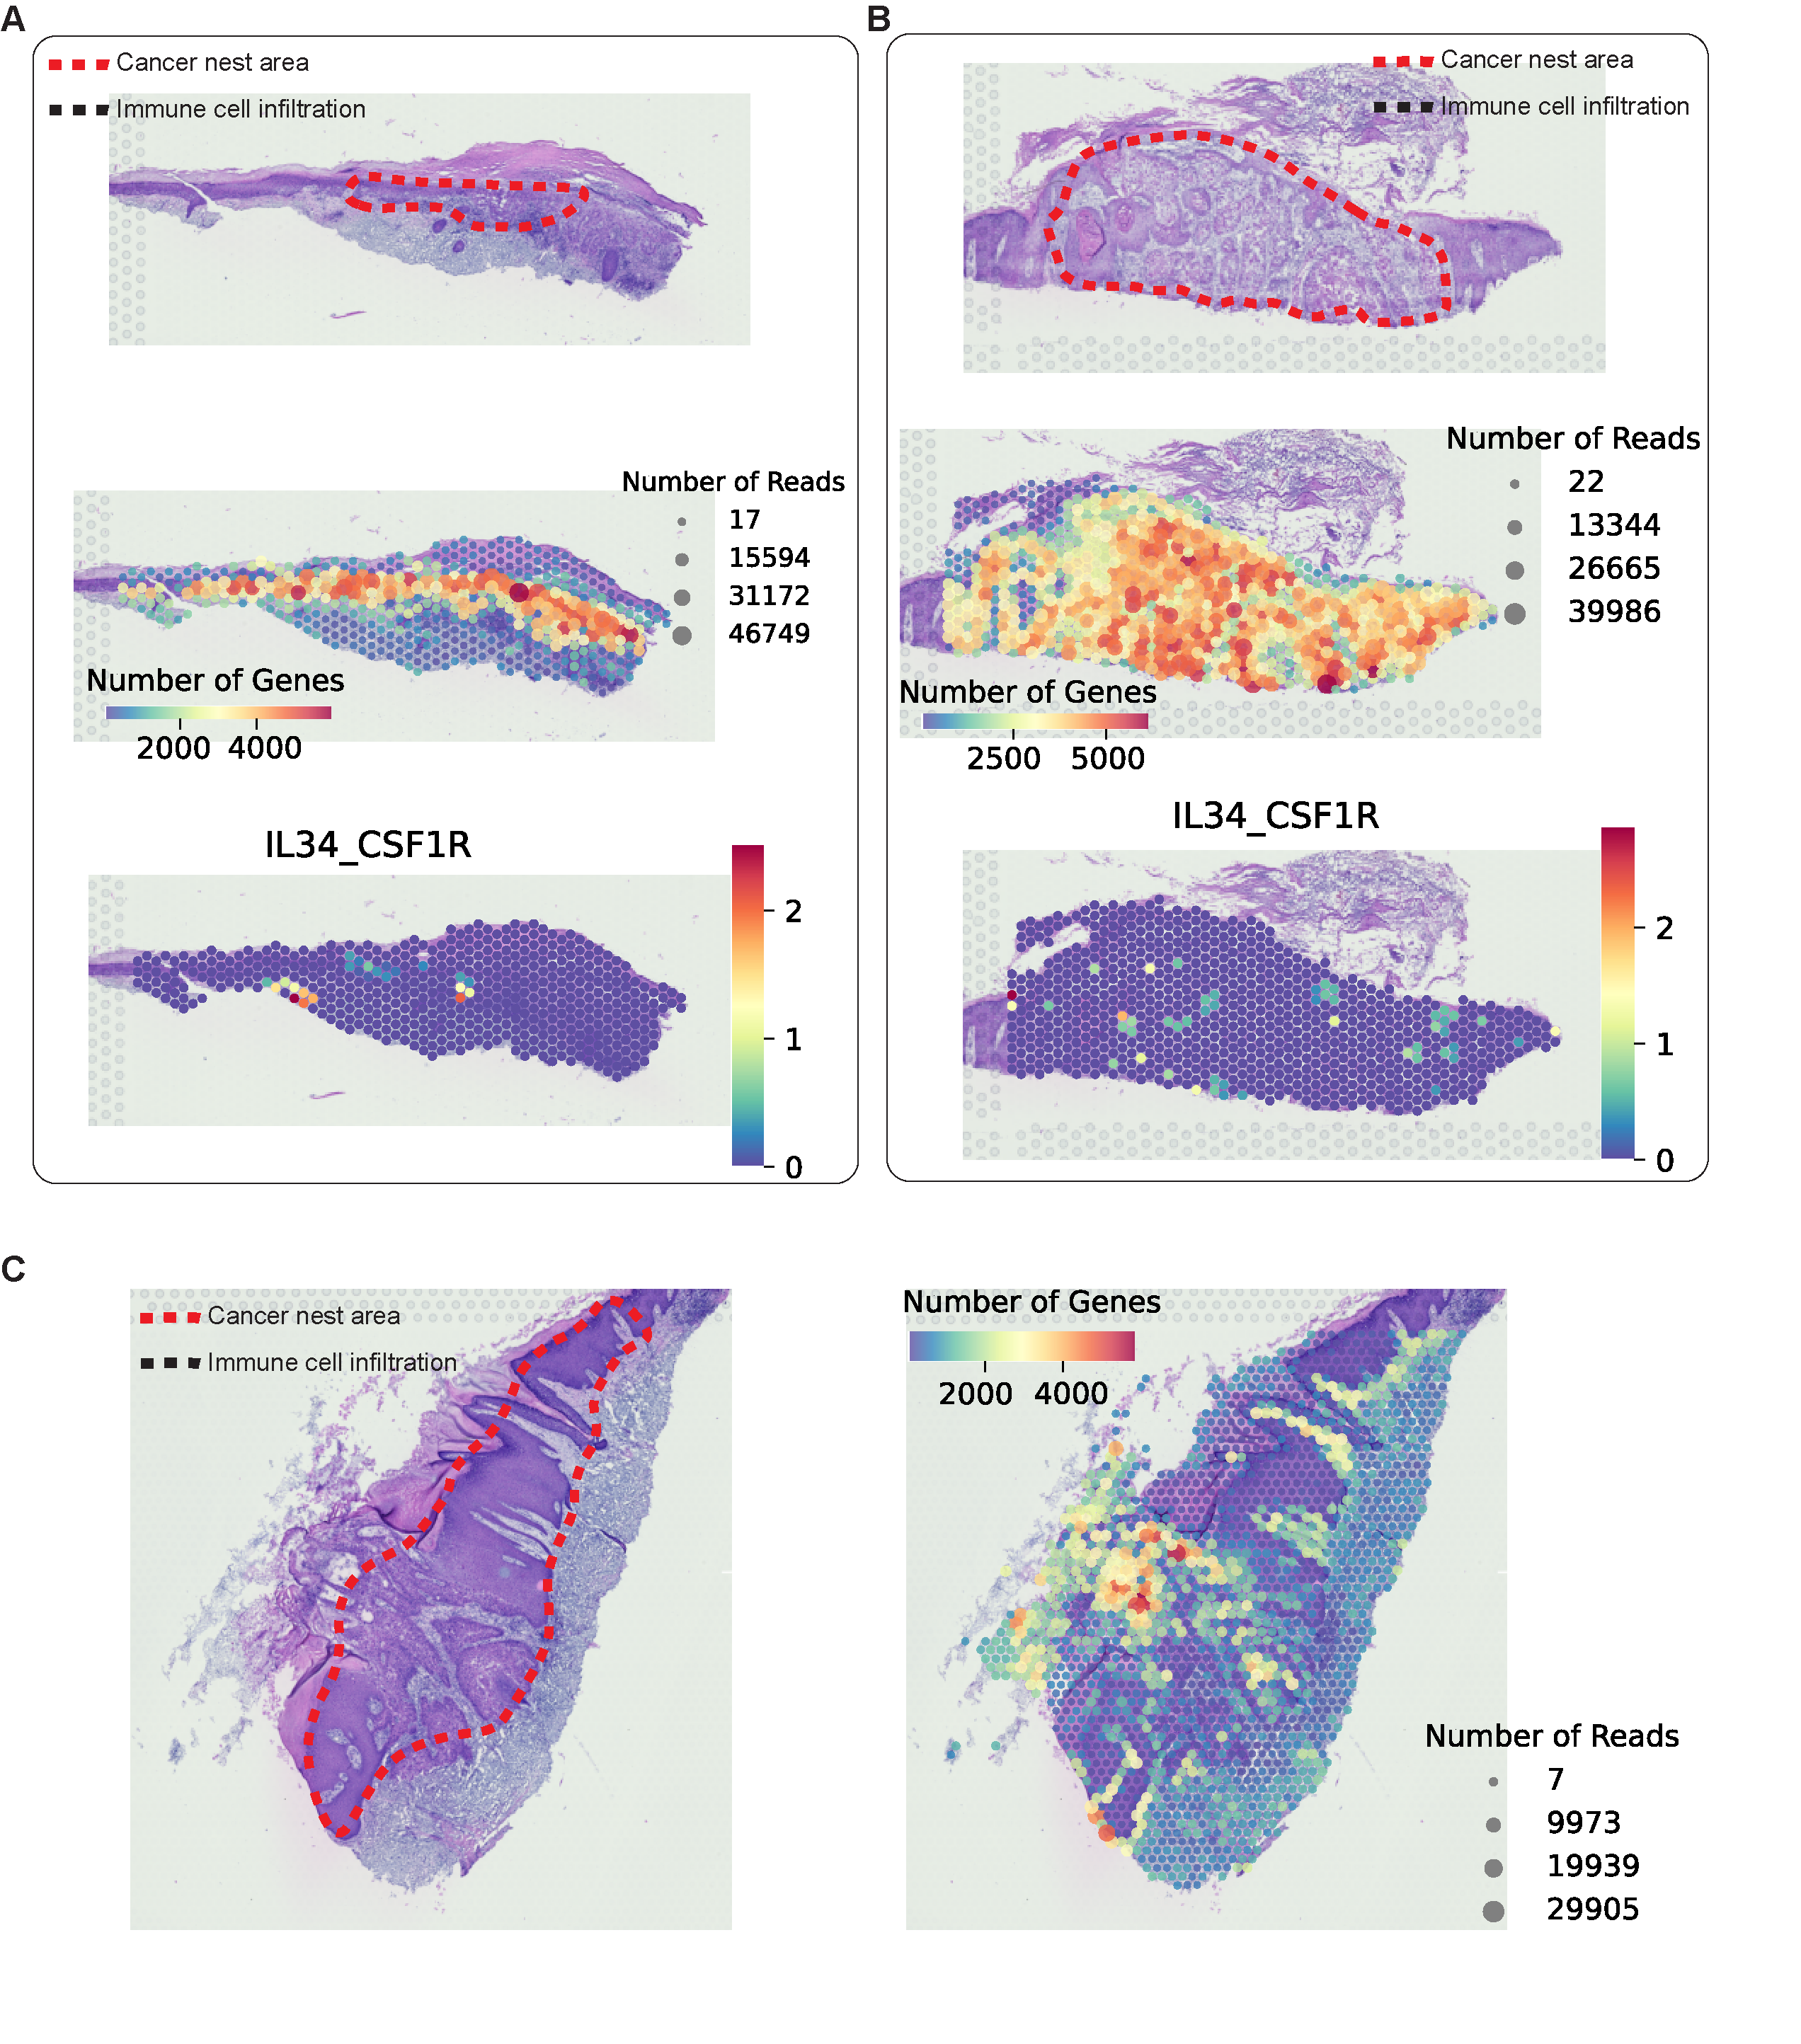
\includegraphics[width=0.75\columnwidth]{Chapter2/Figures/Supplemental_Fig_S4.png}
    \caption[Visium spatial transcriptomic for inferring cell interaction through ligand-receptor and interaction sites with spatial contexts]{Visium spatial transcriptomic for inferring cell interaction through ligand-receptor and interaction sites with spatial contexts (related to Supplemental Table 1). (A) From top to bottom, a H\&E image, the ST-seq captured and the significant spots of interaction using the pair of L-R IL34 and CSF1R (the colour bar shows the -log10 of the p-values) of BCC tissue section of patient ID-B18. (B) the H\&E image (top), the ST-seq profile of SCC patient ID-E15(middle) and the corresponding spatial distribution of significant spot with cell interaction through the pair of L-R IL34-CSF1R (bottom). (C) the H\&E image and the ST-seq captured from SCC patient ID-F21. }
    \label{fig:Chap2_Supfigure4}
\end{figure}

\subsection{Comparisons of ligand-receptor interaction between ST-seq and scRNA-seq}
% ********* Enter your text below this line: ********
We found that computational methods that did not use spatial information failed to detect expected L-R interactions. From the CellPhoneDB analysis pipeline, \cite{efremova2020cellphonedb}, a total of 1024 possible combinations of L-R were tested using the ST-seq dataset. The dot-plot in Figure \ref{fig:Chap2_figure1_result}F demonstrated the low significance of the two L-R pairs, IL34-CSF1R and THY1-amb2 complex (ITGAM pathway) in comparison to the four other CellPhoneDB highest significance of the interaction pairs. We further applied NicheNet \cite{browaeys2020nichenet} workflow on the ST-seq data to integrate prior knowledge into the prediction. While NicheNet could identify interaction pairs that were directly linked to cancer (\ie CD6-ALCAM), the prediction also failed to detect the two pairs IL34-CSF1R and THY1-ITGAM. The expression plots of the four target markers overlayed to the tissue section (Supplementary Figure \ref{fig:Chap2_Supfigure3}C, \ref{fig:Chap2_Supfigure3}D) illustrated the low abundance across the tissue, which likely suffered from the inherent dropout (randomly mis-detecting molecules due to the scRNA-seq protocol). The results suggest that for the noisy (high dropout) data and lowly-abundant genes, computational methods without spatial information like CellPhoneDB and NicheNet likely misidentify meaningful cell-cell communication (Figure \ref{fig:Chap2_figure1_result}F-G). In contrast, the addition of spatial information to test for significant local-coexpression over the background, like stLearn, could detect such signalling events (Figure \ref{fig:Chap2_figure1_result}C; Supplementary Figure \ref{fig:Chap2_Supfigure3}E,  \ref{fig:Chap2_Supfigure4}A-\ref{fig:Chap2_Supfigure4}B). Although scRNA-seq and ST-seq enable us to test for thousands of ligand-receptor pairs, their inherent technical limitations in detection sensitivity necessitate the addition of independent validation experiments that are sensitive and are not sequencing-based. Next, we describe RNAscope and our novel Spatial TRanscriptomic \textit{In Situ} Hybridization (STRISH) pipeline as a powerful experimental method for validating cell-cell interaction within spatial tissue sections. 

% ***************************************************
\subsection{STRISH framework for detecting co-localisation of cells and their ligand-receptor expression using FISH imaging}
\label{Sec:2.2_STRISH}	%CREATE YOUR OWN LABEL.

% ********* Enter your text below this line: ********
To overcome the limitations in detection sensitivity due to a lack of signal in the cancer region from the sequencing methods (scRNA-seq and ST-seq) and to achieve single-cell resolution, we implemented RNAscope HiPlex assay. RNAscope HiPlex can detect up to 12 gene targets simultaneously at single-molecule sensitivity. In this study, we used whole tissue fluorescent microscopy images captured at 40x magnification to determine RNA interaction at cellular resolution. Three different fluorophores (Cy3, Cy5 and Cy7) were used in two iterative wash-stain rounds to label the five distinct target genes, including THY1, IL34, and CSF1R, CD207 and ITGAM (Figure \ref{fig:Chap2_figure1_result}B). The zoom-in images from a cancer nest area (marked as a white dashed line, and two red/green circles - IL34 and CSF1R in a red box and THY1 and ITGAM in a green box) show distinct coexpression of neighbouring cells at single-cell resolution, suggesting cell to cell interaction for each of pair compared to no signal in the 'Negative' control. 
\begin{figure}[htp]
    \centering
    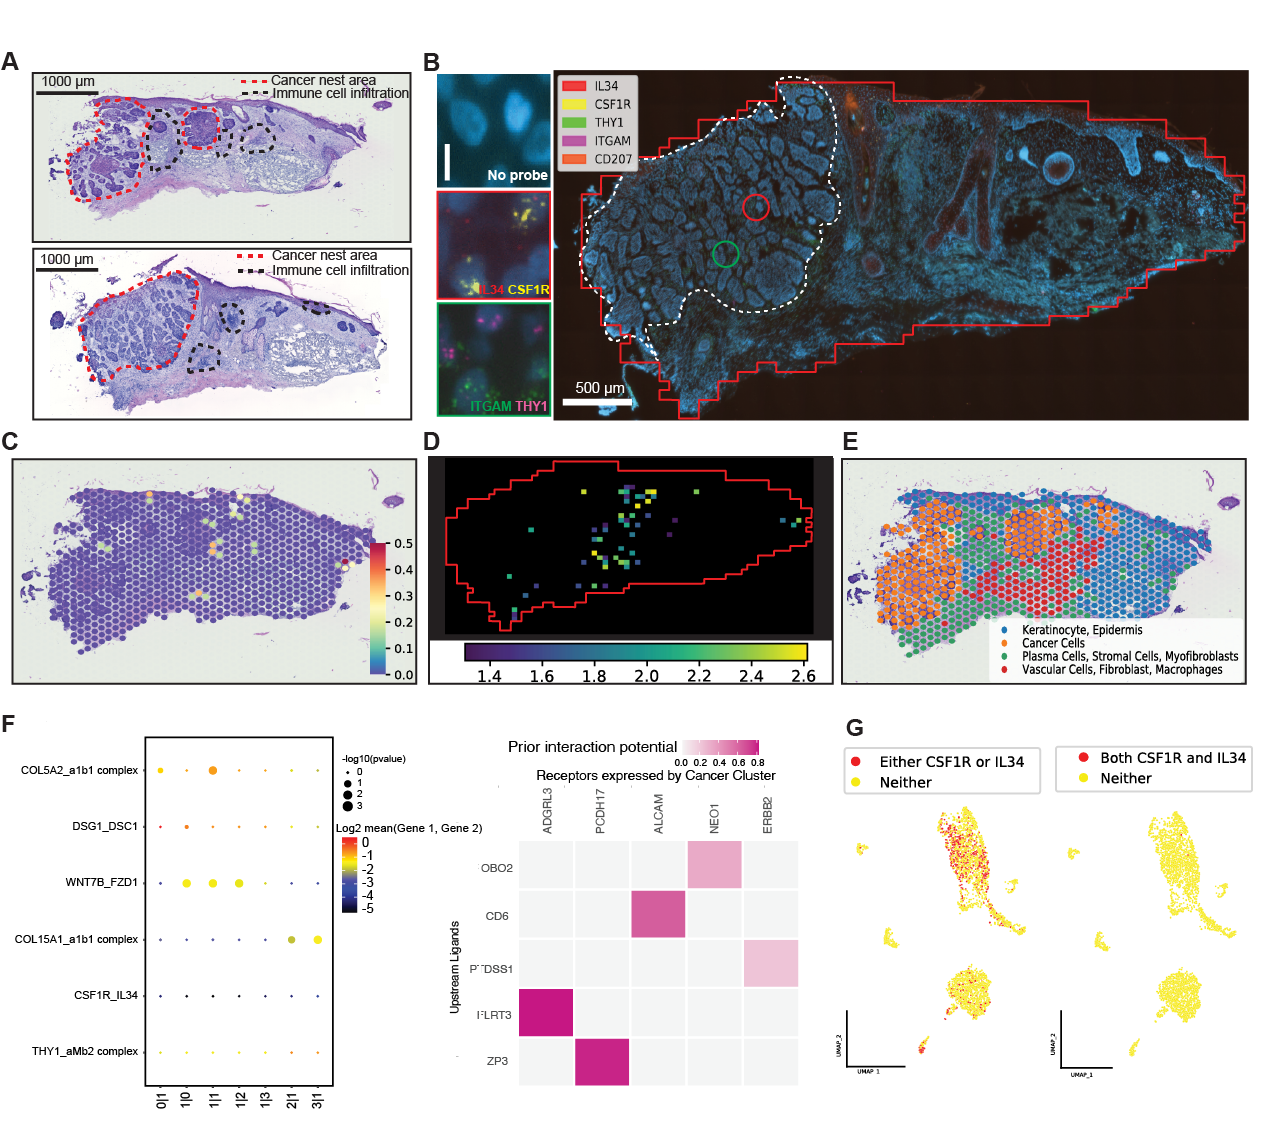
\includegraphics[width=\columnwidth]{Chapter2/Figures/Chapter2_Result_figure1.png}
    \caption[An integrated technological and computational approach to study cell-cell interaction across the whole tissue section.]{ An integrated technological and computational approach to study cell-cell interaction across the whole tissue section. (A) The annotated H\&E images of the two adjacent tissue sections that were used for Visium ST analysis (top) and the consecutive section of the same block used in RNAscope assay (bottom). (B) Target RNA molecule expression at a single cell level using RNAscope assay and the visualization of the local co-expression of two pairs L-R (C) Using ST-seq data and ligand-receptor expression analysis of neighbouring spots to determine the significant local co-expression level of IL34-CSF1R(colour bar showing the ligand-receptor score). (D) Results from our STRISH computational pipeline reported in this paper to analyse RNAscope imaging data, showing the detection of the local co-expression of IL34-CSF1R. The heatmap shows the windows with a significant level of co-expression of ligand-receptor pair (scored by -log10 of p-values). (Legend continues on the following page.)}
    \label{fig:Chap2_figure1_result}
\end{figure}
\begin{figure}[t]
  \contcaption{(E) Spatial feature plots of the four distinct clusters defined by Louvain graph-based clustering. The annotation was based on differential gene and pathway analysis. The distribution of the cluster annotated as cancer was consistent with the location of cancer nests in the upper H\&E image shown in (A). (F) The inference of L-R-based cellular communications from ST-seq data, using CellPhoneDB (left) and NicheNet (right). For CellPhoneDB prediction, the top four highly active pairs of ligand-receptor and the two target pairs were selected for visualisation. (G) The UMAP feature plots highlighted the cells that expressed either CSF1R or IL34 (red dots, left plot) and both CSF1R and IL34 (red dots, right plot)}% Continued caption
\end{figure}
STRISH pipeline consists of two phases, starting with a cell local co-expression detection step to define the spatial neighbourhood, followed by scoring, statistical testing and visualizing significant local co-expression (Figure \ref{fig:Chap2_figure2}A; Method Algorithms \ref{Chap2:Alg:01}, \ref{Chap2:Alg:02}). Local co-expression is defined as the expression within a tissue area containing fewer than a threshold number of cells (depending on tissue types), \ie fewer than 100 cells. The pipeline runs a series of positive-cell detection iterations to find regions that contain lower than the predefined threshold of neighbouring cells and subsequently determines the number of L-R co-expression within these regions (refer to the Method section about STRISH algorithm). The L-R co-expression scores are then used for a statistical test of significant coexpression over the null distribution of random, non-interacting gene-gene pairs. Across the tissue samples, we observed considerable interaction of IL34-CSF1R around the areas where the cancer nests are in both BCC and SCC, particularly in the epidermal compartments (Figure \ref{fig:Chap2_figure1_result}E, \ref{fig:Chap2_figure2}B). Interestingly, compared to RNAscope data, we observed a similar pattern in ST-seq data, with many spots that were predicted to have cell-cell communication through IL34-CSF1R located in the cancer and epidermis regions.  

We further assessed the performance of STRISH by measuring the interaction of another less abundant L-R pair, THY1-ITGAM. We found the lower signal and less widespread interaction of THY1-ITGAM that were localized to the dermal compartments (Figure \ref{fig:Chap2_figure2}B). By comparing the number of the tissue regions (through STRISH windows) where local co-expression was found, we noticed the average count of the windows with THY1 and ITGAM co-expression was, on average, 2.5 times less than those of IL34-CSF1R. Similarly, the normalized local co-expression in the same STRISH windows for ITGAM was also lower than that of IL34. We noted that most of the STRISH-detected local co-expression of THY1 and ITGAM were clustered densely around the adjacent areas of the immune cell infiltration. At the core, STRISH is constructed based on a new data structure called $STRISH\_Object$, which encapsulates the data structure from AnnData \cite{wolf2018scanpy}. Thus, STRISH is highly compatible with other single-cell platforms (\ie Scanpy \cite{wolf2018scanpy}, and Squidpy \cite{palla2022squidpy}). STRISH can also accommodate the visualization of the expression level of each marker at single-cell for quality inspection and facilitate the external validation/correlation of cell positive with markers of interest (\ie ddPCR) (Figure \ref{fig:Chap2_figure2}C). We also found that STRISH was quantitative and provided the capability of counting interaction events, an important utility that is needed in cellular communication research (Figure \ref{fig:Chap2_figure2}D; Equation \ref{chap2:eq:02}, \ref{chap2:eq:03}). Overall, we found that RNAscope data analysed by STRISH could detect cell-cell communications at a higher sensitivity than ST-seq and scRNA-seq. 

\subsection{Highly sensitive detection of ligand and receptor expression by ddPCR}
While RNAscope is expected to be able to detect single molecules in each cell, scanning through a whole tissue section with millions of cells may lead to noise and reduced accuracy due to tissue heterogeneity. ddPCR, on the other hand, enables sensitively detecting and quantifying single molecules from tissues, albeit spatial information is absent. To further confirm the presence of ligands and receptors in the tissue, we performed ddPCR on the same cancer tissue block (Figure  \ref{fig:Chap2_Supfigure6}). The transcript copy number per input RNA of each gene was presented in a bar plot (Figure \ref{fig:Chap2_Supfigure2}E). ddPCR signal was highly consistent between cells (droplets), and both L-R pairs were detected. Strikingly, the result from ddPCR was highly consistent with that of RNAscope data (Figure \ref{fig:Chap2_figure2}D, \ref{fig:Chap2_figure2}E), with Pearson correlations at 0.95, 0.89 and 0.94 for the patient samples tested, ID-E15, B18 and D04, respectively. The ddPCR results support the quantitativeness of using RNAscope for measuring target gene expression, suggesting the suitability of using RNAscope for detecting and quantifying cell-cell interaction. 

\begin{figure}[htp]
\renewcommand{\figurename}{Figure}
    \centering
    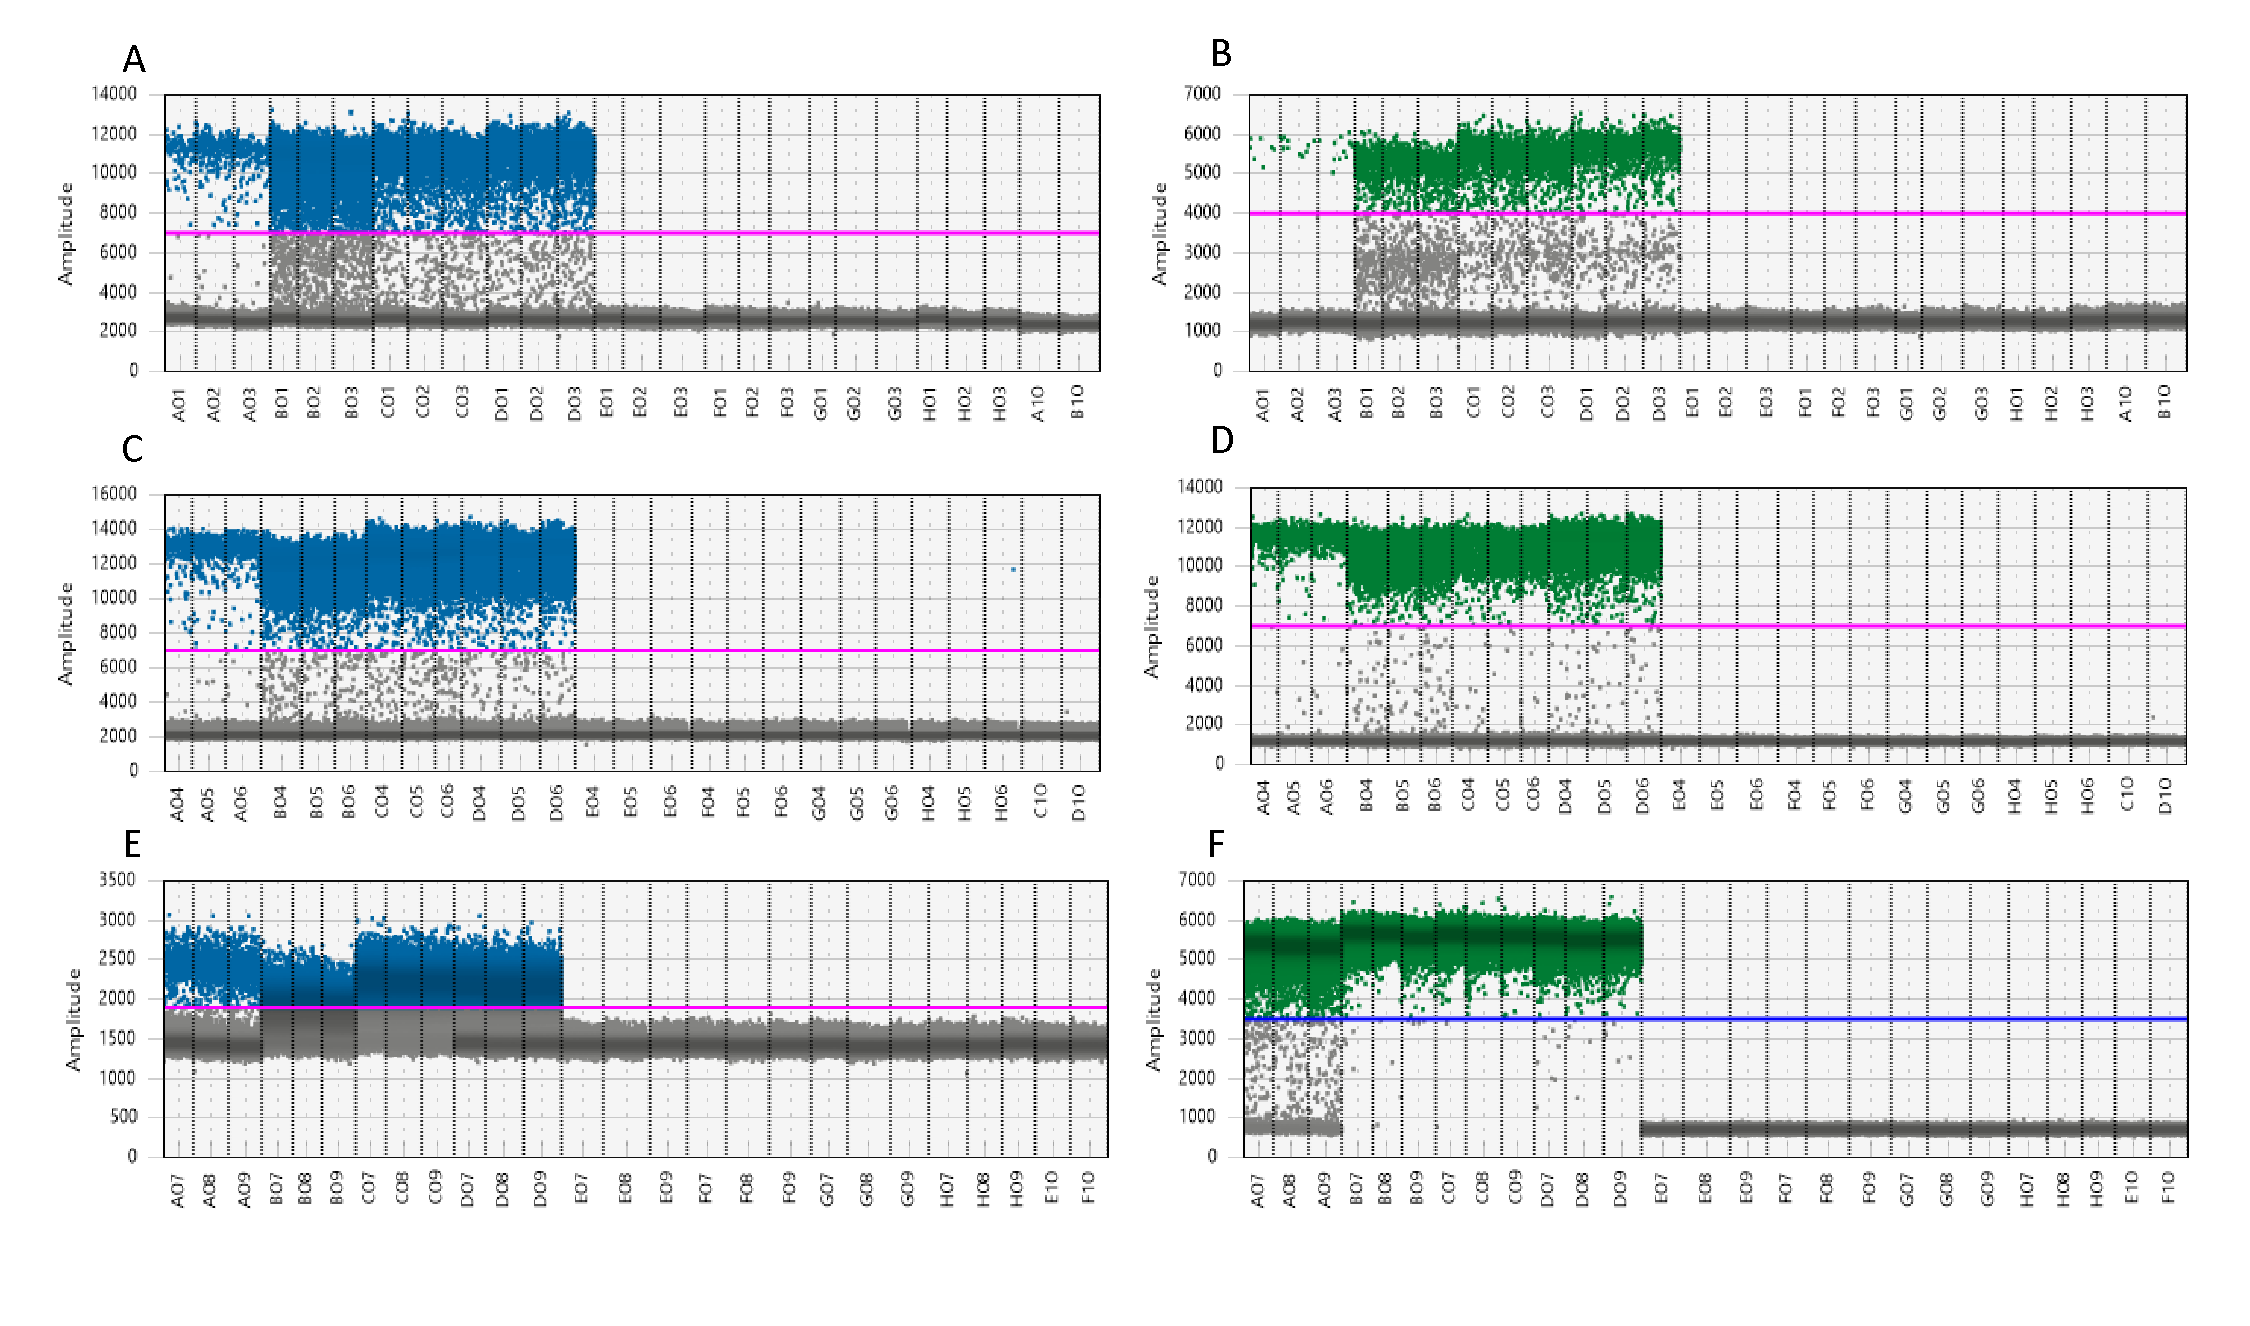
\includegraphics[width=0.75\columnwidth]{Chapter2/Figures/Supplemental_Fig_S6.png}
    \caption[Analysis of target genes by automated droplet digital PCR.]{Analysis of target genes by automated droplet digital PCR. Expression plots for data from the three BCC patients and negative controls are shown. Each blue or green point represents a single droplet. The negative droplets scored as grey if the fluorescent amplitude is lower than the detection threshold. The solid pink line indicates the threshold. FAM and HEX are reporter fluorophores conjugated to ddPCR primers to amplify templates that were later read by the QX200 droplet reader. Each gene in each droplet was read based on the labelled primer, specific to the gene.}
    \label{fig:Chap2_Supfigure6}
\end{figure}


% ***************************************************

\section{Discussion}
We presented a technological and computational end-to-end pipeline from discovery to validation of L-R interaction across the whole spatial landscape of a tumour tissue section using 4 complementary technologies. Multimodal data from these four methods allowed us to systematically examine over 1000 L-R pairs in scRNA-seq and ST-seq data, followed by deep analyses of three L-R pairs for patients with two types of non-melanoma skin cancers (BCC and SCC), which account for about 70\% of all cancer cases \cite{garcovich2017skin}. The pipeline allows us to quantitatively and visually assess the expression of target transcripts while maintaining the physiological spatial information in undissociated tissue sections. Computationally, we developed and demonstrated the utility of an imaging analysis pipeline called STRISH to automatically and statistically detect tissue regions with high cell-to-cell interaction activities, from high multiplex RNAscope RNA and Opal protein imaging data. STRISH imaging analysis results are important orthogonal validation of the predictive results from scRNA-seq and ST-seq analysis.  

For quantitative cell-cell interaction analysis, STRISH automatically scans for local co-expression of a pair of L-R genes or proteins in an RNAscope image or Opal Polaris image to recapitulate an interaction landscape across the whole tissue section. The pipeline also consists of a robust image registration step to merge two separate images from two imaging rounds, with potential application to also merge histopathological images in adjacent tissue sections. This utility allows for data integration, not only increasing the multiplex capacity to detect more L-R in one tissue section, but also adding the pathological annotation to interpret the molecular analyses. Existing image analysis tools have been developed to search for colocalization of two gene/protein markers within each individual cell \cite{bolte2006guided}. STRISH, in contrast, finds co-expression between neighbouring cells rather than within one cell, thereby identifying potential paracrine interaction between cells that are in proximity to each other. Significant regions can then be visualized in a heatmap covering the whole tissue landscape. Overall, STRISH is generalisable from assessing interactions at RNA levels like IL34-CSF1R and THY1-ITGAM in RNA-ISH multiplex assay to protein level like PD1-PD-L1 in Opal Polaris protein assay. 

Our detection of CSF1R and CSF1/IL34 interaction between cancer and immune infiltrating cells at the epidermal layers was consistent with the biological context of skin cancer. The signalling interaction between CSF1R and CSF1/IL34 is well known to regulate macrophage differentiation \cite{lin2008discovery}. IL34, CSF1 and their receptors co-expressed within the immune cell infiltrated area and regulated the different downstream signalling pathways in breast cancer \cite{zins2018differential}. CSF1R is known to be expressed on CD1a/CD207 Langerhans cells in the human epidermis and stratified epithelial \cite{lonardi2020csf1r}, where it can be found in high abundance in the basal and squamous layers of the epidermis, and is involved in anti-tumoral immune responses \cite{pogorzelska2020density}. Here, we specifically observed that the co-expression of IL34-CSF1R L-R pair is high in/near the cancer nest area in all the patient samples analysed and that the interaction was heterogeneous in high or low activities across the whole tissue section. The results are important in pinpointing the microenvironment within the tissue that can potentially be markers for cancer progression.

Our results suggest RNAscope Hiplex assay is quantitative, sensitive and high-resolution in detecting L-R interactions. RNAscope detection is more suitable than IHC in precancerous dysplastic nodules, helping early monitoring and diagnosis for patients with a high risk of diseases \cite{bakheet2020improving}. Additionally, our results from the absolute quantification of the target genes from ddPCR analysis (using adjacent tissue sections of the same tissue blocks) suggest that the RNAscope can accurately measure the expression of L-R pairs. Moreover, RNAscope can map the interactions across different locations within the tissue. This observation is important because RNAscope assay quantifies from a microscopic image that captures the fluorescent transcripts, which are usually semi-quantitative. The high correlation to ddPCR results suggests the high accuracy of the RNAscope assay. 

Here, we presented a complete pipeline from bench work to bioinformatic analysis to study cell interaction through L-R pairs in cancer tissues. We suggest using spatial transcriptomics (with whole-genome scale and with spatial information, like the Visium), followed by a targeted validation approach that is more sensitive and at a high resolution like the RNAscope and/or with an additional validation at the protein level like by using mIHC (\ie Polaris). The workflow demonstrates the feasibility of discovering new L-R pairs by genome-wide approaches (scRNA-seq and/or ST-seq), which are less sensitive but cover all genes, followed by targeted validation by high-resolution, high-multiplex, and sensitive RNAscope imaging and Opal protein imaging. The results and analyses presented in this chapter have addressed the thesis's first aim, which is to develop a novel computational analysis to locate the cell-cell interaction through L-R pair in spatial transcriptomic data.  The analytical platform that allows for the discovery and detailed analyses of more than one pair of L-R interactions in cancer tissues provides a powerful approach to finding new targets and/or understanding the mechanisms underlying options for combinatorial immunotherapies. 

So far, the analysis result presented in this chapter suggests the approach to screen for the potential L-R pair using complementary spatial transcriptomic approaches.  However, cancer is known for its heterogeneity and tumours can separate the tissue into multiple compartments. Knowledge of the spatial distribution of cells and proteins within the tissue is essential for the complete understanding of cell biology. Besides, not all transcripts will translate into proteins and the availability of technologies for spatial proteomic is also more accessible. Therefore, Chapter 3 will demonstrate a series of spatial analyses to study the cancer microenvironment and the structure of cell organisation in cancer tissues.  Particularly, Chapter 3 will discuss the analysis results conducted by spatial proteomic data to identify the spatial distribution of cell community and the heterogeneity of cell phenotype across the samples. 


% \section{Appendix}




\typeout{}

% \bibliographystyle{elsarticle-num}

% \bibliography{./References/Bibliography}
\chapter[Spatial proteomic for mapping spatial cell types and identifying interactions across tissue]{Spatial proteomic for mapping spatial cell types and identifying interactions across tissue}
\label{Chap:3}	%CREATE YOUR OWN LABEL.
\pagestyle{headings}
\section{Introduction}
\label{Sec:3.1_intro}
%CREATE YOUR OWN LABEL.
While the number of gene markers can be profiled using cutting edge spatial transcriptomic is growing rapidly, i.e. Visium (10X Genomic),  Stereo-Seq (BGI), it is important to note that not all RNA expression are highly correlated with translated protein expression level. Therefore, spatial proteomic is an important complementary tools to uncover the complex heterogeneity of cancerous cell and their intercellullar connection with other cells. Advances in multiplexed tissue imaging enables analysis of up to hundreds of proteins in thousands of cells in a single experiments. Protein profile of a tissue has been analysed, it cam provide an additional layer of connection from cells to environment context and biological processes. 

For this chapter, I focused more on quantifying the cellular structures and the cross-talk between cell types in cancer tissues using two spatial proteomics technologies: Vectra Polaris in skin cancer and Imaging Mass Cytometry (IMC) \cite{giesen2014IMC} in colorectal cancer (Table: \ref{table:DataInfor}). The former dataset I was working on  consists of 6 whole slide skin cancer tissues which were scanned by highly multiplex Polaris technologies. Each slide was processed with a panel of 6 proteins CD8, PD-L1, PD-1, FoxP3, CD68, Pan-cytokeratin (PanCK) and DAPI for nuclei staining. Meanwhile for the colorectal cancer, the experiment was designed to use IMC technology to capture the protein expression of a panel of 15 protein markers from 51 patients with stage 3 colon adenocarcinoma. The IMC protein panel consists of structural markers  Epithelial (E-cadherin, Keratin), Fibroblast (collagen), cell proliferative marker (Ki-67) and several immune markers including for T-cells (CD8), regulatory T cells (FoxP3), macrophages (CD68+), B cells (CD20+), etc. Unlike Polaris technology, IMC performs tissue scanning at multiple regions of interest (ROIs) selected from whole slide tissue. Although, the two input datasets captured different antibody panels as well as different cancer types, they both produce protein expression data at subcellular resolution retaining  a wealth of spatial information.    

\begin{table}[ht]
\centering
\caption{Summary of data specification}
\begin{tabular}{||P{7cm} || P{3cm} || P{3cm} ||} 
 \hline
 Specifications & Colorectal Cancer Samples & Skin Cancer Samples   \\ [0.33ex] 
 \hline\hline
 Number of patients & 52 & 3   \\ 
 \hline
 Number of Markers & 16 markers & 6 markers  \\ 
 \hline
 Number of images & 126 ROIs &  6 whole slides \\
 \hline
 Diagnosis & Stage 3 adenocarcinoma & Basal Cell Carcinoma  \\ [1ex] 
 \hline
\end{tabular}
\label{table:DataInfor}
\end{table}


% ***************************************************
\section{Cell type identification and cell communities detection methods}
\label{Sec:3.2_CCC_ST}	%CREATE YOUR OWN LABEL.
\subsection{Adapting cell type identification from existing scRNA-seq methods}
Before any CCC analysis, a key step  to make use of sub-cellular spatial proteomic information is to perform cell segmentation and cell type identification. Depending on the size of the whole slide tissue, Polaris imaging in our skin cancer dataset captured around $40000\sim 79000$ cells per tissue with fluorescence values quantified for each marker. To employ the current established cell clustering and annotation, the Polaris imaging was transformed into a non-imaging-based data through cell segmentation (Figure: \ref{fig:Polaris_skin_cancer_cell_iden}A,B) \cite{hickey2021strategies}. More specifically, cell segmentation was carried out throughout the tissue using a deep learning model called stardist \cite{schmidt2018cell}, which eventually turned every nuclei in the DAPI channel into a list of cell objects. For each cell object, the protein signal intensity was normalised to the mean DAPI intensity within cell boundary and assigned to expression level of that protein to the cell (Figure: \ref{fig:Polaris_skin_cancer_cell_iden}B-D). In order to remove the artificially high background from fluorescent intensities (outliers), $95^{th}$ percentile was used to cap the maximum value of each marker (Figure: \ref{fig:Polaris_skin_cancer_cell_iden}D). After the preprocessing of proteomics data, a standard cell type clustering was applied using a common single-cell processing pipeline, scanpy \cite{wolf2018scanpy}. Based on the panel of 6 proteins, we were able to identify several major epithelial (PanCK+), inmate immune cells (CD68+) and adaptive immune cells (CD8+, FoxP3+) (Fig: \ref{fig:skin_cancer_polaris}A). Among all the clusters detected by the scanpy pipeline (leiden clustering), those cells with very low expression of all the proteins in the panel were classified as unidentified and removed from downstream analysis. The cell identifications were eventually plotted back to the original spatial context for validation.  

Similarly, for our IMC imaging dataset of colorectal cancer, the first analysis steps are cell segmentation and cell clustering. The key differences between Polaris and IMC are the resolution of the images generated by each technology. While every pixel in the Polaris image captures $0.49 \mu m$ in the real tissue, the specification in IMC is $1$pixel representing $1\mu m$. IMC generated discrete signal (counts of heavy metal molecules) which requires a specialised cell segmentation method. Currently, the IMC segmentation pipeline is being adapted from a pipeline by Bodenmiller Group, one of the founders of the technology (\href{https://github.com/BodenmillerGroup/ImcSegmentationPipeline/blob/development/scripts/imc_preprocessing.ipynb}{Github IMC preprocessing pipeline}. In short, the raw IMC data (.mcd file) are converted into a standard image format with multiple channels and each channel represent the expression of a staining marker. Because the signal intensity in IMC has lower resolution yet noisier than in Polaris, we manually built a segmentation model to assign pixels to either cell nuclei, cytoplasm or background using two steps with CellProfiler and Ilastik \cite{carpenter2006cellprofiler, berg2019ilastik}. Since IMC imaging data were generated only for selected ROI, not the whole tissue, the number of cells in this project is significantly lower than that in the skin cancer project, ranging from $200$ to $1600$ cells per ROI (~3 ROIs/sample) . After the cell segmentation, similar data preprocessing is applied to map signals to a list of cell objects. Cellular data was then clipped to remove outliers. For cell type annotation, major structural cell types could be identified with high confidence such as Epithelial or Cancer (E-cadherin and Keratin), Fibroblast and Stromal (Collagen, SM-actin). We were also able to annotate other adaptive like B-cells (CD20), CD8 T-cells (CD8), T-reg cells (CD4, FoxP3) and inmate immune cell type Macrophages (CD68) (Fig:\ref{fig:colorectal_cancer_IMC}A). Finally, for validation, we compared the IMC-identified cell types against pathologist annotation. Through a process called image registration, we were able to align the IMC image to the adjacent section of H\&E image which was annotated with some cell types by pathologist (Fig:\ref{fig:colorectal_cancer_IMC}B). Since our computational results matched well with manual annotation this gave us confidence in our cell segmentation and clustering approaches before proceeding towards the CCC analyses. 

\begin{figure}[htp]
    \centering
    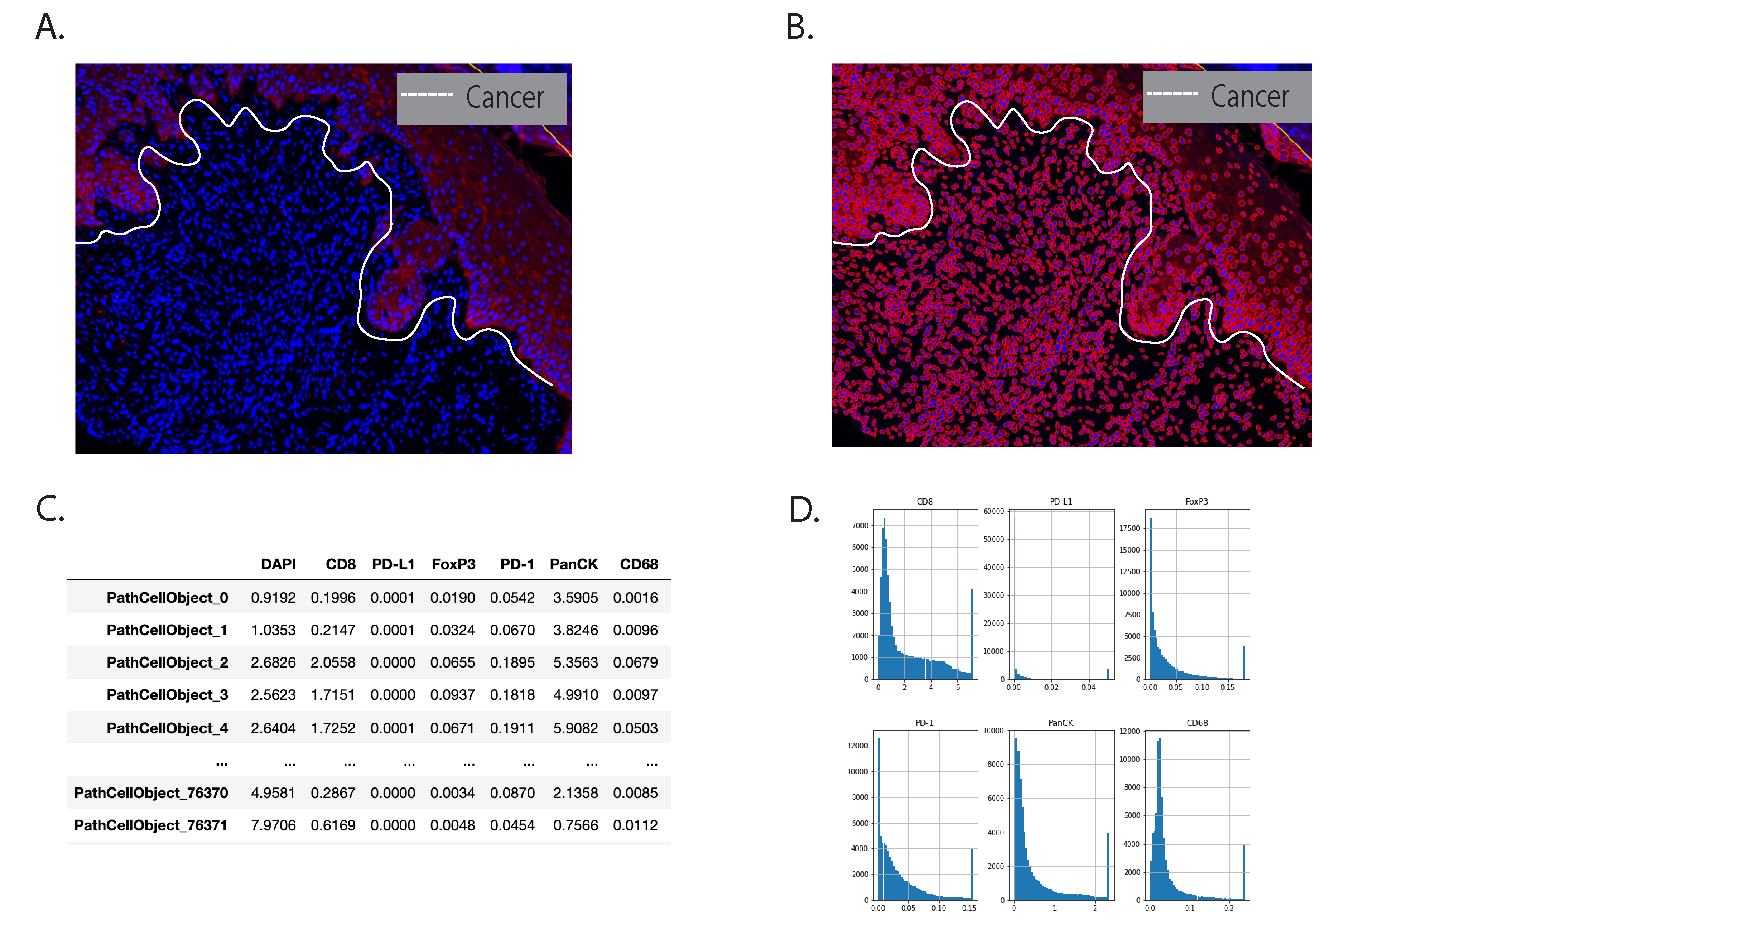
\includegraphics[width=\columnwidth]{Chapter3/Figures/Cell_identification_skin_cancer-01.png}
    \caption{Schematic of data preprocessing for cell type annotation. (A) A zoomed in image of cell the nuclei representation in DAPI channel (dark blue) and cytokeratin marker expression (PanCK in red) for epithelial cell marker. The annotation line in white separates the cancer lesions of the skin from the lower layer. (B) Detection and segmentation of cells from the image using the nuclei channel. (C) The conversion of imaging-based data to single-cell-based data by measuring the level signal each cell expresses within the cell boundary. (D) Histograms of the expression level of each protein in the panels across all the detection cells}
    \label{fig:Polaris_skin_cancer_cell_iden}
\end{figure}

\subsection{Detecting cell communities based on cells spatial organisation}
There are already a few computational methods that used scRNA-seq to infer the CCC i.e. CellChat \cite{jin2021CellChat}, CellPhoneDB \cite{efremova2020cellphonedb} or NicheNet \cite{browaeys2020nichenet}. However, they are all unable to address the spatial constraints of interactions. With scRNA-seq data, the limited insights into the spatial location of the RNA molecules within a cell and the organization of cells in a tissue prevent the CCC inference from reaching its potential. To address this, the development of higher multiplexed histological techniques for capturing transcriptomic or/and proteomic information at subcellular resolution, e.g. co-detection by imaging (CODEX) \cite{goltsev2018CODEX} or IMC from Hyperion, facilitated the integration of spatial information into CCC inference. 

Given the growing number of spatially resolved transcriptomic and proteomic technologies, the current available analysis strategies to process these high dimensional data have not yet exploited the full potential of spatial information. In short, spatially resolved CCC analysis can be categorised into two main groups. The first approach considers each cell as a point in Cartesian coordinate system and assesses the changes in the spatial co-localisation between pairs of cell types at distances \cite{arnol2019modeling,schurch2020coordinated}. Meanwhile, the second path considers only the interactions of each cell and its intermediate adjacent cells within a short proximity from the cell membrane. It is sufficient to measure cell-cell interaction through gap junction or paracrine signalling. The pairwise interaction of two cell types is then grouped by cell phenotypes and compared to randomised label of cells to determine significance of interactions  \cite{schapiro2017histocat}.  In the following sections, I will go deeper into the advantages and disadvantages of each approach and about how I applied them throughout my second-year projects.    

PD1 has been extensively studied and identified as immune inhibitor for skin cancer cell growth\cite{ishida1992induced,  tsai2014pd}. In the first project using skin cancer as the model to study, we were interested in finding and validating the immune-cancer cell interactions pairing the ligand-receptor PD-L1 and PD1 through a series of spatial analysis methods. On the other hand, we sought to find the pattern of intercellular architecture in colorectal cancer and the correlation between alterations in CCC and the prognosis for the patients. Once the cells were clustered and annotated appropriately, we to applied multiple spatial analyses to study cell-cell interactions with the aim of improving the capability to predict the clinical outcome. For each project, we performed two to three neighbourhood analyses to explore and quantify the tissue section finds.  

\begin{figure}
    \centering
    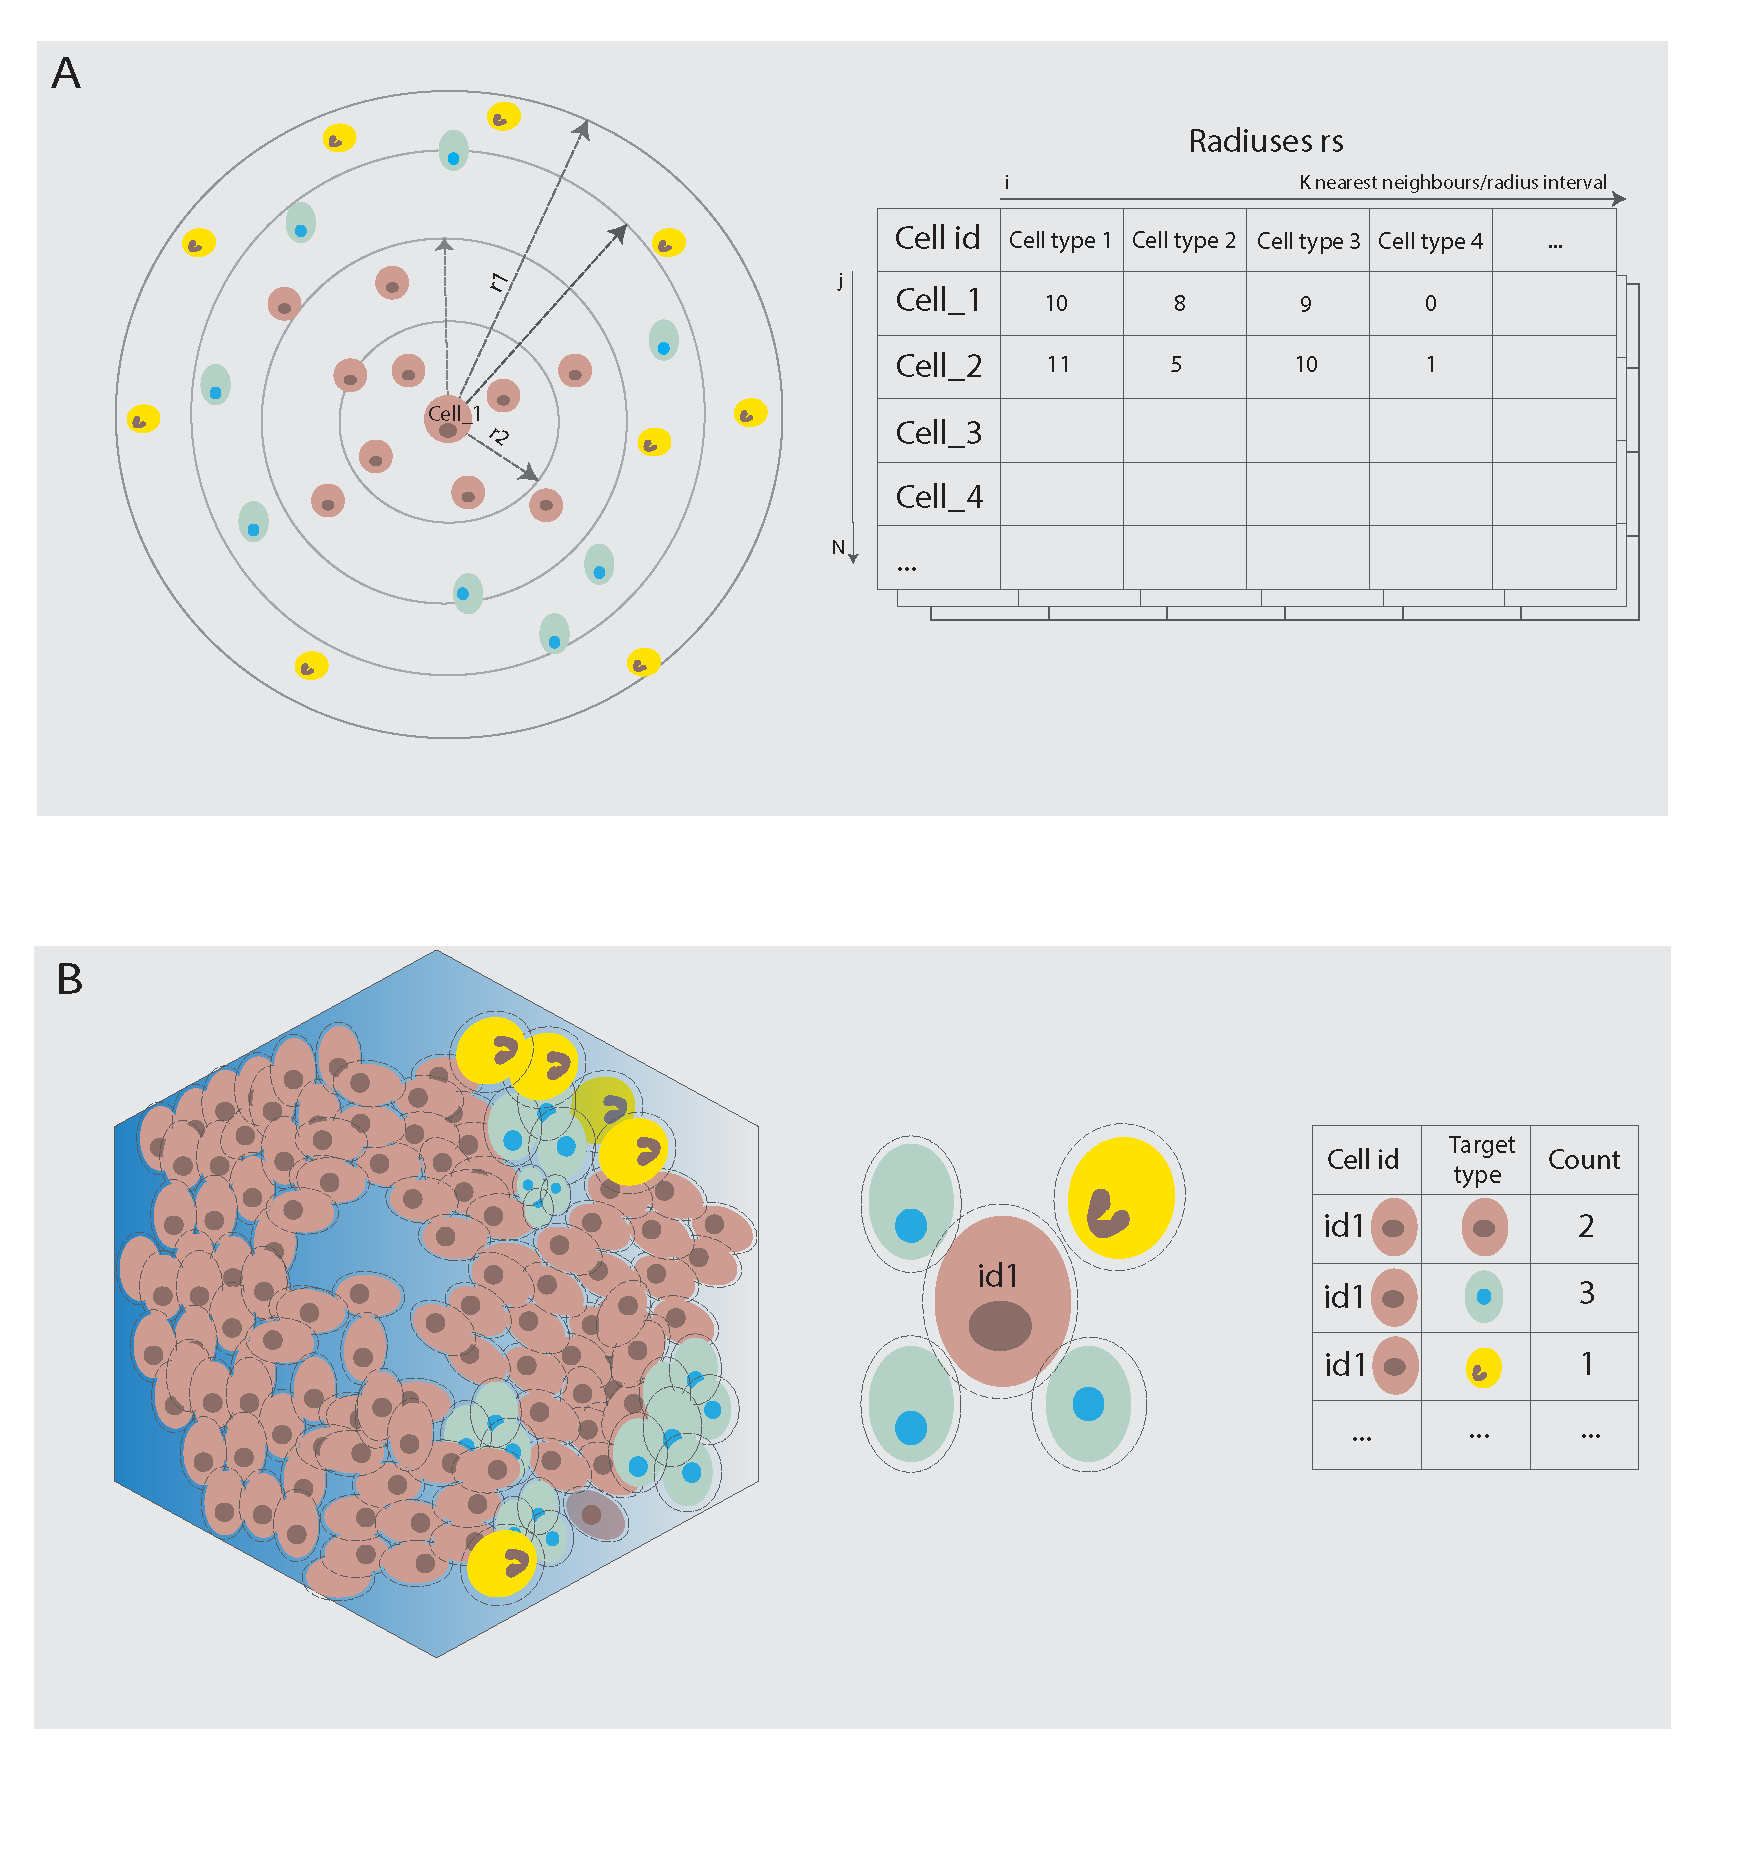
\includegraphics[width=0.85\columnwidth]{Chapter3/Figures/Conceptualise_CCC_analysis_cropped-01.png}
    \caption{Summary of different cell type interaction analyses. (A) Schematic of cell-cell interaction through varied distance interval. The analysis process starts by iterating through every cell then accumulates the information about neighbouring cells to determine the cell spatial identity. (B) Schematic of measuring spatial interaction of cells through counting the number of touching cells. Randomising is applied at the downstream of the analysis to identify the significance of pairwise interaction}
    \label{fig:CCC_conceptualised}
\end{figure}

\subsection{Nearest neighbourhood approach to cells interaction}
% ********* Enter your text below this line: ********
For the second aims of this thesis, I implemented and adopted several methods to uncover the tissue spatial organization by considering each cell as a point process in a 2-dimensional coordinate system. The advantage of this point-process approach is that it can use most of the analytical procedure established in high-level spatial analyses in social studies \cite{yushimito2012voronoi}. It is reasoned that the spatial structure of the tissue is a heterogeneous collection of single cells, consisting of multiple homogeneous groups \cite{schurch2020coordinated}. In this approach, we identify spatial communities throughout the tissue using $K$ nearest neighbour and/or a radial distance approach (Fig: \ref{fig:CCC_conceptualised}A). For each cell across the tissue, the spatial identity of itself is defined by a K number of nearest neighbouring cells (including itself as the reference). The nearest neighbour metric is measured by Euclidean distance between the $X$ and $Y$ coordinates of the cells in the two dimensional tissue section. Alternatively, we can also apply a neighbourhood identification method that is threshold free, known as the Delaunay cell network \cite{guibas1985primitives, dries2021giotto}. The spatial identities of cells are then clustered by their neighbourhood features \ref{fig:CCC_conceptualised}. The clusters of cells based on cell neighbourhood (i.e. spatial identity) can reveal communities of cells within the tissue and the composition of cell type for each community. Such methods have been used and adopted in different fields including eco-geography as well as biology \cite{goltsev2018CODEX, dries2021giotto}.

To ascertain whether cell communities identified by the above approaches followed true spatial patterns, we performed co-occurrence analysis which also employs similar principles as in the nearest neighbourhood approach. This co-occurrence analysis was inspired by an approach introduced by Tosti et al., first applied for spatial transcriptomics data of human pancreas \cite{tosti2021single}. The co-occurrence score can be estimated by the Equation \ref{Eq:Cooc_equation}, which is defined by the fraction of the probability of observing a test cell type $exp$ at the presence of a reference cell type $cond$ ($P_{r}(exp|cond)$) over the probability of observing that test cell type $exp$ $P_{r}(exp)$ at the presence of any other cell type within the same distant interval $r$. At a specific distant $r$, $Co_{r}$ indicates how high/low $exp$ and $cond$ cell types co-localised compared to random cell types. The comparison of $Co_{r}$ at an increasing distant radii $r$ shows how the co-localisation of two cell types starts dispersing.[...]


\begin{align}
\label{Eq:Cooc_equation}
Co_{r} = \frac{P_{r}(exp|cond)}{P_{r}(exp)} 
% K(t) =  \sum_{i=1}^{n}\sum_{n}^{j}1\{d_{ij} < r\} \\ 
\end{align}

For the Polaris skin cancer dataset, we first investigated how different cell types are colocalised into communities using the nearest neighbour approach. By clustering analysis to group regions with similar local density of various cell types, we identified 6 cell communities distributed across the tissue. Quantitative assessment of cell composition in each community allowed us to deduce biologically interpretable features of these communities (Fig: \ref{fig:skin_cancer_polaris}A). Particularly, communities 2 and 3 consisted of scattered immune cells while community 1 appeared to have very high density of epithelial cells positive with PD-L1. This could be explained by the known biological process and tissue structure that cancerous epithelial cells tend to reside densely around the cancer nest, and the presence of immune cells under the epidermis layer (Fig: \ref{fig:skin_cancer_polaris}B,E). On the other hand, clusters 1 and 4 contain mixed epithelial and immune cell populations in the same communities. Comparing the distribution of cell communities and tissue annotation (Fig: \ref{fig:skin_cancer_polaris}B) suggested that the clusters 2, 3 and 4 highly aligned with the stromal microenvironment communities (Fig: \ref{fig:skin_cancer_polaris}D).  Of note, using our own STRISH test (described in more details later), we found spatially-specific interactions between PD1 and PDL1 along the edge of cancer and immune cells \ref{fig:skin_cancer_polaris}C). Furthermore, we investigated the clusters 2 and 3 by co-occurrence analysis (Fig: \ref{fig:skin_cancer_polaris}F). Using T-cells positive with PD1+ protein as the condition (reference) cell type), the co-occurence test confirmed that the co-localisation of these cells with the other two subgroups of T-cells, including double positives CD8+ and FoxP3+ and single positive CD8+ T-cells were higher than random (at distances from $0\mu m$ to $400 \mu m$). Similarly, PanCK+ also co-occured with the CD68+ and PD1+ double positive cluster.       

Applying similar CCC analysis approaches to the colorectal dataset, we sought to test for the co-localization between cancer and immune cells across ROIs. As an example, the general distribution of cells and signals within an ROI is shown in \ref{fig:colorectal_cancer_IMC}A and \ref{fig:colorectal_cancer_IMC}B. Figure \ref{fig:colorectal_cancer_IMC}D shows the probability conditioned on the presence of cancer cells of the ROIs showed in \ref{fig:colorectal_cancer_IMC}A. We could observe a high enrichment of of cancer cells with epithelial cells at the first $200\mu m$ interval. While the co-occurrence analysis could provide insights into how different cell types form cell communities, the analysis is limited to a single ROI at a time. Therefore, we performed an additional analysis where we grouped co-occurrence scores of multiple ROIs together which allowed us to perform Wilcoxon test for the significance of co-localization. The table embedded in the Figure\ref{fig:colorectal_cancer_IMC}E shows the significant test of occurrence scores of between every pair of cell types in our dataset. This new statistical test framework is being developed, and the preliminary results suggested differential cell type co-localisation across patients and should be suitable features to be correlated with clinical outcomes.[...]

\begin{figure}
    \centering
    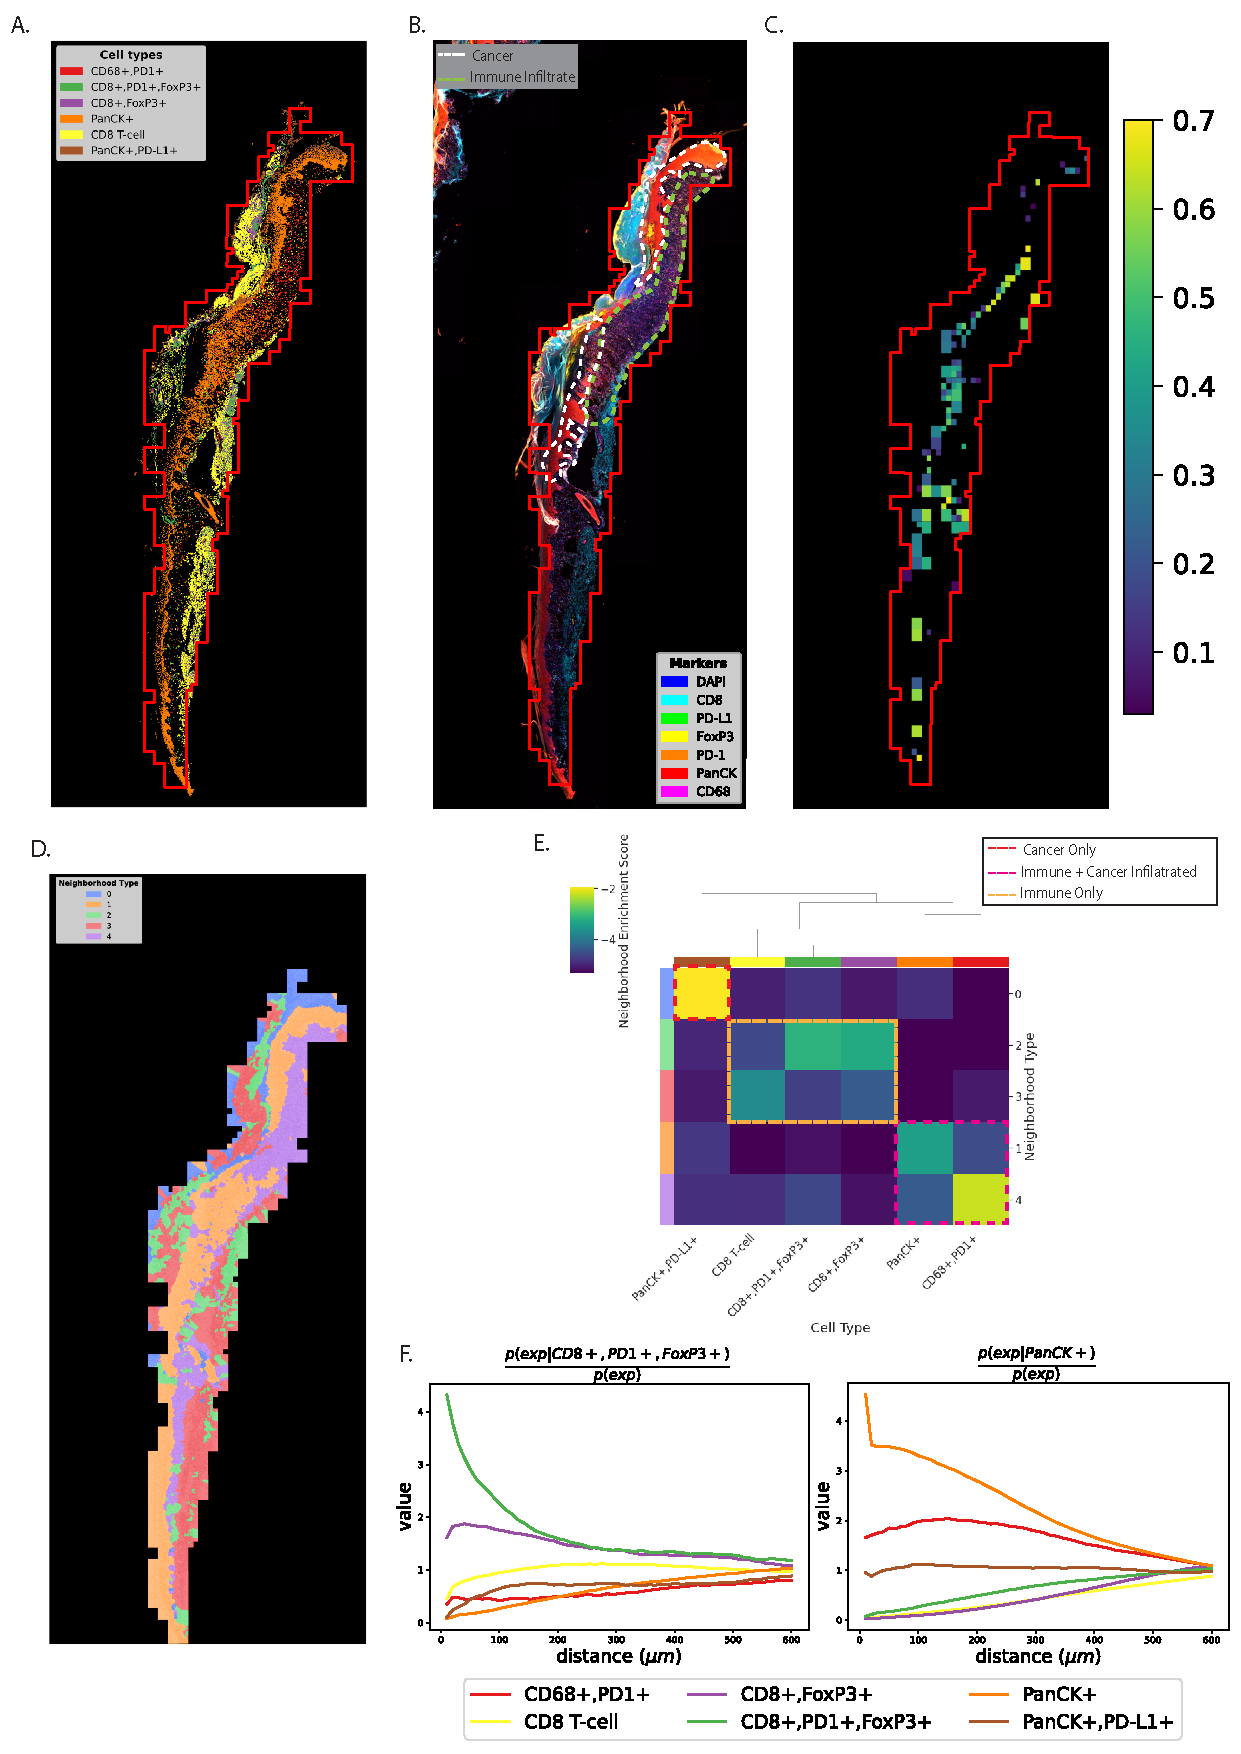
\includegraphics[width=0.8\columnwidth]{Chapter3/Figures/Minh_figure3-01.png}
    \caption{Analyses of Polaris multiplexed imaging of human SCC skin cancer tissue. (A) Cell type classification through clustering and signal gating of the expression of 6 proteins mapped to single cells. The panel of 6 antibodies used to profile the protein expression of major cell types of interest including cytokeratin, cancer secrete immune inhibitor (PD-L1), and immune cells (CD8 T-cell, NK cells, Macrophages). (B) Pathological annotation of cancer and immune regions, based on tissue morphology. (C) Analysis of cancer-immune cell co-localisation through the ligand-receptor pair PD1 and PD-L1. (D) Voronoi which uses the spatial distribution of the cell communities to split the original tissue into multiple regions, representation of distinct cell neighbourhood communities defined via clustering}
    \label{fig:skin_cancer_polaris}
    
\end{figure}
\subsection{A contact-based approach for CCC analysis}
For the colorectal cancer project, we do not have the pathologist annotations for all the ROIs. Therefore, we adopted a slightly different approach to measure near distant CCC. Using the cell segmentation masks as the representation of the cells, we expanded the peripheral of the cell by a margin of 6 pixels and counted the number of touching cells in the adjacent space for pairwise interaction analysis (Figure: \ref{fig:CCC_conceptualised}B). The pairwise interaction was compared to a random distribution using two individual one-tail permutation test within the same image. The test suggested how significant a pairwise interaction between two cell types was compared to random, and eventually suggested an interaction or an avoidance trend. The significance ($P<0.05$) of the contact-based neighbourhood analysis in one of the ROIs shows the most significant interaction starting from epithelial cells toward fibroblast cells. The next significant interactions included those of cancer cells with macrophages and with NK-cells (equally) (Fig: \ref{fig:colorectal_cancer_IMC}C). These results make biological sense and are expected as the cause of colorectal adenocarcinoma are mutated epithelial cells which trigger the growth of surrounding  stromal cells \cite{bremnes2011role}. 

A statistical test to combine the multiple ROIs and tissue sample together for survival prediction and clinical outcome using CCC is also another interesting analysis that I sought to develop and implement on those datasets. Through the multiple spatial methods of cell-cell interaction analyses that I have done so far, I look forward to combining them into a full and comprehensive pipeline for studying CCC with spatial -omic data. This next step is also aligned with my third aim to develop a holistic framework to work with multimodal spatial -omic data and discover different characteristics of CCC throughout cancer tissues. 

% histocat approach which uses the cell outline
\begin{figure}
    \centering
    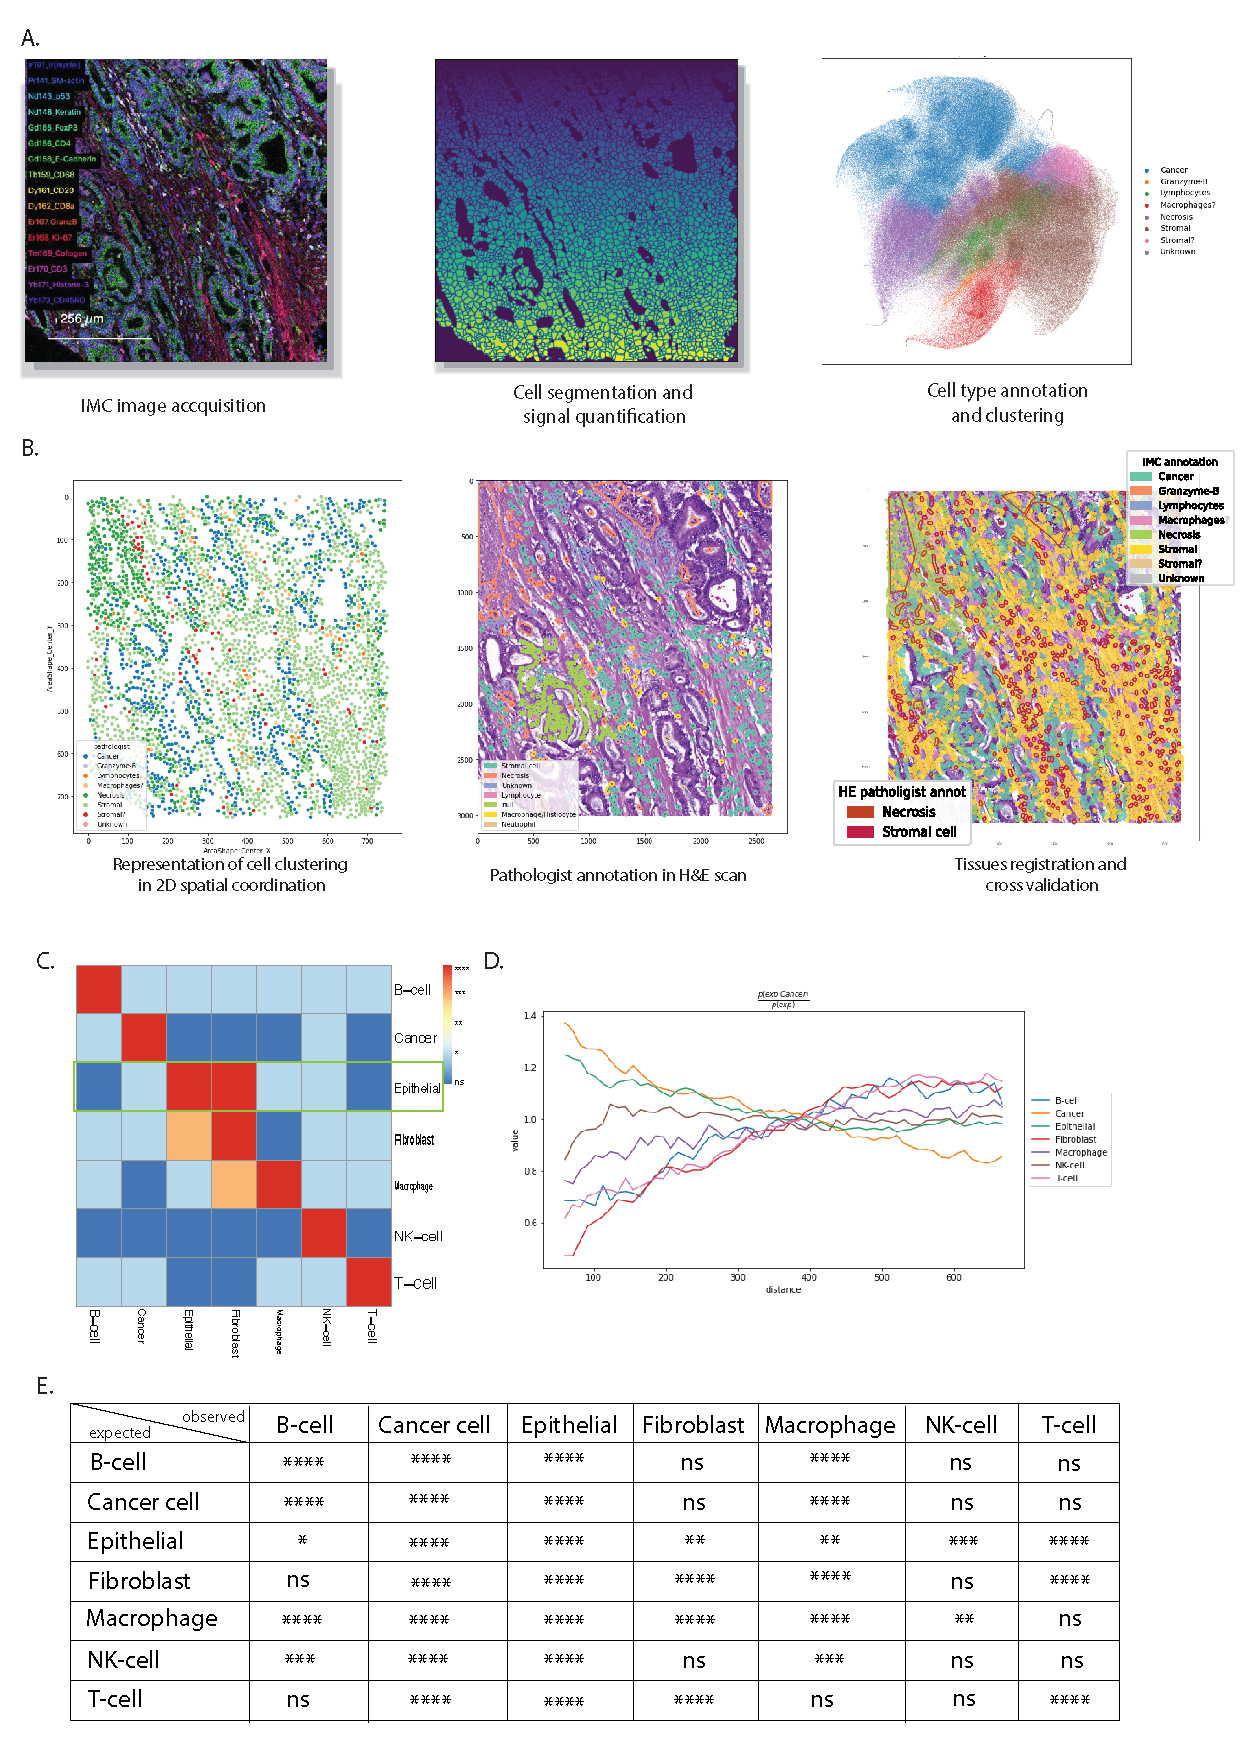
\includegraphics[width=0.8\columnwidth]{Chapter3/Figures/Hyperion_analysis_results-01.png}
    \caption{Keys analysis components of cell type identification and CCC for IMC data. (A) The workflow for the transformation from multiplexed imaging data to non-imaging, single-cell data for clustering pipeline. (B) Visualization of cell type annotation and validation against pathologist H\&E annotation. (C) The landscape of intercellular communication across a sub-sample of the whole IMC dataset. (D) An example of co-occurrence analysis of different cell types in the presence of cancer cells at increasing distance thresholds. (E) A summary of significance co-occurrence score across all combinations of observed and expected cell types.}
    \label{fig:colorectal_cancer_IMC}
    
\end{figure}
% ***************************************************
\section{STRISH for cell co-localisation with spatial proteomic data}
\label{Sec:3.3_STRISH2.0}	%CREATE YOUR OWN LABEL.
Spatial information at the subcellular level can facilitate a lower level of spatial analysis, which uses the cell geometry and density to assist the interaction analysis. As described before, in the Polaris dataset, we scanned all the regions, where cancer and immune cells co-localised and interacted via PD-L1 and PD1. Using the cell clustering information, I developed and applied a STRISH scanning window strategy to search for regions where there are immune cells double positive for CD8+ and PD1+ in the immediate vicinity of cancerous epithelial cells (which themselves are double positive for PanCK+ and PD-L1+). The STRISH scanning window strategy starts with a broad scale (i.e 4 non-overlapped tiles at the size of of one fourth of the original slide scan) and gradually splits large tiles into smaller windows until a cell-count threshold is met (less than 100 cell per windows by default). Subsequently, the results from cell detection are scored, normalised and used to plot a heatmap for localised regions (neighbourhood) with co-localisation of the two cell types being tested. Figure \ref{fig:skin_cancer_polaris}C shows the activity map of CD8+, PD1+ cells and PanCK+, PD-L1+ cells throughout the tissue. Interestingly, these two cell types were mostly observed to be co-localised at the interface of cancer and immune infiltration, according to the pathologist's annotation. The heatmap provided visual and quantitative evidence of CCC occurring between cells in our tissue sample. This analysis result is being integrated in a multimodal project to create atlas of skin cancer and cell-cell interaction with other 5 complementary technologies (manuscript under preparation).

Regardless of the input datatype, all the multiplexed imaging technologies, which captured the transcript or protein expression at subcellular level, can be processed by a similar workflow. Collectively, the data processing should include data transformation into standard multidimensional image data, cell segmentation, and signal mapping for each staining channel \cite{shakya2020immune, liu2019comparison, aghaeepour2013critical}. In this thesis, I first developed a pipeline for RNAscope data and then extended to various types of spatial omic data. I made some major refactors to the STRISH pipeline in the past year to make it a more versatile framework. 
As mentioned above, after a standard data preprocessing, the resulting multidimensional image is converted into a single-cell data matrix. A set of new functions for data loading to STRISH are added, so that STRISH object can interact with an Anndata object \cite{wolf2018scanpy} to take advantage of this data object structure commonly used for single-cell matrices. Additional spatial coordination information is included in the object. This approach allows us to customise the object while still making use of various methods of single cell data normalisation and clustering methods. 

For CCC analysis, STRISH introduces a new method for cell co-localisation detection through windows scanning. STRISH identifies whether there are cells that expressing compatible ligands and receptors that locate within the window(local microenvironment) and summarised the results in an interpretable heatmap. As the tissue fluorescence image contain gaps between cells this makes tissue segmentation a challenging task. In STRISH, it is possible to use the scanning windows to accommodate for these gaps for calculating co-localisation. STRISH generates tissue contour to highlight the tissue region from the background. Several recent analysis features include automated cell segmentation and cell type clustering integrated with spatial information; nearest neighbourhood and co-occurrence approaches are also included in the framework. Finally, to increase the adaptability of multimodal analysis, image registration to align two tissue images from different rounds of experiments with minor variations is also included.   

It is important to acknowledge that STRISH particularly focuses on CCC analyses in spatial transcriptomic and proteomic data. Hence, it should not be used in isolation but in combination with other data normalisation and cell type clustering tools. Existing tools such as Giotto and Squidpy also provide multiple functions for spatial analysis and interactive graphical user interface. While such features are useful for exploratory analysis, STRISH features are tailored to cell-cell interaction through ligand-receptor and multimodal data analysis. To improve STRISH, I also seek to introduce more statistical tests and spatial quantitative measurement into the current pipeline.

\section{Quantitative and qualitative measurement}
\label{Sec:3.4_validation}	%CREATE YOUR OWN LABEL.
\subsection{Spatially differential analysis across images}

\subsection{Correlation of spatial organisation to clinical survival rate}

\label{Sec:4.2_CCC_in_COAD}	%CREATE YOUR OWN LABEL.
\subsection{Cell type community and heterogeneity in cancer tissues}
% ********* Enter your text below this line: ********
We introduce 

% ********* Enter your text below this line: ********
By aggregating cell's neihgborhood from multiple ROIs, STRISH allows the spatial differential analysis across the  conditions and uncover the relationship between treatment outcome and spatial organisation of cell types.



% ***************************************************
\bibliographystyle{elsarticle-num}

\bibliography{./References/Bibliography}
\chapter[A Platform for Multimodal Analysis and Data Integration with Spatial Omics]{A Platform for Multimodal Analysis and Data Integration with Spatial Omics}
\label{Chap:4}	%CREATE YOUR OWN LABEL.
\pagestyle{headings}
\section{Introduction}
\label{Sec:4.1_intro}	%CREATE YOUR OWN LABEL.
To enable quantitative analyses and comprehensive comparison of data overtime and across imaging platforms, we need reproducible standards and integrable workflow.   
% ********* Enter your text below this line: ********
Add your text here. 

% ***************************************************
\section{Multimodal comparison and integration of cell-cell intertation with spatial transcriptomic and proteomic analyses}
\label{Sec:4.2_Cell_communities}	%CREATE YOUR OWN LABEL.
\subsection{Graph-based analyses}
% ********* Enter your text below this line: ********
\subsection{}

\subsection{}
% ***************************************************
\section{Multi-omic skin cancer}



% ***************************************************
\section{An analytical platform for diverse multiplexed imaging data}
\label{Sec:4.3_quantitative_validation}	%CREATE YOUR OWN LABEL.
\subsection{}
% ********* Enter your text below this line: ********

% ***************************************************
\bibliographystyle{elsarticle-num}

\bibliography{./References/Bibliography}
% HOW TO ADD ADDITIONAL CHAPTERS
% Step One: Add a new folder called "ChapterX" (X being the chapter number).
% Step Two: Within the folder add a new .tex file by clicking the "New File" button in the Overleaf Menu. Rename the file to a title of your choice.
% Step Three: Copy the Chapter 2 headline and "\input" command located above and insert it below Chapter 2.
% Step Four: Rename the headline to your specific chapter number, change the input command to include the name of the folder you created and the name of the file you created.
% Repeat this process for every chapter.

%CONCLUSION CHAPTER
% ***************************************************
% Conclusion
% ***************************************************
\chapter[Conclusion]{Conclusion}
\label{Chap:Conclusion}
\pagestyle{headings}
% ********* Enter your text below this line: ********
Conclude your thesis.
\subsection{Discussion}
\subsection{Future direction}
% ***************************************************
% \bibliographystyle{elsarticle-num}

% \bibliography{./References/Bibliography}

% ***************************************************
% Bibliography
%****************************************************
%CHOOSE YOUR BIB STYLE AND FILE.
%We have included the following two referencing styles for you to use in your thesis. You can add an alternate style if you prefer.

%Style: apalike = this is an (Author, Year) referencing style similar to APA
%Style: elsarticle-num = this is a numbered referencing style that will display the bibliography in citation order

%To use one of the styles provided ensure the % is removed from the start of the line, and the other option is commented out with a % at the start of the line. The style elsarticle-num is active by default.

% \bibliographystyle{apalike}
\bibliographystyle{elsarticle-num}

\bibliography{./References/Bibliography}

%When you have finished your thesis we recommend that you manually fix any errors in your bibliography. 
%To do this, compile, copy the .bbl into a new .tex file and include this here after commenting out the other bibliography commands. Make corrections in that .tex file.

% ***************************************************
% Appendices
%**************************************************** 
%UNCOMMENT THIS SECTION IF YOU ARE USING APPENDICES.
%Simply adapt the same formatting used for other chapters.
\appendix
% If you need appendix in your thesis then consider the following appendix file (you can add more if you need more) otherwise you should not consider it in your main thesis.
% ***************************************************
% Appendix
% ***************************************************
\chapter{Appendix}

Write your appendix here. Following two are examples. 


\section{Name of Appendix-1}


\section{Name of Appendix-2}





% ***************************************************
% Examples
%**************************************************** 
% The following files are only for examples and you should not include them in your final thesis.
% % ***************************************************
% Example of Citations
% ***************************************************
%This example is provided for your reference only. DO NOT INCLUDE IN YOUR FINAL THESIS. 
\chapter{Example of Citations}

% This text is only for Bibliography testing purposes. This is a book by Cawvey et al.~\cite{Cawvey2017}. There are few journal articles~\cite{Pakzad2018, Adachi2007} in this bibliography. This is a proceeding paper~\cite{J.Fenwick2010}.  This is a PhD thesis by Peerling~\cite{PeerlingPhD1999}. These are few other types of citations~\cite{Panis2004}.
% % ***************************************************
% Example of Code; how to import Code in pdf.
% ***************************************************
%This example is provided for your reference only. DO NOT INCLUDE IN YOUR FINAL THESIS. 
\chapter{Example of Code}

\section{Find the greatest number from a list of numbers in \textit{Python}}

\begin{verbatim}

a=[1,2,3,4,6,7,99,88,999]
    max= 0
    for i in a:
        if i > max:
            max=i
    print(max)

\end{verbatim}
% % ***************************************************
% Example of Equations
% ***************************************************
%This example is provided for your reference only. DO NOT INCLUDE IN YOUR FINAL THESIS. 
\chapter{Example of Equations}

\begin{equation}
    E = mc^2
\end{equation}


\begin{align}
    a = {}& b + c\\
    x = {}& y + z
\end{align}


\begin{equation}
    \begin{split}
        a = {}& b + c\\
            {}& + d + e
    \end{split} 
\nonumber
\end{equation}
    
    
\begin{equation} 
sinx+cosx=1 
\end{equation}



% % ***************************************************
% Example of Figures
% ***************************************************
%This example is provided for your reference only. DO NOT INCLUDE IN YOUR FINAL THESIS. 

%\begin{figure} : If you put no command after \begin{table} then this figure will be printed anywhere in your pdf where LaTex finds the free space to put it. If you wish to specify where the figure goes you have to give a command in LaTex after  \begin{figure}. 
%
%There are different commands to put the figure in different positions e.g. \begin{table}[h] LaTex will print the figure in the same position that you put it in your source file, if there is enough space to print it
%N.B. it is important to note that commanding LaTeX to add a figure in a specific place may result in formatting issues.

\chapter{Example of Figures}

\begin{figure}[h]
\begin{center}
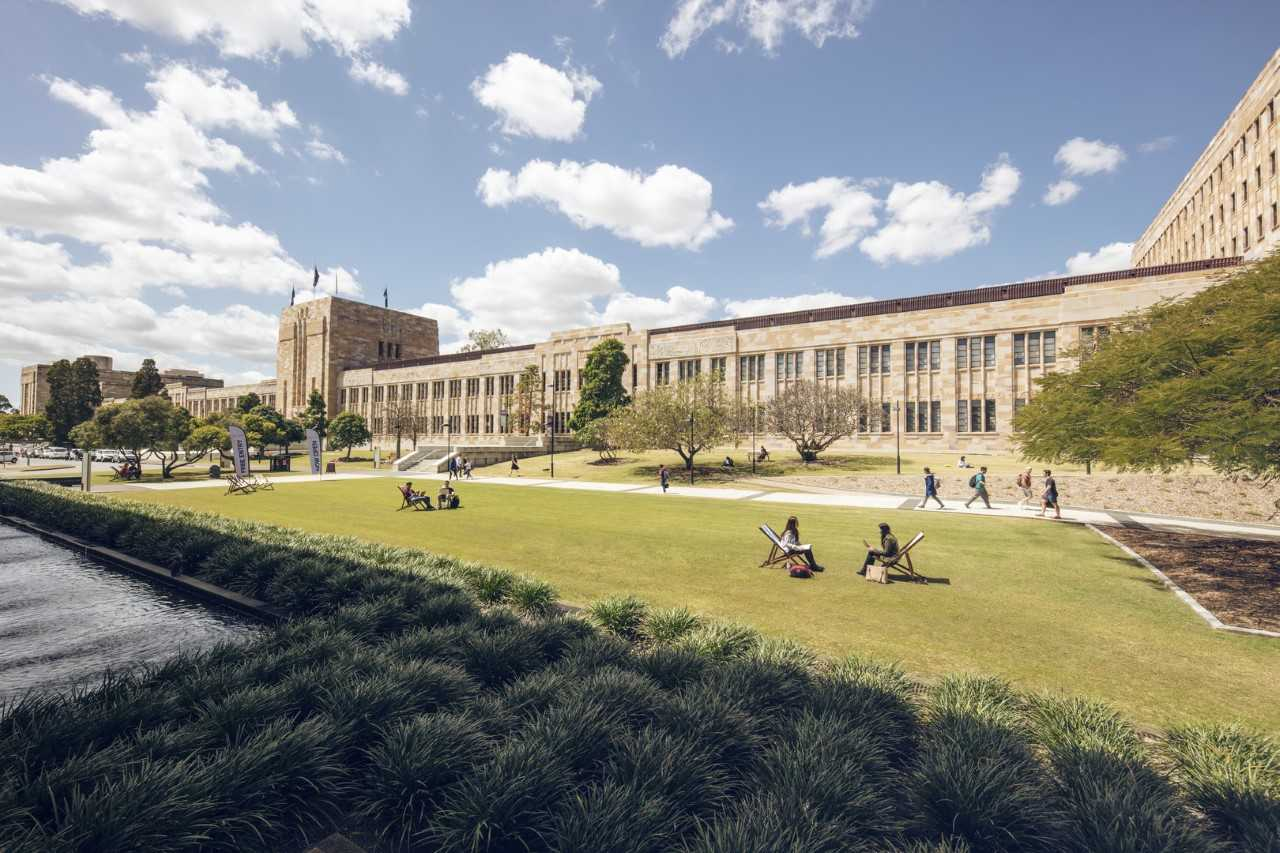
\includegraphics[width=1.0\textwidth]{Examples/FigureUQ}
\caption{The University Of Queensland}
\label{Fig:1}
\end{center}
\end{figure}

The Figure~\ref{Fig:1} represents beauty of the UQ campus.
% % ***************************************************
% Example of Flow Charts
% ***************************************************
%This example is provided for your reference only. DO NOT INCLUDE IN YOUR FINAL THESIS. 
\chapter{Example of Flow Charts}
\begin{figure}[h]
\caption{Flow Chart}
\label{Fig:FlowChart}
\begin{center}
\tikzstyle{decision} = [diamond, draw, fill=white!10, 
    text width=4.5em, text badly centered, node distance=3cm, inner sep=0pt]
\tikzstyle{block} = [rectangle, draw, fill=white!20, 
    text width=5em, text centered, rounded corners, minimum height=4em]
\tikzstyle{line} = [draw, -latex']
\tikzstyle{cloud} = [draw, ellipse,fill=white!20, node distance=3cm,
    minimum height=2em]
    
\begin{tikzpicture}[node distance = 2cm, auto]
    % Place nodes
    \node [block] (Step1) {initialize model};
    \node [cloud, left of=Step1] (expert) {expert};
    \node [cloud, right of=Step1] (system) {system};
    \node [block, below of=Step1] (identify) {identify candidate models};
    \node [block, below of=identify] (evaluate) {evaluate candidate models};
    \node [block, left of=evaluate, node distance=3cm] (update) {update model};
    \node [decision, below of=evaluate] (decide) {is best candidate better?};
    \node [block, below of=decide, node distance=3cm] (stop) {stop};
    % Draw edges
    \path [line] (Step1) -- (identify);
    \path [line] (identify) -- (evaluate);
    \path [line] (evaluate) -- (decide);
    \path [line] (decide) -| node [near start] {yes} (update);
    \path [line] (update) |- (identify);
    \path [line] (decide) -- node {no}(stop);
    \path [line,dashed] (expert) -- (Step1);
    \path [line,dashed] (system) -- (Step1);
    \path [line,dashed] (system) |- (evaluate);
\end{tikzpicture}
\end{center}
\end{figure}

Flow chart~\ref{Fig:FlowChart} is a simple example.
% % ***************************************************
% Example of Tables
% ***************************************************
%This example is provided for your reference only. DO NOT INCLUDE IN YOUR FINAL THESIS. 
\chapter{Example of Tables}

Here is a really simple table~\ref{Table}.


%\begin{table} : If you put no command after \begin{table} then this table will be printed anywhere in your pdf where LaTex finds the free space to put it. If you wish to specify where the table goes you have to give a command in LaTex after  \begin{table}. 
%
%There are different commands to put the table in different positions e.g. \begin{table}[h] LaTex will print the table in the same position that you put it in your source file, if there is enough space to print it
%N.B. it is important to note that commanding LaTeX to add a table in a specific place may result in formatting issues.

\begin{table}[h]
\caption{Name of the Australian Cities}
\begin{center}
\begin{tabular}{{|c|c|c|}}
\hline
\textbf{Number}& \textbf {Name}\\
\hline
      1& Brisbane\\
      2& Sydney\\
      3& Melbourne\\
      4& Canberra\\
      5& Perth\\
      6& Adelaide\\
      7& Hobart\\
      8& Darwin\\
\hline
\end{tabular}
\end{center}
\label{Table}
\end{table}


% ***************************************************
% Back Matter
%**************************************************** 
%COMMENT OUT IF YOU DO NOT WISH TO INCLUDE BACK MATTER.
% % ***************************************************
% Back Matter
% ***************************************************
% ADD AN ENDQUOTE HERE. If you do not wish to, delete this file.
\backmatter

\normalfont
\cleartooddpage

\pagestyle{empty}

\begin{table}[b!]
\begin{center}
% ********* Enter your quote within {} brackets: ********
\textit{Endquote goes here.}

% ********************************************************
\end{center}
\begin{flushright}
% ********* Enter your text below, as indicated: ********
Author of quote,\\
Source of quote

% ********************************************************
\end{flushright}
\end{table}

\end{document}
